\chapter[Word{}-formation]{Word-formation}\label{Para_3}

Papuan Malay has very little productive \isi{morphology}. Words are typically single root morphemes and word formation is limited to the two derivational processes of \isi{reduplication} and \isi{affixation}. Compounding is a third \isi{word-formation} process; it remains uncertain, however, to what degree it is a productive process. Inflectional \isi{morphology} is lacking, as nouns and verbs are not marked for any grammatical category such as gender, number, or case. There is also no voice system on verbs.



In discussing \isi{word-formation} in Papuan Malay, a major issue is to what degree these processes are productive. Following \citet[127]{Plag.2006}, the “productivity of a \isi{word-formation} process can be defined as its general potential to be used to create new words and as the degree to which this potential is exploited by the speakers”. Given this definition, the data in the corpus indicates that \isi{reduplication} in Papuan Malay is a very productive process, whereas \isi{affixation} has only very limited productivity. The productivity of \isi{compounding} as a \isi{word-formation} process remains debatable.



This chapter discusses two \isi{word-formation} processes in detail: \isi{affixation} in §\ref{Para_3.1} and \isi{compounding} in §\ref{Para_3.2}. Reduplication is described in \chapref{Para_4}. The main points of this chapter are summarized in §\ref{Para_3.3}.


\section{Affixation}\label{Para_3.1}
\subsection{Introduction}\label{Para_3.1.1}
In Papuan Malay, \isi{affixation} is a morphological process whereby an affix is attached to a \isi{lexical root} to derive new lexemes. This process typically applies to nouns and verbs.



The corpus contains a considerable number of morphologically complex lexical items with the 2,458-item \isi{word list} mentioned in §\ref{Para_1.11.6} including 523 affixed lexemes (21\%). The most commonly employed (historical) affixes are the prefixes \textscItal{ter-} ‘\textsc{acl}’, \textscItal{pe(n)-} ‘\textsc{ag}’, and \textscItal{ber-} ‘\textsc{vblz}’, the suffixes -\textitbf{ang} ‘\textsc{pat}’ and \textitbf{-nya} ‘\textsc{3possr}’, and the circumfix \textitbf{ke}-/-\textitbf{ang} ‘\textsc{nmlz}’.\footnote{The small caps designate the abstract representation of affixes that have more than one form of realization; prefixes \textscItal{ter-}, \textscItal{pe(n)-}, and \textscItal{ber-}, have two allomorphs each, namely \textitbf{ter}\textitbf{-} and \textitbf{ta}\textitbf{-} ( §\ref{Para_3.1.2.1}), \textitbf{pe(}\textscItal{n}\textitbf{)}- and \textitbf{pa(}\textscItal{n}\textitbf{)}- (small-caps \textscItal{n} represents the different realizations of the nasal) (§\ref{Para_3.1.4.1}), and \textitbf{ber}- and \textitbf{ba}- ( §\ref{Para_3.1.5.1}), respectively.}



Before examining these affixes in detail, the remainder of this introduction discusses methodological issues related to examining the productivity of \isi{affixation} in Papuan Malay.



Morphological patterns are considered to be productive if language users apply them “to create new well-formed complex words” by systematically extending the pattern “to new cases” \citep[67, 68]{Booij.2007}. By contrast, a morphological pattern is said to be unproductive when the morphological rule involved “is not used for coining new words” but “has become obsolete” (\citeyear*[68]{Booij.2007}). The productivity of a given pattern is a matter of degree, however, as pointed out by scholars such as \citet[49–58]{Aikhenvald.2007}, \citet[62–100]{Bauer.1983}, \citet[67–71]{Booij.2007}, or \citet[169–172]{Pike.1967}. This degree depends on the amount “to which the structural possibilities of a \isi{word-formation} pattern are actually used” \citep[68]{Booij.2007}. That is, depending on their functional load, some patterns are “fully active” or productive, while others are “inactive” or unproductive, with “semi-active” or semi-productive patterns found in-between \citep[169–171]{Pike.1967}.\footnote{\citet[169–171]{Pike.1967} talks about the “activeness of morphemes” rather than of “morphological patterns”.} Therefore, productivity is best viewed as a “cline” \citep[97]{Bauer.1983} or a “scalar phenomenon” (\citeyear*[126]{Bauer.2001}).\footnote{As {\citet[125]{Bauer.2001}} elaborates, however, there is an ongoing discussion among scholars “whether productivity is a gradable/scalar phenomenon or not”.} On such a cline of productivity, fully productive patterns are viewed as one endpoint, and completely unproductive patterns as the other endpoint of the continuum, with semi-productive patterns found in-between.



To investigate whether and to what degree Papuan Malay speakers employ a given affix to create new words, one technique would be to devise a test along the lines of \citegen{Aronoff.1978} “Productivity experiment”. This psycholinguistic experiment involved a lexical-decision task which required testees to make judgments about possible but non-occurring affixed words. That is, the testees had to judge whether or not these words were instances of English.



For the present study no productivity tests were conducted to determine whe\-ther and to what extent a given affix can be attached to Papuan Malay roots to derive new lexical items. Tests such as the mentioned lexical-decision tasks were considered unworkable due to the \isi{sociolinguistic profile} of the Papuan Malay speech variety and speech communities, discussed in §\ref{Para_1.5}:


\begin{itemize}
\item 
Functional distribution of Papuan Malay as the \textsc{low} variety, and Indonesian as the \textsc{high} variety, in terms of \citegen{Ferguson.1972} notion of diglossia;

\item 
Positive to somewhat am\isi{bivalent} language attitudes toward Papuan Malay; and

\item 
Lack of language awareness of many Papuan Malay speakers about the status of Papuan Malay as a language distinct from Indonesian.

\end{itemize}

Given this \isi{sociolinguistic profile} and the formal setting of a test situation as well as the fairly high degree of linguistic relatedness between Papuan Malay and Indonesian, an undesirable amount of interference from Indonesian was expected. This assumption is based on \citegen[1]{Weinreich.1953} definition of “interference” as “instances of deviation from the norms of either language which occur in the speech of bilinguals as a result of their familiarity with more than one language, i.e. as a result of language contact”. Even in a monolingual test situation, such interference would most likely have had a skewing impact on testees’ naïve judgments, given that, when in the “monolingual speech mode [\ldots] bilinguals rarely deactivate the other language totally”, as \citet[59]{Grosjean.1992} points out.



Given these problems, the attested affixes and derived words are instead examined in terms of six language internal and three language external factors. These factors were deemed relevant in examining the productivity of these affixes.


%\setcounter{itemize}{0}
\begin{enumerate}
\item 
Language internal factors


The affixes are examined with respect to the following six language internal factors: (a) syntactic properties, (b) type frequencies, token frequencies, and hapaxes, (c) form{}-function relationship between the derivation and its base word, (d) alternative strategies, (e) formally complex words with non-compositional semantics, and (f) status of the affixed lexemes as part of the Papuan Malay lexicon or as code-switches with Indonesian.


%\setcounter{itemize}{0}
\begin{enumerate}
\item 
Syntactic properties


If an affix is “polyfunctional”, that is, if it can take bases from more than one lexical category, this is taken as evidence that the process is more productive (\citealt[90--91]{Booij.2002}; see also \citealt{Zwanenburg.2000}). Hence, the syntactic properties for each affix are examined as to whether it can be attached to verbal, nominal, adverbial, and/or other bases. Likewise, the syntactic properties of the affixed lexemes are described, as to which word class they belong to.


\item 
Type frequencies, token frequencies and hapaxes\footnote{Type frequency is defined as “the number of types of a class of linguistic units in a corpus”, while token frequency refers to “the number of tokens of a linguistic unit or a class of linguistic units in a corpus” \citep[323]{Booij.2007}. Hapaxes are “new word types that occur only once in the corpus, and clearly do not belong to the set of established words” (\citeyear*[69]{Booij.2007}).}


If an affix is represented by a large number of words (high type frequency) which, in turn, have low token frequencies, this is taken as an indication that the \isi{affixation} process is more likely to be productive. (For the purposes of this study, type frequencies of ten or more are considered as “(relatively) high” while token frequencies of less than 20 are considered as “(relatively) low”.)



\citet[1044–1047]{Hay.2001} points out that “the frequency of the base form is involved in facilitating decomposability. When the base is more frequent than the whole, the word is easily and readily decomposable. However, when the derived form is more frequent than the base it contains, it is more difficult to decompose and appears to be less complex”. In terms of processing, morphologically complex words with a low relative frequency are accessed via their parts, that is, via a “decomposed access” or “parsing route”. Morphologically complex words with a high relative frequency, by contrast, are accessed as whole words via a “whole-word access” or “direct route” (\citeyear*[1055]{Hay.2001}).



Building on \citet{Hay.2001}, \citet[203–204]{Hay.2002} argue that “for an affix to remain productive, words containing that affix must be parsed sufficiently often that the resting activation level of that affix remains high”. The findings of their study confirm this link between productivity and parsing. \citet{Hay.2002} show that affixes which derive words with low relative frequencies and high rates of decomposition are more likely to be productive. By contrast, affixes which derive words with high relative frequencies and low rates of decomposition are less likely to be productive.



Along similar lines \citet[542]{Plag.2006b} discusses the decomposability of derived words with low token frequencies which “tend to be words that are unlikely to be familiar to the hearer”. They can, however, be understood if “an available \isi{word-formation} rule allows the decomposition of the newly encountered word into its constituent morphemes and thus the computation of the meaning on the basis of the meaning of the parts” (\citeyear*[542]{Plag.2006b}). Hence, productive morphological patterns tend to be characterized by “large numbers of low frequency words and small numbers of high frequency words, with the former keeping the rule alive. In contrast, unproductive morphological categories will be characterized by a preponderance of words with rather high frequencies and by a small number of words with low frequencies” (\citeyear*[542]{Plag.2006b}).



Among the derived words with low token frequency, hapaxes are especially useful in determining the productivity of a morphological pattern, as “the highest proportion of neologisms” is found here \citep[542]{Plag.2006b}; or in other words, “[the] higher the number of hapaxes, the greater the productivity” (\citeyear*[544]{Plag.2006b}). Therefore, as \citet[69–70]{Booij.2007} points out, “one might define the degree of productivity \textstyleChBold{P} of a particular morphological process as the proportion between the number of hapaxes of that type (n\textsubscript{1}) to the total number of tokens N” for that particular affix; a definition which is based on \citegen[115]{Baayen.1992} formula P~=~n\textsubscript{1}/N.



For the present study, however, it remains unclear to what extent the attested hapaxes are useful in determining productivity. That is, the limited size of the corpus makes it difficult to verify which hapaxes are neologisms in Papuan Malay and which ones merely reflect the limited size of the corpus. Moreover, the literature does not mention thresholds which would allow interpreting a calculated P value in terms of the degree of productivity of a given morphological pattern. For the interested reader, however, the number of hapaxes and their respective P values for each affix are given in footnotes throughout this chapter.



\item 
Form-function relationship between the derivation and its base\label{List_3.1.c}


Typical derivational processes include nominalization, verbalization, or class-preserving valency-changing operations, among others. In each case, the derivational process “results in the creation of a new word with a new meaning”, as {\citet[35]{Aikhenvald.2007}} points out.



Following \citet[240, 323]{Booij.2007}, one “necessary” albeit not “sufficient” \isi{condition} for the productivity of such derivational processes is their transparency, which is defined as “the presence of a systematic form-meaning correspondence in a morphologically complex form”. Therefore, if the form-function relationship between the affixed lexemes and their base is transparent, this is taken as evidence that a given \isi{affixation} process is more productive. If, by contrast, this relationship is opaque, this is considered evidence that the process is less productive.



For the present study, pairs of words in which the affixed words and their respective bases have the same semantics are not taken as parts of a larger derivational paradigm. Instead these sets are taken as pairs of words belonging to different speech varieties, namely Papuan Malay and Indonesian. This conclusion is based on the fact that, in general, nonstandard varieties of Malay “have lost most or all of this system of \isi{affixation}”, whereas “Standard Malay exhibits a rich system of \isi{affixation}” \citep[20]{Paauw.2009}. Hence, for pairs of words with the same semantics, the unaffixed base words are taken to be the native Papuan Malay lexemes, whereas the affixed words are taken to be code-switches with the corresponding Indonesian lexemes.


\item 
Alternative strategies


If speakers employ alternative strategies that do not involve \isi{affixation} and that express the same meanings as the affixed forms, these alternative strategies are taken as evidence that the \isi{affixation} process is less productive.



\item 
Formally complex words with non-compositional semantics


Affixed lexemes for which there is no corresponding base have lost their status as complex words. They are so-called “formally complex words” \citep[17]{Booij.2007}. Such a word “behaves as a complex word although there is no corresponding semantic complexity” (\citeyear*[13]{Booij.2007}). A high number of formally complex words are taken as evidence that the \isi{affixation} process is less productive. Their non-compositional semantics suggest that these lexemes are either lexicalized forms or code-switches with Indonesian. (For each affix, the number of formally complex words is given with a few examples. Given, however, that they have lost their status as complex words, these items are not further discussed.)



\item 
Status of the affixed lexemes as part of the Papuan Malay lexicon or as code-switches with Indonesian\label{List_3.1.f}


If a large number of affixed lexemes are not part of the Papuan Malay lexicon but code-switches with Indonesian, this is taken as evidence that the derivation process for a given affix is less productive.



Sources such as \citet{Jones.2007}, or \citet{Tadmor.2009} allow the identification of foreign, non-Malay loanwords in the corpus. They do not, however, allow identifying code-switches with Indonesian. Hence, an alternative approach was deemed necessary to explore whether the affixed lexemes are part of the Papuan Malay lexicon or constitute code-switches with Indonesian.



All 533 attested affixed lexemes were discussed with a Papuan Malay consultant who has a high level of language awareness, both with respect to Papuan Malay and to Indonesian. Based on his knowledge of both languages, the consultant classified the affixed lexemes as “Papuan Malay” or “borrowings from Indonesian”. The statement that a lexeme is considered to be Papuan Malay does not imply, however, that the respective lexeme does not exist in other Malay varieties as well. Across Southeast Asia, all Malay varieties have large sets of shared lexical items; this also applies to Papuan Malay, the other \ili{eastern Malay varieties} and also to Indonesian.



While the consultant’s tentative classification is subjective and not necessarily representative, it provides one more piece of evidence as to the potential productivity of the attested affixes. In \tabref{Table_3.1} to \tabref{Table_3.24}, these alleged borrowings or code-switches with (Standard) Indonesian are underlined.


\end{enumerate}
\item 
{Language external factors\label{List_3.2}}: Variables of the \isi{communicative event}


The affixes were examined as to whether they are employed without sociolinguistic restrictions or whether their use is conditioned by variables of the speech situation in terms of \citegen[86]{Fishman.1965} “domains of language choice”. The main factors which influence language choices are (1) the topics discussed, (2) the relationships between the interlocutors, and (3) the locations where the communication takes place (\citeyear*[67, 75]{Fishman.1965}). Speaker education levels are a fourth pertinent factor.



If the use of the affixes seems to be conditioned by language external factors, this is taken as evidence that the \isi{affixation} process is less productive. For the present study, the pertinent “domains of language choice” are (a) the topics, (b) speaker education levels, and (c) the relationships between the interlocutors, all of which are discussed in the following. The locations of communication were not considered pertinent domains since all recorded conversations took place in the same informal setting of the home. (For details on the \isi{sociolinguistic profile} of Papuan Malay, see §\ref{Para_1.5}.)


%\setcounter{itemize}{0}
\begin{enumerate}
\item 
Speaker education levels\label{List_3.2.a}


In West Papua, as is typical of diglossic situations, the \textsc{high} variety Indonesian is acquired in school. Given their amount of access to the \textsc{high} variety, better-educated speakers are more likely to display language behaviors influenced by the \textsc{high} variety Indonesian than less-educated speakers. Therefore, if better-educated speakers employ a particular affix considerably more often than less-educated ones, this is taken as evidence that the affixed lexemes are not the result of a productive process but that they constitute code-switches with Indonesian. (See also Factor 1 ``Speaker education levels'' in §\ref{Para_1.5.1}.)



\item 
Topics\label{List_3.2.b}


Following {\citet[71]{Fishman.1965}}, the topics under discussion may also bring “another language to the fore” as “certain topics are somehow handled better in one language than in another”. This notion of topical regulation suggests that Papuan Malay speakers consider Indonesian, and not Papuan Malay, the appropriate language to use when discussing \textsc{high} topics associated with formal domains such as politics, education, or religion. Therefore, if Papuan Malay speakers use a particular affix much more often when discussing \textsc{high} topics than when discussing casual daily-life issues (\textsc{low} topics), this is taken as evidence that the affixed lexemes are code-switches with Indonesian. This applies especially to less-educated Papuans, as better-educated Papuans already display a general tendency to include Indonesian features when speaking Papuan Malay, although this tendency is more pronounced when the latter discuss \textsc{high} topics. (See also Factor 2 ``Topical regulation'' in §\ref{Para_1.5.1}.)


\item 
Relationships between interlocutors\label{List_3.2.c}

Given the diglossic distribution of Papuan Malay and Indonesian, it is expected that the language behavior of Papuans shows influences from the \textsc{high} variety Indonesian when they interact with fellow-Papuans of higher status or with group outsiders. As discussed under Factor 3 ``Relationships between interlocutors'' in §\ref{Para_1.5.1}, the use of features from the \textsc{high} variety serves to signal social inequality, distance, and formality. Therefore, if speakers use a given affix much more often when conversing with interlocutors of higher status or with group outsiders than when interacting with peers, this is taken as evidence that the affixed lexemes are code-switches with Indonesian. Again, this applies especially to less-educated Papuans, given that better-educated Papuans already show a general tendency to “dress-up” their Papuan Malay with Indonesian features, although this tendency is more marked when the latter interact with group outsiders, such as the author. (See also Factor 3 ``Relationships between interlocutors'' in §\ref{Para_1.5.1}.)

\end{enumerate}
\end{enumerate}

In examining the attested affixes and affixed lexemes as outlined above, none of the factors was taken in isolation. Instead, the findings pertaining to all nine factors were taken together as an indication of the degree of productivity for the affix in question. The results of this multifaceted investigation indicate that in Papuan Malay:



\begin{itemize}
\item 
Prefix \textscItal{ter-} ‘\textsc{acl}’ and suffix -\textitbf{ang} ‘\textsc{pat}’ are somewhat productive;

\item 
Prefix \textscItal{pe(n)-} ‘\textsc{ag}’ is, at best, marginally productive; and

\item
Prefix \textscItal{ber-} ‘\textsc{vblz}’, suffix \textitbf{-nya} ‘\textsc{3possr}’, and circumfix \textitbf{ke}-/-\textitbf{ang} ‘\textsc{nmlz}’ are unproductive.

\end{itemize}

The unproductive derivations are considered to be lexicalized forms borrowed into the language or code-switches with Indonesian; in the examples, however, no attempt is made to distinguish the two.



In the following, the six affixes are discussed in detail in terms of the factors outlined above: \textscItal{ter-} in §\ref{Para_3.1.2}, -\textitbf{ang} in §\ref{Para_3.1.3}, \textscItal{pe(n)-} in §\ref{Para_3.1.4}, \textscItal{ber-} in §\ref{Para_3.1.5}, \mbox{\textitbf{-nya}} in §\ref{Para_3.1.6}, and \textitbf{ke}-/-\textitbf{ang} in §\ref{Para_3.1.7}. For the three somewhat productive affixes (\textscItal{ter-}, -\textitbf{ang}, and \textscItal{pe(n)-}) the mentioned variables of the \isi{communicative event} are investigated in detail within the respective sections. For the remaining three affixes (\textscItal{ber-}, \textitbf{-nya}, and \textitbf{ke}-/-\textitbf{ang}) the variables of the \isi{communicative event} are summarily discussed in §\ref{Para_3.1.8}. The main points on \isi{affixation} are summarized in §\ref{Para_3.3}.


\subsection[Prefix {\TER}- ‘\textsc{acl}’]{Prefix \textscItal{ter-} ‘\textsc{acl}’}\label{Para_3.1.2}
Affixation with \textscItal{ter-} ‘\textsc{acl}’ derives \isi{monovalent} verbs from verbal bases. The derived verbs denote accidental or unintentional actions or events, as shown in (\ref{Example_3.1}). This derivation process appears to be somewhat productive in Papuan Malay, as discussed below.

\ea
\label{Example_3.1}
\gll {bos} {pagi} {{su}} {{br\bluebold{–}angkat}} {{ke}} {{Sarmi}} {{begini}} {adu}\\ %
 boss  morning  {already}  {\textsc{vblz}\bluebold{–}leave}  {to}  {Sarmi}  {like.this}  oh.no!\\
\gll {sial–ang}  {\bluebold{ter–paksa}}  {tong}  {dua}  {jalang}  {kaki}\\
 {be.unfortunate–\textsc{pat}}  {\textsc{acl}–force}  {\textsc{1pl}}  {two}  {walk}  {foot}\\
\glt 
‘as the boss had already left for \ili{Sarmi} in the morning, oh no, damn it!, the two of us \bluebold{were} \bluebold{forced} to walk on foot’ \textstyleExampleSource{[080921-002-Cv.0001]}\\
\z


Prefix \textscItal{ter-} is a reflex of Proto-\ili{Malayic} *\textitbf{t}\textscItal{a}\textitbf{r}-, which, following \citet[155]{Adelaar.1992}, “contributed the notion of unintentionality or feasibility to the VTR or VDI to which it was affixed”. In Standard Malay, “\textitbf{tər}- denotes an ‘accidental’ state, process or action” when affixed to \isi{bivalent} bases and “a superlative degree” when affixed to \isi{monovalent} bases (\citeyear*[150–151]{Adelaar.1992}). In \ili{eastern Malay varieties}, the prefix also denotes accidental or unintentional actions, or events that happened unexpectedly or unintentionally. These productive uses of the prefix are attested for \ili{Ambon Malay} \citep[98]{vanMinde.1997}, \ili{Banda Malay} {\citep[250]{Paauw.2009}}, \ili{Kupang Malay} {\citep[46]{Steinhauer.1983}}, \ili{Larantuka Malay} {\citep[256]{Paauw.2009}}, \ili{Manado Malay} \citep[22]{Stoel.2005}, and North Moluccan / \ili{Ternate Malay} (\citealt[18]{Taylor.1983};\footnote{While \citet[18]{Taylor.1983} considers the prefix to be productive, \citet[4]{Voorhoeve.1983} believes that it is unproductive.} \citealt[133]{Litamahuputty.2012}).



The corpus includes 43 \isi{monovalent} verbs (167 tokens) prefixed with \textscItal{ter-}:\footnote{The 43 verbs include 21 hapaxes (P=0.1257); the 38 \isi{bivalent} verbs include 17 hapaxes (P=0.1111); the five \isi{monovalent} verbs include four hapaxes (P=0.2857).}


%\setcounter{itemize}{0}

\begin{enumerate}
\item 
Verbs with \isi{bivalent} bases (38 items with 153 tokens)

\item 
Verbs with \isi{monovalent} bases (five items with 14 tokens)

\end{enumerate}

The corpus also contains ten formally complex words with non-compositional semantics, such as \textitbf{tertawa} ‘laugh’, \textitbf{tergrak} ‘be moved’, or \textitbf{trapung} ‘be drifting’.\footnote{The historical roots \textitbf{tawa}, \textitbf{grak}, or \textitbf{apung} do not exist in Papuan Malay.}



Before discussing \textscItal{ter-}\isi{affixation} of \isi{bivalent} bases in §\ref{Para_3.1.2.2} and of \isi{monovalent} bases in §\ref{Para_3.1.2.3}, the \isi{allomorphy} of \textscItal{ter-} is examined in §\ref{Para_3.1.2.1}. Variables of the \isi{communicative event} that may impact the use of \textscItal{ter-} are explored in §\ref{Para_3.1.2.4}. The main points on prefix \textscItal{ter-} are summarized and evaluated in §\ref{Para_3.1.2.5}.


\subsubsection[Allomorphy of ter-]{Allomorphy of \textscItalBold{ter-}}\label{Para_3.1.2.1}

Prefix \textscItal{ter-} has two allomorphs, \textitbf{ter}\textitbf{-} and \textitbf{ta}\textitbf{-}. The allomorphs are not governed by phonological processes.



The form \textitbf{ter}\textitbf{-}, in turn, has three allomorphs that are the effect of, what \citet[75]{Booij.2007} calls “morphologically conditioned phonological rules”. More specifically, the three allomorphs are conditioned by the word-initial segment of the base word, as shown in \tabref{Table_3.1}: /\textstyleChCharisSIL{tɛr-}/, /\textstyleChCharisSIL{tɛ-}/, and /\textstyleChCharisSIL{tr-}/. Most commonly, \textitbf{ter}- is realized as /\textstyleChCharisSIL{tɛr-}/. With onset rhotic /\textstyleChCharisSIL{r}/, however, it is realized as /\textstyleChCharisSIL{tɛ-}/. With onset vowels, the prefix is usually realized as /\textstyleChCharisSIL{tr-}/.


\begin{table}
\caption{ Realizations of allomorph \textitbf{ter}-}\label{Table_3.1}

\begin{tabular}{lll}
\lsptoprule
 \multicolumn{1}{c}{\textitbf{ter}-base} & \multicolumn{1}{c}{Orthogr.} &  \multicolumn{1}{c}{Gloss}\\
\midrule



/\textstyleChCharisSIL{tɛr}–\textstyleChCharisSIL{pukul}/ & \textitbf{terpukul} & ‘be beaten’\\

/\textstyleChCharisSIL{tɛ}–\textstyleChCharisSIL{rɛndam}/ & \textitbf{terendam} & ‘be soaked’\\

/\textstyleChCharisSIL{tr}–a\textstyleChCharisSIL{ŋkat}/ & \textitbf{trangkat} & ‘be lifted’\\

\lspbottomrule
\end{tabular}
\end{table}

Allomorph \textitbf{ta}- is used in about one third of the affixed items; that is, 17 items with a total of 41 \textitbf{ta}- tokens, listed in \tabref{Table_3.2}. Some of the derived items are alternatively realized with allomorph \textitbf{ter}-. Hence, for each item the frequencies for \textitbf{ta}- and for \textitbf{ter}- are given.\footnote{In addition, the 2,459-item \isi{word list} (see \chapref{Para_2}, p. \pageref{Para_2}) contains five items realized with /\textstyleChCharisSILviiivpt{ta-}/ rather than with /\textstyleChCharisSILviiivpt{tɛr-}/: /\textstyleChCharisSILviiivpt{tabla}/ ‘be cracked open’, /\textstyleChCharisSILviiivpt{takumpul}/ ‘be gathered’, /\textstyleChCharisSILviiivpt{takupas}/ ‘be peeled’, /\textstyleChCharisSILviiivpt{tamasuk}/ ‘be included’, and /\textstyleChCharisSILviiivpt{tatutup}/ ‘be closed’. In the corpus these items are realized with /\textstyleChCharisSILviiivpt{tɛr-}/. Further, the \isi{word list} also includes three items realized with /\textstyleChCharisSILviiivpt{tɛr-}/ whereas in the corpus these items are most commonly realized with /\textstyleChCharisSILviiivpt{ta-}/: \textitbf{talempar} ‘be thrown’, \textitbf{talipat} ‘be folded’, and \textitbf{tarangkat} ‘be lifted up’.} If in a greater number of tokens the prefix is realized with /\textstyleChCharisSIL{ta-}/ than with /\textstyleChCharisSIL{tɛr-}/, then its orthographic representation is \textitbf{ta}- as in \textitbf{tagoyang} ‘be shaken’. If both realizations occur with the same frequency, then the orthographic representation follows its realization in the recorded texts, as in \textitbf{terlepas} ‘be loose’.


\begin{table}
\caption{Realizations of allomorph \textitbf{ta}-}\label{Table_3.2}


\begin{tabular}{lllrr}
\lsptoprule

 \multicolumn{1}{c}{\textitbf{ta}-base} & \multicolumn{1}{c}{Orthogr.} & \multicolumn{1}{c}{Gloss} & \multicolumn{1}{c}{\textitbf{ta}- \#} &  \multicolumn{1}{c}{\textitbf{ter}- \#}\\
\midrule
/\textstyleChCharisSIL{ta}–\textstyleChCharisSIL{g}ɔ\textstyleChCharisSIL{jaŋ}/ & \textitbf{tagoyang} & ‘be shaken’ &  9 &  0\\

/\textstyleChCharisSIL{ta}–\textstyleChCharisSIL{putar}/ & \textitbf{taputar} & ‘be turned around’ &  7 &  2\\

/\textstyleChCharisSIL{ta}–\textstyleChCharisSIL{lipat}/ & \textitbf{talipat} & ‘be folded’ &  6 &  1\\

/\textstyleChCharisSIL{ta}–\textstyleChCharisSIL{lɛmpar}/ & \textitbf{talempar} & ‘be thrown’ &  4 &  1\\

/\textstyleChCharisSIL{ta}–\textstyleChCharisSIL{guliŋ}/ & \textitbf{taguling} & ‘be rolled over’ &  3 &  0\\

/\textstyleChCharisSIL{ta}–\textstyleChCharisSIL{gant}ɔ\textstyleChCharisSIL{ŋ}/ & \textitbf{tergantong} & ‘be dependent’ &  1 &  6\\

/\textstyleChCharisSIL{ta}–\textstyleChCharisSIL{lɛpas}/ & \textitbf{terlepas} & ‘be loose’ &  1 &  1\\

/\textstyleChCharisSIL{ta}–\textstyleChCharisSIL{balik}/ & \textitbf{tabalik} & ‘be turned upside down’ &  1 &  0\\

/\textstyleChCharisSIL{ta}–\textstyleChCharisSIL{bantiŋ}/ & \textitbf{tabanting} & ‘be tossed around’ &  1 &  0\\

/\textstyleChCharisSIL{ta}–\textstyleChCharisSIL{tʃukur}/ & \textitbf{tacukur} & ‘be scalped’ &  1 &  0\\

/\textstyleChCharisSIL{ta}–\textstyleChCharisSIL{gait}/ & \textitbf{tagait} & ‘be hooked &  1 &  0\\

/\textstyleChCharisSIL{ta}–\textstyleChCharisSIL{hambur}/ & \textitbf{tahambur} & ‘be scattered about’ &  1 &  0\\

/\textstyleChCharisSIL{ta}–\textstyleChCharisSIL{kantʃiŋ}/ & \textitbf{takancing} & ‘be locked’ &  1 &  0\\

/\textstyleChCharisSIL{ta}–\textstyleChCharisSIL{lɛm}/ & \textitbf{talem} & ‘be glued’ &  1 &  0\\

/\textstyleChCharisSIL{ta}–\textstyleChCharisSIL{sala}/ & \textitbf{tasala} & ‘be mistaken’ &  1 &  0\\

/\textstyleChCharisSIL{ta}–\textstyleChCharisSIL{tikam}/ & \textitbf{tatikam} & ‘be stabbed’ &  1 &  0\\

/\textstyleChCharisSIL{ta}–\textstyleChCharisSIL{t}ɔ\textstyleChCharisSIL{ŋkat}/ & \textitbf{tatongkat} & ‘be beaten’ &  1 &  0\\

\lspbottomrule
\end{tabular}
\end{table}

In realizing the prefix most commonly as \textitbf{ter}- rather than as \textitbf{ta}-, Papuan Malay differs from other \ili{eastern Malay varieties} such as \ili{Ambon Malay} \citep[98]{vanMinde.1997}, \ili{Banda Malay} \citep[250]{Paauw.2009}, \ili{Kupang Malay} \citep[46]{Steinhauer.1983}, \ili{Manado Malay} \citep[22]{Stoel.2005}, and North Moluccan / \ili{Ternate Malay} (\citealt[18]{Taylor.1983}; \citealt[4]{Voorhoeve.1983}; \citealt[133]{Litamahuputty.2012}). In these varieties the prefix is always realized as \textitbf{ta}-. Instead, the \textscItal{ter-}prefixed items have more resemblance with the corresponding items in Indonesian, where the prefix is realized as \textitbf{ter}-. In addition, in \ili{Larantuka Malay} the prefix is also realized as \textitbf{tə(r)}- {\citep[253]{Paauw.2009}}. The different behavior of Papuan Malay \textscItal{ter-} supports the conclusion put forward in §\ref{Para_1.8} that the history of Papuan Malay is different from that of the other \ili{eastern Malay varieties}.


\subsubsection[Prefixed items derived from {bivalent} verbal bases]{Prefixed items derived from {bivalent} verbal bases}\label{Para_3.1.2.2}

The corpus contains 38 \textscItal{ter-}prefixed lexemes (with 153 tokens) with \isi{bivalent} \isi{verbal base} words (BW), as listed in \tabref{Table_3.3} and \tabref{Table_3.3a}. The \isi{affixation} derives \isi{monovalent} verbs with non-agent arguments through a valency-changing operation, in which \textscItal{ter-} removes agent arguments. All but one of the derived lexemes are low frequency words (37 lexemes, attested with less than 20 tokens). Besides, the token frequencies for the respective bases are (much) higher for most of the derived words (29 lexemes).

\begin{table} 
\caption[Affixation with {ter-} of \isi{bivalent} verbal bases]{Affixation with \textscItal{ter-} of \isi{bivalent} verbal bases\footnote{As mentioned in language internal factor (\ref{List_3.1.f}) in §\ref{Para_3.1.1} (p. \pageref{List_3.1.f}),
  alleged borrowings or code-switches with (Standard) Indonesian are underlined.}}
\label{Table_3.3}
\centering
%\setlength{\tabcolsep}{1.1mm}
\begin{tabularx}{\textwidth}{llllrr}
\lsptoprule
 \multicolumn{1}{c}{BW} & \multicolumn{1}{c}{Gloss} & \multicolumn{1}{c}{Item} & \multicolumn{1}{c}{Gloss} & \multicolumn{1}{c}{\textscItal{ter-} \#} & \multicolumn{1}{c}{BW \#}\\
\midrule
\textitbf{jadi} & ‘become’ & \textitbf{terjadi} & ‘happen’ &  39 &  120\\

\textitbf{paksa} & ‘force’ & \textitbf{terpaksa} & ‘be forced’ &  10 &  10\\

\textitbf{masuk} & ‘enter’ & \textitbf{termasuk} & ‘be included’ &  9 &  261\\

\textitbf{putar} & ‘turn around’ & \textitbf{taputar} & ‘be turned around’ &  9 &  33\\

\textitbf{goyang} & ‘shake’ & \textitbf{tagoyang} & ‘be shaken’ &  9 &  10\\

\textitbf{gantong} & ‘suspend’ & \textitbf{tergantong} & ‘be dependent’ &  7 &  14\\

\textitbf{lipat} & ‘fold’ & \textitbf{talipat} & ‘be folded’ &  7 &  1\\

\textitbf{buka} & ‘open’ & \textitbf{terbuka} & ‘be opened’ &  6 &  1\\

\textitbf{angkat} & ‘lift’ & \textitbf{trangkat} & ‘be lifted’ &  5 &  81\\

\textitbf{lempar} & ‘throw’ & \textitbf{talempar} & ‘be thrown’ &  5 &  12\\

\textitbf{rendam} & ‘soak’ & \textitbf{terendam} & ‘be soaked’ &  5 &  1\\

\textitbf{pukul} & ‘beat’ & \textitbf{terpukul} & ‘be beaten’ &  4 &  59\\

\textitbf{bakar} & ‘burn’ & \textitbf{terbakar} & ‘be burnt’ &  3 &  55\\

\textitbf{guling} & ‘roll over’ & \textitbf{taguling} & ‘be rolled over’ &  3 &  2\\

\textitbf{tutup} & ‘close’ & \textitbf{tertutup} & ‘be closed’ &  3 &  53\\

\textitbf{bagi} & ‘divide’ & \textitbf{terbagi} & ‘be split up’ &  2 &  66\\

\textitbf{tarik} & ‘pull’ & \textitbf{tertarik} & ‘be pulled’ &  2 &  32\\

\textitbf{lepas} & ‘free’ & \textitbf{talepas} & ‘be loose’ &  2 &  23\\

\textitbf{kumpul} & ‘gather’ & \textitbf{terkumpul} & ‘be collected’ &  2 &  16\\

\textitbf{tolak} & ‘push away’ & \textitbf{tertolak} & ‘be rejected’ &  2 &  11\\

\textitbf{kupas} & ‘peel’ & \textitbf{terkupas} & ‘be peeled’ &  2 &  1\\

\textitbf{buat} & ‘make’ & \textitbfUndl{terbuat} & ‘be made’ &  1 &  135\\

\textitbf{kenal} & ‘know’ & \textitbf{terkenal} & ‘be well-known’ &  1 &  57\\

\textitbf{balik} & ‘turn over’ & \textitbf{tabalik} & ‘be turned over’ &  1 &  37\\

\textitbf{ganggu} & ‘disturb’ & \textitbf{terganggu} & ‘be disturbed’ &  1 &  18\\

\textitbf{bla} & ‘split’ & \textitbf{terbla} & ‘be split’ &  1 &  13\\

\textitbf{pengaru} & ‘influence’ & \textitbfUndl{terpengaru} & ‘be affected’ &  1 &  7\\

\textitbf{banting} & ‘throw’ & \textitbf{tabanting} & ‘be tossed around’ &  1 &  6\\
\lspbottomrule
\end{tabularx} 
\end{table}

\begin{table}
\begin{minipage}{\textwidth}
\caption[Affixation with {ter-} of \isi{bivalent} verbal bases continued]{Affixation with \textscItal{ter-} of \isi{bivalent} verbal bases continued\footnote{As mentioned in language internal factor (\ref{List_3.1.f}) in §\ref{Para_3.1.1} (p. \pageref{List_3.1.f}),
  alleged borrowings or code-switches with (Standard) Indonesian are underlined.}}
\label{Table_3.3a}
\centering
\begin{tabularx}{\textwidth}{llllrr}
\lsptoprule
 \multicolumn{1}{c}{BW} & \multicolumn{1}{c}{Gloss} & \multicolumn{1}{c}{Item} & \multicolumn{1}{c}{Gloss} & \multicolumn{1}{c}{\textscItal{ter-} \#} & \multicolumn{1}{c}{BW \#}\\
 \midrule
\textitbf{tukar} & ‘exchange’ & \textitbf{tertukar} & ‘get changed’ &  1 &  6\\

\textitbf{tongkat} & ‘cane’ & \textitbf{tatongkat} & ‘be beaten up’ &  1 &  5\\

\textitbf{singgung} & ‘offend’ & \textitbf{tersinggung} & ‘be offended’ &  1 &  3\\

\textitbf{cinta} & ‘love’ & \textitbfUndl{tercinta} & ‘be beloved’ &  1 &  3\\

\textitbf{cukur} & ‘flatten’ & \textitbf{tacukur} & ‘be scalped’ &  1 &  2\\

\textitbf{hambur} & ‘scatter’ & \textitbf{tahambur} & ‘be scattered about’ &  1 &  1\\

\textitbf{wesel} & ‘transfer’ & \textitbfUndl{terwesel} & ‘be transferred’ &  1 &  2\\

\textitbf{tikam} & ‘stab’ & \textitbf{tatikam} & ‘be stabbed’ &  1 &  2\\

\textitbf{kancing} & ‘lock’ & \textitbf{takancing} & ‘be locked’ &  1 &  0\\

\textitbf{lem} & ‘glue’ & \textitbfUndl{talem} & ‘be glued’ &  1 &  0\\

\lspbottomrule
\end{tabularx}
\end{minipage}
\end{table}
The derived verbs denote accidental or unintentional states, processes, or actions. The term “accidental” covers “such concepts as involuntary, unmotivated, agentless, sudden, and unexpected action (or state resulting therefrom)”, employing \citegen[150]{Adelaar.1992} terminology. Hence, \textscItal{ter-} is glossed as ‘\textsc{acl}’ (‘accidental’). Two \textscItal{ter-}prefixed items are given in context: \textitbf{tagoyang} ‘be shaken’ in (\ref{Example_3.2}) and \textitbf{tertutup} ‘be closed’ in (\ref{Example_3.4}). Both examples, together with the one in (\ref{Example_3.3}), illustrate how \textscItal{ter-} decreases \isi{valency} by “removing agent-like participants”.


\newpage
\begin{styleExampleTitle}
{Prefix \textscItal{ter-}: Semantics of \isi{bivalent} verbal bases and derived lexemes}
\end{styleExampleTitle}

\ea
\label{Example_3.2}
\gll {de} {bilang,} {mama} {sa} {liat} {pohong} {ini} {de} {\bluebold{ta–goyang}}\\ %
 \textsc{3sg}  say  mother  \textsc{1sg}  see  tree  \textsc{d.prox}  \textsc{3sg}  \textsc{acl}–shake\\
\glt 
‘she said, ``mama, I saw this tree, it was \bluebold{shaking}''' \textstyleExampleSource{[080917-008-NP.0031]}
\z
\ea
\label{Example_3.3}
\gll {\ldots} {bapa} {Markus} {S.} {doseng} {satu} {de} {\bluebold{goyang}} {kepala}\\ %
{}   father  Markus  S.  lecturer  one  \textsc{3sg}  shake  head\\
\glt 
‘{\ldots} Mr. Markus S., a certain lecturer, he \bluebold{shook} (his) head’ \textstyleExampleSource{[080917-010-CvEx.0194]}
\z
\ea
\label{Example_3.4}
\gll {kalo} {ko} {\bluebold{tutup}} {pintu} {berkat} {juga} {\bluebold{ter–tutup}} {\ldots}\\ %
 if  \textsc{2sg}  close  door  blessing  also  \textsc{acl}–close  \\
\glt 
‘if you \bluebold{close} the door (of your house), the blessing is also \bluebold{closed off} [(because) guests cannot come into (your) house]’ \textstyleExampleSource{[081110-008-CvNP.0096]}
\z


Of the 38 \textscItal{ter-}prefixed \isi{bivalent} verbs, one Papuan Malay consultant classified four as borrowings from \ili{Standard Indonesian} (SI-borrowings) (see language internal factor (\ref{List_3.1.f}) in §\ref{Para_3.1.1}, p. \pageref{List_3.1.f}), namely \textitbf{terbuat} ‘be made’, \textitbf{terpengaru} ‘be influenced’, \textitbf{tercinta} ‘be beloved’, and \textitbf{terwesel} ‘be transferred’ (in \tabref{Table_3.3} these items are underlined). The same consultant also stated that Papuan Malay speakers usually employ the respective bases rather than the prefixed forms. One such contrastive set of examples is given in (\ref{Example_3.5}) and (\ref{Example_3.6}). Instead of using the prefixed form \textitbf{terpengaru} ‘be influenced’, as in (\ref{Example_3.5}), speakers more often employ the base \textitbf{pengaru} ‘influence’ in the sense of ‘be influenced’, as in (\ref{Example_3.6}).


\newpage
\begin{styleExampleTitle}
{Prefix \textscItal{ter-}: Use patterns of base words versus derived lexemes}
\end{styleExampleTitle}
\ea
\label{Example_3.5}
\gll {\ldots} {tapi} {de} {ana} {juga} {cepat} {ikut} {\bluebold{ter–pengaru}}\\ %
 { }    but  \textsc{3sg}  child  also  be.fast  follow  \textsc{acl}–influence\\
\glt 
‘{\ldots} but he/she, a kid, also quickly follows (others) to \bluebold{be influenced}’ \textstyleExampleSource{[080917-010-CvEx.0001]}
\z
\ea
\label{Example_3.6}
\gll {de} {su} {\bluebold{pengaru}} {dengang} {orang{\Tilde}orang} {yang} {minum}\\ %
 \textsc{3sg}  already  influence  with  \textsc{rdp}{\Tilde}person  \textsc{rel}  drink\\
\glt
‘he has already \bluebold{been influenced} by people who drink’ \textstyleExampleSource{[080919-007-CvNP.0018]}
\z


\subsubsection[Prefixed items derived from {monovalent} verbal bases]{Prefixed items derived from {monovalent} verbal bases}\label{Para_3.1.2.3}
The corpus contains five \textscItal{ter-}prefixed lexemes (with 14 tokens) with \isi{monovalent} verbal bases, as listed in \tabref{Table_3.4}. Contrasting with the \isi{affixation} of \isi{bivalent} bases, \textscItal{ter-}{affixa\-tion} of \isi{monovalent} bases is not a valency-changing operation, nor does it derive verbs with non-agent arguments. Instead, \textscItal{ter-} downplays the level of control of its arguments by deriving \isi{monovalent} verbs which denote accidental or unintentional states or actions, such as \textitbf{terlambat} ‘be late’ or \textitbf{tersendiri} ‘be separate’. All five lexemes are low frequency words, attested with less than 20 tokens. Moreover, the token frequencies for the respective bases are (much) higher for four of the five derived words.

\begin{table}
\caption[Affixation with {ter-} of \isi{monovalent} verbal bases]{Affixation with \textscItal{ter-} of \isi{monovalent} verbal bases}\label{Table_3.4}
\begin{tabular}{llllll}
\lsptoprule
 \multicolumn{1}{c}{BW} & \multicolumn{1}{c}{Gloss} & \multicolumn{1}{c}{Item} & \multicolumn{1}{c}{Gloss} & \multicolumn{1}{c}{\textscItal{ter-} \#} & \multicolumn{1}{c}{ BW \#}\\
\midrule

\textitbf{lambat} & ‘be slow’ & \textitbf{terlambat} & ‘be late’ &  10 &  3\\

\textitbf{sendiri} & ‘be alone’ & \textitbfUndl{tersendiri} & ‘be separate’ &  1 &  232\\

\textitbf{biasa} & ‘be used to’ & \textitbfUndl{terbiasa} & ‘be accustomed’ &  1 &  186\\

\textitbf{jatu} & ‘fall’ & \textitbf{terjatu} & ‘be dropped, fall’ &  1 &  64\\

\textitbf{sala} & ‘be wrong’ & \textitbf{tasala} & ‘be mistaken’ &  1 &  42\\

\lspbottomrule
\end{tabular}
\end{table}

Two items indicating uncontrolled and/or unexpected actions are given in context: \textitbf{terjatu} ‘be dropped, fall’ in (\ref{Example_3.7}) and \textitbf{terlambat} ‘be late’ in (\ref{Example_3.8}). Both examples, along with the example in (\ref{Example_3.9}), show that the verbal \isi{valency} is not further decreased and that the derivation does not result in a loss of agentivity. That is, the referents of the derived verbs \textitbf{terjatu} ‘be dropped, fall’ and \textitbf{terlambat} ‘be late’ and the referents of the bases \textitbf{jatu} ‘fall’ and \textitbf{lambat} ‘be slow’, respectively, have the same semantic functions. With \textscItal{ter-}prefixed verbs, however, the level of control the referents have is downplayed, as mentioned above.


\ea
\label{Example_3.7}
\gll {dia} {\bluebold{ter–jatu}} {de} {\bluebold{jatu}} {baru} {motor} {tindis} {dia}\\ %
 \textsc{3sg}  \textsc{acl}–fall  \textsc{3sg}  fall  and.then  motorbike  overlap  \textsc{3sg}\\
\glt 
‘he \bluebold{fell (off unexpectedly)}, he \bluebold{fell} (off), and then the motorbike crushed him’ \textstyleExampleSource{[080923-010-CvNP.0012]}
\z

\ea
\label{Example_3.8}
\gll {kaka} {tadi} {\bluebold{ter–lambat}} {karna} {lagi} {ada} {duka}\\ %
 oSb  earlier  \textsc{acl}–be.slow  because  again  exist  grief\\
\glt 
‘a short while ago I (‘older brother’) was \bluebold{(unintentionally) late} because there was (still) mourning (going on)’ \textstyleExampleSource{[080918-001-CvNP.0003]}
\z

\ea
\label{Example_3.9}
\gll {kalo} {Niwerawar} {Aruswar} {nanti} {dia} {agak} {\bluebold{lambat}} {sedikit}\\ %
 if  Niwerawar  Aruswar  very.soon  \textsc{3sg}  rather  be.slow  few\\
\glt
[About a road construction project:] ‘as for (the area of) Niwerawar (and) Aruswar, (there) it (the bulldozer) will be somewhat \bluebold{slow}’ \textstyleExampleSource{[081006-033-Cv.0051]}
\z
\subsubsection[Variables of the {communicative event}]{Variables of the communicative event}\label{Para_3.1.2.4}

To explore the issue of \textscItal{ter-}productivity in Papuan Malay further, a domain analysis was conducted which focused on the variables of speaker education levels, topics, and role-relations (for details see ``Language external factors'' in §\ref{Para_3.1.1}, p. \pageref{List_3.2}). In all, 43 \textscItal{ter-}prefixed items, totaling 167 tokens, were examined:


\begin{itemize}
\item 
38 prefixed items derived from \isi{bivalent} verbal bases (153 tokens)
\item 
Five prefixed items derived from \isi{monovalent} verbal bases (14 tokens)
\end{itemize}

For the 43 prefixed lexemes, most tokens (143/167 – 86\%) can be accounted for in terms of speaker education levels, topics, and/or role-relations. The remaining 24/167 tokens (14\%), however, cannot be explained in terms of these variables of the \isi{communicative event}. These tokens occurred when less-educated speakers (\textsc{-edc-spk}) conversed with fellow-Papuans of equally low social standing (\textsc{-stat}) about \textsc{low} topics, that is, casual daily-life issues.\footnote{As mentioned under Factor 3 ``Relationships between interlocutors'' in §\ref{Para_1.5.1} (p. \pageref{Item_1.3}), all of the recorded less-educated speakers belong to the group of Papuans with lower social status (\textsc{-stat}), while the recorded Papuans with higher social status (\textsc{+stat}), such as teachers, government officials, or pastors, are all better educated.} (See \tabref{Table_3.5} and \figref{Figure_3.1}.)



If the prefixed items were the result of a productive \isi{affixation} process, one would expect the percentage of tokens that cannot be explained in terms of speaker education levels, topics, and/or role-relations to be much higher than 14\%. Instead, most tokens (86\%) seem to be conditioned by these variables of the \isi{communicative event}. These findings do not support the conclusion that the respective lexemes result from a productive \isi{affixation} process. Instead, they appear to be code-switches with Indonesian.



\tabref{Table_3.5} and \figref{Figure_3.1} (p. \pageref{Table_3.5}, p. \pageref{Figure_3.1}) present the token frequencies for \textscItal{ter-}prefixed lexemes by speakers and topics/interlocutors. Before discussing the data in more detail, the layouts of \tabref{Table_3.5} and \figref{Figure_3.1} are explained.

\begin{table}
\caption[Token frequencies for {ter-}prefixed lexemes with bi- and \isi{monovalent} verbal bases by speakers, topics, and interlocutors (43 items)]{Token frequencies for \textscItal{ter-}prefixed lexemes with bi- and \isi{monovalent} verbal bases by speakers, topics, and interlocutors (43 items)}\label{Table_3.5}
\begin{tabular}{lllllllll}
\lsptoprule
 & \multicolumn{4}{c}{ Topics (\textsc{top})} & \multicolumn{3}{c}{ Interlocutors (\textsc{ilct})} &  Tokens\\
\midrule

\multicolumn{9}{l}{Prefixed lexemes with \isi{bivalent} bases (38 items)}\\
\midrule

& \textsc{pol} & \textsc{edc} & \textsc{rel} & \textsc{low} & \textsc{+stat} & \textsc{-stat} & \textsc{outsd} &  Total\\

\textsc{+edc-spk} &  6 &  10 &  10 &  15 &  {}-{}-{}- &  {}-{}-{}- &  9 &  50\\

\textsc{-edc-spk} &  2 &  1 &  26 &  {}-{}-{}- &  45 &  \textstyleChBold{23} &  6 &  103\\

Subtotal &  8 &  11 &  36 &  15 &  45 &  \textstyleChBold{23} &  15 &  153\\
\midrule
\multicolumn{9}{l}{Prefixed lexemes with \isi{monovalent} bases (5 items)}\\
\midrule
& \textsc{pol} & \textsc{edc} & \textsc{rel} & \textsc{low} & \textsc{+stat} & \textsc{-stat} & \textsc{outsd} &  Total\\

\textsc{+edc-spk} &  0 &  0 &  1 &  4 &  {}-{}-{}- &  {}-{}-{}- &  0 &  5\\

\textsc{-edc-spk} &  0 &  1 &  5 &  {}-{}-{}- &  2 &  \textstyleChBold{1} &  0 &  9\\

Subtotal &  0 &  1 &  6 &  4 &  2 &  \textstyleChBold{1} &  0 &  14\\
\midrule
\multicolumn{9}{l}{\textstyleChBold{TOTAL} (43 items)}\\
\midrule
& \textsc{pol} & \textsc{edc} & \textsc{rel} & \textsc{low} & \textsc{+stat} & \textsc{-stat} & \textsc{outsd} &  Total\\

\textsc{+edc-spk} &  6 &  10 &  11 &  19 &  {}-{}-{}- &  {}-{}-{}- &  9 &  55\\

\textsc{-edc-spk} &  2 &  2 &  31 &  {}-{}-{}- &  47 &  \textstyleChBold{24} &  6 &  112\\
\midrule
\textstyleChBold{Total} &  8 &  12 &  42 &  19 &  47 &  \textstyleChBold{24} &  15 &  \textstyleChBold{167}\\

\lspbottomrule
\end{tabular}
\end{table}

\tabref{Table_3.5} is divided into three major parts. The top part lists the token frequencies for prefixed lexemes with \isi{bivalent} bases, while the middle part gives the frequencies for prefixed lexemes with \isi{monovalent} bases. The bottom part gives the frequencies for all verbal bases. The layout of each of these parts represents the three variables of speaker education levels, topics, and role relations (this layout also applies to the tables and figures presented in §\ref{Para_3.1.3.3}, §\ref{Para_3.1.4.4}, and §\ref{Para_3.1.8}). The token frequencies according to the variable ``Speaker education levels'' are given in the rows labeled ``\textsc{+edc-spk}'' and ``\textsc{-edc-spk}'', while the token frequencies according to the variables ``Topics'' and ``Role-relations'' are presented in the columns labeled ``Topics (\textsc{top})'' and ``Interlocutors'' (\textsc{ilct}), respectively. The token frequencies by speaker education levels are presented in two rows: the first row labeled ``\textsc{+edc-spk}'' gives the token frequencies for better-educated speakers while the second row labeled ``\textsc{-edc-spk}'' lists the token frequencies for less-educated speakers. The token frequencies by topics are presented in the first four columns. The three columns headed ``\textsc{pol}'', ``\textsc{edc}'', and ``\textsc{rel}'' list the frequencies for tokens when speakers conversed about the \textsc{high} topics of politics, education, and religion, respectively. The column headed ``\textsc{low}'' lists the number of tokens produced during conversations about \textsc{low} topics, that is, casual daily-life issues. The token frequencies by role-relations are presented in the next three columns. The columns headed with ``\textsc{+stat}'', ``\textsc{ -stat}'', and ``\textsc{outsd}'' give the number of tokens produced during conversations with fellow-Papuans of higher social standing (\textsc{+stat}), fellow-Papuans of lower social standing (\textsc{-stat}), and group outsiders (\textsc{outsd}), respectively.


The layout of \tabref{Table_3.5} is based on four assumptions. First, when discussing \textsc{high} topics, the language behavior of Papuans is likely to show influences from Indonesian, regardless of their own education levels and also regardless of the social standing of their fellow-Papuan interlocutors. Therefore, these token frequencies are totaled in the respective ``Topics'' cells and not broken down according to the social standing of their interlocutors. For \textscItal{ter-}prefixed lexemes with \isi{bivalent} bases, the respective token frequencies for better-educated speakers (\textsc{+edc-spk}) are as follows: 6 tokens for discussions about politics (\textsc{pol}), 10 about education (\textsc{edc}), and 10 tokens about religion (\textsc{rel}). For less-educated speakers (\textsc{-edc-spk}) the respective frequencies are 2, 1, and 26 tokens (See the left top part of \tabref{Table_3.5}).



Second, when discussing \textsc{low} topics, the language behavior of better-educated speakers (\textsc{+edc-spk}) is presumably not affected by the social standing of their fellow-Papuan interlocutors, given that they already have the general tendency to “dress-up” their Papuan Malay with Indonesian features. Therefore, these token frequencies are totaled in the \textsc{low}{}-topic cell of the \textsc{+edc-spk} row. That is, in this total are included the token frequencies for interactions with interlocutors of equally high social standing (\textsc{+stat}) and with those of lower status (\textsc{-stat}). The columns to the right of the \textsc{low}{}-topic column give the token frequencies according to the social status of the speakers’ interlocutors. However, given that for the better-educated speakers (\textsc{+edc-spk}), the total in the \textsc{low}{}-topic cell includes both \textsc{+stat} and \textsc{-stat} interlocutors, the respective cells for \textsc{+stat} and \textsc{-stat} interlocutors are left empty. For \textscItal{ter-}prefixed lexemes with \isi{bivalent} bases, the respective token frequency is 15 (see the \textsc{low}{}-topic column in the top part of \tabref{Table_3.5}), while the \textsc{+stat} and \textsc{-stat} cells to the right are left empty.



Third, when discussing \textsc{low} topics, the language behavior of less-educated speakers (\textsc{-edc-spk}) is likely to be affected by the status of their fellow-Papuan interlocutors. Therefore, these total token frequencies are not totaled in the \textsc{low}{}-topic cell of the \textsc{-edc-spk} row. Instead the \textsc{low}{}-topic token frequencies are broken down according to the status of their fellow-Papuan interlocutors; hence, the respective \textsc{low}{}-topic cell is left empty. For \textscItal{ter-}prefixed lexemes with \isi{bivalent} bases, the respective token frequencies are 45 for \textsc{+stat} Papuan interlocutors and 23 for \textsc{-stat} Papuan interlocutors (see the \textsc{+stat-} and \textsc{-stat} -interlocutor columns in the top part of \tabref{Table_3.5}), while the \textsc{low}{}-topic cell to the left is left empty.



Fourth, the language behavior of both better and less-educated speakers is likely to be affected when they converse with a non-Papuan outsider, regardless of the topic under discussion. Therefore, all tokens produced during conversations with an outsider, namely the author, are totaled in the \textsc{outsd} column of the \textsc{+edc-spk} and \textsc{-edc-spk} rows. For \textscItal{ter-}prefixed lexemes with \isi{bivalent} bases, this token frequency is nine for better-educated speakers and six for less-educated speakers (see the \textsc{outsd}{}-interlocutor column in the top part of \tabref{Table_3.5}).



\figref{Figure_3.1} gives a graphic representation of the data listed in \tabref{Table_3.5}. The horizontal category (X) axis presents the different categories according to which the token frequencies are listed, that is, the four topic categories and the three interlocutor categories. The vertical value (Y) axis gives the token totals for each of these categories, according to speaker education levels. The columns with the dots denote the token frequencies for the better-educated speakers, while the columns with the downward diagonal lines indicate the frequencies for the less-educated speakers.



\begin{figure}
\centering
%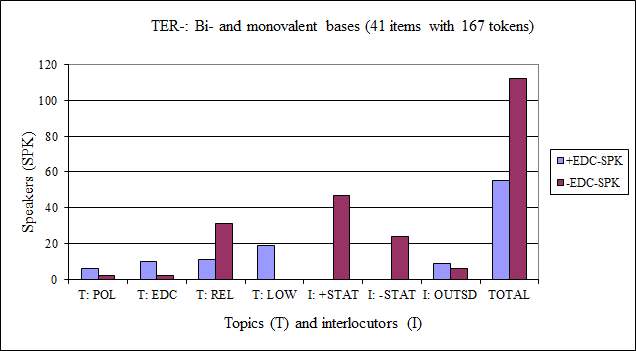
\includegraphics[scale=0.7]{./figures/Figure_3_1}
\begin{tikzpicture}
\begin{axis}[klugeaxis,title={\textscItal{ter}-: Bi- and \isi{monovalent} bases (41 items with 167 tokens)}]
\addplot[klugedots]	coordinates {(1,6)(2,10)(3,11)(4,19)(5,0)(6,0)(7,9)(8,55)};
\addplot[klugelines] coordinates {(1,2)(2,2)(3,31)(4,0)(5,47)(6,24)(7,6)(8,112)};		
\legend{\textsc{+edc-spk},\textsc{-edc-spk}}
\end{axis}
\end{tikzpicture}
\caption[Token frequencies for {ter-}prefixed lexemes with bi- and \isi{monovalent} verbal bases by speakers, topics, and interlocutors\label{Figure_3.1}]{Token frequencies for \textscItal{ter-}prefixed lexemes with bi- and \isi{monovalent} verbal bases by speakers, topics, and interlocutors\label{Figure_3.1}}
\end{figure}


The data given in \tabref{Table_3.5} and \figref{Figure_3.1} shows that for the 43 \textscItal{ter-}prefixed lexemes, most tokens (143/167 – 86\%) can be explained in terms of speaker education levels, topics, and/or role-relations between the speakers and their interlocutors; this total includes 130/153 tokens (85\%) with \isi{bivalent} bases, and 13/14 tokens (93\%) with \isi{monovalent} bases.


Only 55/167 tokens (33\%) were produced by better-educated speakers (\textsc{+edc-spk}) while most tokens (112/167 – 67\%) were produced by less-educated speakers (\textsc{-edc-spk}). The \textsc{+edc-spk} produced half of their tokens (27/55 – 49\%) during discussions about \textsc{high} topics, that is, political, educational or religious affairs (\textsc{pol}, \textsc{edc} and \textsc{rel}, respectively). Another 19 tokens (35\%) occurred during conversations with fellow-Papuans (both \textsc{+stat} and \textsc{-stat} speakers) about \textsc{low} topics. The remaining nine tokens (16\%) occurred while conversing with an outsider, namely the author (\textsc{outsd}).



The \textsc{-edc-spk} produced most of their tokens (47/112 – 42\%) while discussing \textsc{low} topics with \textsc{+stat} speakers (47 tokens). Another 35/112 tokens (31\%) were produced during discussions about \textsc{high} topics, while 6/112 tokens (5\%) occurred during conversations with the author. The remaining 24/112 tokens (21\%) occurred when \textsc{-edc-spk} discussed \textsc{low} topics with \textsc{-stat} Papuans, and therefore cannot be explained in terms of speaker education levels, topics, and/or role-relations. This total of 24 tokens refers to 14\% of all 167 \textscItal{ter-}tokens, including 23/153 tokens (15\%) with \isi{bivalent} bases and 1/14 tokens (7\%) with \isi{monovalent} bases.\footnote{As for the 21 hapaxes (17 with \isi{bivalent} and four with \isi{monovalent} bases), 18 appear to be conditioned by the variables of speaker education levels, topics, and/or role-relations, and therefore seem to be code-switches with Indonesian. This leaves only three hapaxes (with \isi{bivalent} bases) that are unaccounted for in terms of language external factors and that might result from a productive derivation process. For three hapaxes, P=0.0180 as opposed to P=0.1257 for 21 hapaxes (N=167).}


\subsubsection[Summary and conclusions]{Summary and conclusions}\label{Para_3.1.2.5}
For most of the derived verbs with \isi{bivalent} bases, the data suggests a productive form-function relationship between the derived lexemes and their bases. This conclusion is based on four observations: (1) the valency-decreasing or -reducing function of \textscItal{ter-} of removing or downplaying agent-like participants, (2) the transparent form-function relationships between derived lexemes and bases, (3) the large number of low frequency words and small number of high frequency words, and (4) the relative token frequencies with most bases having higher frequencies than the affixed lexemes.



For the prefixed verbs with \isi{monovalent} bases, the derivation process also seems to be productive, given (1) the transparent form-function relationships between derived lexemes and bases, (2) the comparatively large number of low frequency words and small number of high frequency words, and (3) the relative token frequencies with most bases having higher frequencies than the affixed lexemes. However, the low type frequency, with only five derived verbs, suggests that \textscItal{ter-}prefixation of \isi{monovalent} bases plays a minor role.



As for the speech situations during which the derived lexemes occurred, a sizable number of verbs with \isi{bivalent} bases cannot be explained in terms of pertinent variables of the \isi{communicative event}. Most tokens, however, including those with \isi{bivalent} bases, seem to be conditioned by the variables of speaker education levels, topics, and/or role-relations and therefore are best explained as code-switches with Indonesian.



These findings suggest that in Papuan Malay \textscItal{ter-}\isi{affixation} is a productive process to derive \isi{monovalent} verbs that denote accidental or unintentional actions. The degree of productivity appears to be limited, however, given that most of the attested tokens are best explained as code-switches with Indonesian.


\subsection{Suffix \textitbf{-an}\textitbf{g} ‘\textsc{pat}’}\label{Para_3.1.3}

Affixation with \textitbf{-ang} ‘\textsc{pat}’ typically derives nominals from verbal bases. The derived nouns denote the patient or result of the action, event, or state specified by the \isi{verbal base}, as illustrated in (\ref{Example_3.10}). Some lexical items are also derived from nominal and \isi{numeral} bases. The derivation process seems to be productive in Papuan Malay to some degree, as discussed below.


\ea
\label{Example_3.10}
\gll {\bluebold{pake–ang}} {itu} {basa} {smua}\\ %
 use–\textsc{pat}  \textsc{d.dist}  be.wet  all\\
\glt 
‘all those \bluebold{clothes} were wet’ \textstyleExampleSource{[080917-008-NP.0139]}
\z


Suffix \textitbf{-ang} is a reflex of Proto-\ili{Malayic} *\textitbf{-}\textscItal{a}\textitbf{n}, which “was a noun-forming suffix occurring on the basis of VTRs and denoting the goal or result of an act” \citep[174]{Adelaar.1992}. In Standard Malay, when affixed to \isi{monovalent} bases, the suffix designates “something that has the quality of” the \isi{monovalent} base, while with transitive bases it denotes the “goal or result of an action, or place where the action takes place” or “the instrument” (\citeyear*[172–173]{Adelaar.1992}). As for the \ili{eastern Malay varieties}, the suffix is only mentioned for \ili{Ambon Malay}. Also realized as \textitbf{-ang}, it “refers to the object of the transitive \isi{verb} or an instrument used in an act of V” \citep[106]{vanMinde.1997}. It is left unclear, however, whether and to what degree the \ili{Ambon Malay} suffix is productive. These observations are again an indication of the distinct history of Papuan Malay vis-à-vis the other Malay varieties, discussed in §\ref{Para_1.8}. Moreover, the similarities between Papuan Malay and \ili{Ambon Malay} reflect the link between both speech communities, also discussed in §\ref{Para_1.8}.


The corpus contains 84 nouns (441 tokens) suffixed with \textitbf{-}\textitbf{ang}:\footnote{The 84 nouns include 28 hapaxes (P=0.0635); the 69 nouns with verbal bases include 23 hapaxes (P=0.0571); the 15 nouns with nominal or \isi{numeral} bases include five hapaxes (P=0.1316).}


%\setcounter{itemize}{0}
\begin{enumerate}
\item 
Nouns with verbal bases (69 items with 403 tokens)
\item 
Nouns with nominal or \isi{numeral} bases (15 items with 38 tokens)
\end{enumerate}

The corpus also includes 28 formally complex words that have non-comp\-os\-ition\-al semantics, such as \textitbf{kasiang} ‘pity’, \textitbf{lapangang} ‘field’, or \textitbf{grakang} ‘movement’.



Suffixed items with verbal bases are examined in §\ref{Para_3.1.3.1}, and those with nominal bases in §\ref{Para_3.1.3.2}. Variables of the \isi{communicative event} that may impact the use of \textitbf{-ang} are explored in §\ref{Para_3.1.3.3}. The main findings on suffix \textitbf{-ang} are summarized and evaluated in §\ref{Para_3.1.3.4}.


\subsubsection[Suffixed items derived from verbal bases]{Suffixed items derived from verbal bases}\label{Para_3.1.3.1}

The corpus contains 69 \textitbf{-ang}{}-suffixed items (with 403 tokens) with verbal bases, including bases such as \isi{bivalent} \textitbf{pake} ‘use’, \isi{monovalent} dynamic \textitbf{jalang} ‘walk’, or \isi{monovalent} stative \textitbf{dulu} ‘be prior’. Affixation with \textitbf{-ang} typically derives nouns that denote the object of the action, event, or state indicated by the \isi{verbal base}.



Derived words with token frequencies of five or more are listed in \tabref{Table_3.6}. Most of the affixed lexemes are low frequency words (63 lexemes, attested with less than 20 tokens). Moreover, the token frequencies for the respective bases are (much) higher for most of the derived words (64 lexemes). While all 69 derived lexemes are structurally nouns, three of them have other than nominal functions in their actual uses: \textitbf{jualang} ‘merchandise’, \textitbf{duluang} ‘be prior’, and \textitbf{latiang} ‘practice'; illustrations are provided in (\ref{Example_3.13}) to (\ref{Example_3.15}).



Seven of the 69 lexemes were tentatively classified as borrowings from \ili{Standard Indonesian} (SI-borrowings) (for more details see language internal factor (\ref{List_3.1.f}) in §\ref{Para_3.1.1}, p. \pageref{List_3.1.f}). As their token frequencies are four or less, they are not included in \tabref{Table_3.6}.

\begin{table}
\caption{Affixation with \textitbf{-ang} of verbal bases}\label{Table_3.6}
\setlength{\tabcolsep}{0.6mm}
\begin{tabularx}{\textwidth}{llllrr}
\lsptoprule
 \multicolumn{1}{c}{BW} & \multicolumn{1}{c}{Gloss} & \multicolumn{1}{c}{Item} & \multicolumn{1}{c}{Gloss} & \multicolumn{1}{c}{\textitbf{-ang} \#} &  \multicolumn{1}{c}{BW \#}\\

\midrule

\textitbf{makang} & ‘eat’ & \textitbf{makangang} & ‘food’ &  57 &  414\\

\textitbf{pake} & ‘use’ & \textitbf{pakeang} & ‘clothes’ &  38 &  218\\

\textitbf{dulu} & ‘be prior’ & \textitbf{duluang} & ‘be prior to others’ &  29 &  351\\

\textitbf{bagi} & ‘divide’ & \textitbf{bagiang} & ‘part’ &  28 &  63\\

\textitbf{pikir} & ‘think’ & \textitbf{pikirang} & ‘thought’ &  23 &  102\\

\textitbf{uji} & ‘examine’ & \textitbf{ujiang} & ‘examination, examine’ &  21 &  1\\

\textitbf{lati} & ‘practice’ & \textitbf{latiang} & ‘practice’ &  17 &  3\\

\textitbf{kubur} & ‘burry’ & \textitbf{kuburang} & ‘grave’ &  14 &  8\\

\textitbf{atur} & ‘arrange’ & \textitbf{aturang} & ‘regulation’ &  8 &  24\\

\textitbf{ikat} & ‘tie up’ & \textitbf{ikatang} & ‘tie’ &  8 &  14\\

\textitbf{jual} & ‘sell’ & \textitbf{jualang} & ‘merchandise, sell’ &  8 &  14\\

\textitbf{turung} & ‘descend’ & \textitbf{turungang} & ‘descendant’ &  8 &  192\\

\textitbf{ulang} & ‘repeat’ & \textitbf{ulangang} & ‘\isi{repetition}’ &  8 &  16\\

\textitbf{bantu} & ‘help’ & \textitbf{bantuang} & ‘help’ &  7 &  34\\

\textitbf{alas} & ‘put down as base’ & \textitbf{alasang} & ‘reason’ &  6 &  7\\

\textitbf{bangun}\textitbf{g} & ‘build’ & \textitbf{bangungan}\textitbf{g} & ‘building’ &  6 &  25\\

\textitbf{libur} & ‘have vacation’ & \textitbf{liburang} & ‘vacation’ &  6 &  10\\

\textitbf{campur} & ‘mix’ & \textitbf{campurang} & ‘mixture’ &  5 &  5\\

\textitbf{jalang} & ‘walk’ & \textitbf{jalangang} & ‘route’ &  5 &  485\\

\textitbf{lapor} & ‘report’ & \textitbf{laporang} & ‘report’ &  5 &  14\\

\textitbf{tulis} & ‘write’ & \textitbf{tulisang} & ‘writing’ &  5 &  12\\

\lspbottomrule
\end{tabularx}
\end{table}

Affixing verbal bases with \textitbf{-ang} typically derives nouns that denote the object of the action specified by the \isi{verbal base}. The suffixed nouns include patients such as \textitbf{makangang} ‘that which is eaten’ or ‘food’, or results such as \textitbf{bagiang} ‘that which is divided’ or ‘part’. “Objective nominalization” that derives “nouns designating the result, or the typical or ‘cognate’ object of an action” has also been observed for other languages \citep[340]{Comrie.2007}. This polysemy can be explained in terms of a “domain shift” in that “one may go from one semantic domain to another, related one, and thus derive new interpretations” {\citep[221]{Booij.2007}}. Hence, suffix \textitbf{-ang} is glossed as ‘\textsc{pat}’ (‘patient’) in the sense of ‘patients or results which are \textsc{base}{}-ed’.


Two derived nouns together with their bases are given in context: \textitbf{makangang} ‘food’ with its \isi{bivalent} base \textitbf{makang} ‘eat’ in (\ref{Example_3.11}), and \textitbf{jalangang} ‘route’ with its \isi{monovalent} base \textitbf{jalang} ‘walk’ in (\ref{Example_3.12}).


\newpage
\begin{styleExampleTitle}
{Suffix \textitbf{-ang}: Semantics of verbal bases and derived lexemes}
\end{styleExampleTitle}

\ea
\label{Example_3.11}
\gll {maytua} {bilang,} {\bluebold{makang}} {karna} {\bluebold{makang–ang}} {suda} {masak}\\ %
 wife  say  eat  because  eat–\textsc{pat}  already  cook\\
\glt 
‘(my) wife said, ``\bluebold{eat}, because the \bluebold{food} has already been cooked''’ \textstyleExampleSource{[080919-004-NP.0039]}
\z

\ea
\label{Example_3.12}
\gll {{trus}} {kitong} {dua} {{pulang,}} {{sampe}} {di} {\bluebold{jalang–ang}} {sa} {istirahat,}\\ %
 {next}  \textsc{1pl}  two  {go.home}  {reach}  at  walk–\textsc{pat}  \textsc{1sg}  rest\\
\gll  de  {bilang,}  {kitong}  dua  {\bluebold{jalang}}  {suda!}\\
 \textsc{3sg}  {say}  {\textsc{1pl}}  two  {walk}  {already}\\
\glt 
‘and then we two went home, on the \bluebold{way} I rested, he said, ``let the two of us \bluebold{walk} (on)!''’ \textstyleExampleSource{[081015-005-NP.0036]}
\z


Some of the suffixed items, listed in \tabref{Table_3.6}, differ from the other suffixed items, as for example \textitbf{jual-ang} ‘sell-\textsc{pat}’ and \textitbf{dulu-ang} ‘be.prior-\textsc{pat}’. Suffixed with \textitbf{-ang}, these items are structurally nouns. In a sentence, however, \textitbf{jualang} also functions as the \isi{verb} ‘sell’ in the same way as its base \textitbf{jual} ‘sell’, as shown in (\ref{Example_3.13}). Likewise \textitbf{duluang} ‘be.prior-\textsc{pat}’ in (\ref{Example_3.14}) is used in the same way as its base \textitbf{dulu} ‘be prior’ in (\ref{Example_3.15}).



\begin{styleExampleTitle}
%\caption
{Suffix \textitbf{-ang}: Verbal reading of derived lexemes}
\end{styleExampleTitle}

\ea
\label{Example_3.13}
\gll {mama} {saya} {pergi} {\bluebold{jual}} {pinang,} {sa} {pu} {mama} {\bluebold{jual–ang}}\\ %
 mother  \textsc{1sg}  go  sell  betel.nut  \textsc{1sg}  \textsc{poss}  mother  sell–\textsc{pat}\\
\gll {pinang}\\
 {betel.nut}\\
\glt 
‘my mother went to \bluebold{sell} betel nuts, my mother \bluebold{sells} betel nuts’ \textstyleExampleSource{[081014-014-NP.0002]}
\z

\ea
\label{Example_3.14}
\gll {nanti} {kam} {dari} {blakang,} {bapa} {\bluebold{dulu–ang}}\\ %
 very.soon  \textsc{2pl}  from  backside  father  be.prior–\textsc{pat}\\

\glt
[About an upcoming official meeting:] ‘then you two (go in) second, (and) the gentleman \bluebold{(goes) ahead}’ \textstyleExampleSource{[081011-001-Cv.0199]}

\z
\ea
\label{Example_3.15}
\gll {dua} {orang} {\bluebold{dulu}}\\ %
 two  person  be.prior\\
\glt
[About the number of potential nominees for the upcoming local election:] ‘two people \bluebold{(go) ahead}’ \textstyleExampleSource{[080919-001-Cv.0065]}
\z

\subsubsection[Suffixed items derived from nominal or {numeral} bases]{Suffixed items derived from nominal or {numeral} bases}\label{Para_3.1.3.2}
The corpus contains 13 \textitbf{-ang}{}-suffixed lexemes with nominal bases (36 tokens) and two derived lexemes with \isi{numeral} bases (2 tokens), as listed in \tabref{Table_3.7}. In most cases, the bases and the derived nouns differ in their semantics. In some cases, the affixed nouns designate a magnification of the base, such as \textitbf{laut} ‘sea’ and \textitbf{lautang} ‘ocean’, or \textitbf{ruang} ‘room’ and \textitbf{ruangang} ‘large room’. In some cases, the meanings of the derived nouns are an extension of the meanings of their bases with suffix \textitbf{-ang} having a generalizing function, as for instance \textitbf{ana} ‘child’ and \textitbf{anaang} ‘offspring’, or \textitbf{musim} ‘season’ and \textitbf{musimang} ‘each season’. In yet other cases, the affixed nouns have unpredictable meanings compared to the semantics of their bases, such as \textitbf{rambut} ‘hair’ and \textitbf{rambutang} ‘rambutan’, or \textitbf{obat} ‘medicine’ and \textitbf{obatang} ‘magic spell’. And in a few cases, the base and the derived \isi{noun} have the same semantics, as in \textitbf{pasang} ‘pair’ and \textitbf{pasangang} ‘pair’ or \textitbf{pangkal} ‘base’ and \textitbf{pangkalang} ‘base’.



All 13 derived lexemes are low frequency words, attested with less than 20 tokens. Moreover, the token frequencies for the respective bases are (much) higher for most of the derived words (10 lexemes); for one lexeme, the base is unattested in the corpus, although it does exist. Four of the 15 derived nouns were tentatively classified as SI-borrowings; in \tabref{Table_3.7} these items are underlined (for more details see language internal factor (\ref{List_3.1.f}) in §\ref{Para_3.1.1}, p. \pageref{List_3.1.f}).

\begin{table}

\caption{Affixation with \textitbf{-ang} of nominal and \isi{numeral} bases}\label{Table_3.7}
\begin{tabularx}{\textwidth}{lXXXrr}
\lsptoprule

 \multicolumn{1}{c}{BW} & \multicolumn{1}{c}{Gloss} & \multicolumn{1}{c}{Item} & \multicolumn{1}{c}{Gloss} & \multicolumn{1}{c}{\textitbf{-ang} \#} & \multicolumn{1}{c}{ BW \#}\\

\midrule
\textitbf{bayang} & ‘image’ & \textitbf{bayangang} & ‘shadow’ &  6 &  2\\

\textitbf{ana} & ‘child’ & \textitbf{anaang} & ‘offspring’ &  4 &  741\\

\textitbf{tingkat} & ‘floor’ & \textitbfUndl{tingkatang} & ‘level’ &  4 &  5\\

\textitbf{hukum} & ‘law’ & \textitbf{hukumang} & ‘punishment’ &  4 &  3\\

\textitbf{rambut} & ‘hair’ & \textitbf{rambutang} & ‘rambutan’ &  3 &  23\\

\textitbf{obat} & ‘medicine’ & \textitbf{obatang} & ‘magic spell’ &  3 &  9\\

\textitbf{pasang} & ‘pair’ & \textitbf{pasangang} & ‘pair’ &  3 &  2\\

\textitbf{laut} & ‘sea’ & \textitbf{lautang} & ‘ocean’ &  2 &  68\\

\textitbf{pinggir} & ‘border’ & \textitbfUndl{pinggirang} & ‘edges’ &  2 &  23\\

\textitbf{ruang} & ‘room’ & \textitbf{ruangang} & ‘large room’ &  2 &  3\\

\textitbf{kandung} & ‘womb’ & \textitbfUndl{kandungang} & ‘womb’ &  1 &  8\\

\textitbf{musim} & ‘season’ & \textitbfUndl{musimang} & ‘each season’ &  1 &  5\\

\textitbf{pangkal} & ‘base’ & \textitbf{pangkalang} & ‘base’ &  1 &  0\\

\textitbf{pulu} & ‘tens’ & \textitbf{puluang} & ‘tens’ &  1 &  78\\

\textitbf{ratus} & ‘hundreds’ & \textitbf{ratusang} & ‘hundreds’ &  1 &  34\\

\lspbottomrule
\end{tabularx}
\end{table}

The data listed in \tabref{Table_3.7} shows that most of the nominal bases and affixed nouns differ in their semantics. The magnifying function of suffix \textitbf{-ang} is illustrated in (\ref{Example_3.16}) and (\ref{Example_3.17}), the generalizing function in (\ref{Example_3.18}), and its unpredictable semantics in (\ref{Example_3.19}) and (\ref{Example_3.20}).


The magnifying function of \textitbf{-ang} is demonstrated with \textitbf{laut} ‘sea’ in (\ref{Example_3.16}) and \textitbf{lautang} ‘ocean’ in (\ref{Example_3.17}). While \textitbf{laut} refers to the ‘sea’ close to the coast, \textitbf{lautang} denotes the open and deep ‘ocean’ off the coast.

\newpage

\begin{styleExampleTitle}
{Suffix \textitbf{-ang}: Magnifying function}
\end{styleExampleTitle}

\ea
\label{Example_3.16}
\gll {dong} {dua} {pergi} {mancing} {di} {\bluebold{laut}}\\ %
 \textsc{3pl}  two  go  fish.with.rod  at  sea\\
\glt 
‘the two of them went fishing on the \bluebold{sea}’ \textstyleExampleSource{[081109-005-JR.0005]}
\z
\ea
\label{Example_3.17}
\glll {banyak} {mati} {\ldots} {di} {pulow{\Tilde}pulow} {banyak} {mati} {di} \bluebold{laut–ang}\\ %
{} {} {} {} {} {} {} {} {sea–\textsc{pat}}\\
 many  die {}   at  \textsc{rdp}{\Tilde}island  many  die  at  ocean\\
\glt ‘many died {\ldots} on the islands, many died on the (open) \bluebold{ocean}’ \textstyleExampleSource{[081029-002-Cv.0025]}
\z
%\todo[inline]{Please check this example.}

The generalizing function of \textitbf{-ang} is illustrated with \textitbf{ana} ‘child’ and \textitbf{anaang} ‘offspring’ in (\ref{Example_3.18}).



\begin{styleExampleTitle}
{Suffix \textitbf{-ang}: Generalizing function}
\end{styleExampleTitle}
\ea
\label{Example_3.18}
\gll {kalo} {{mo}} {antar} {{\bluebold{ana}}} {{\bluebold{prempuang}}} {ke} {\bluebold{ana}} {{\bluebold{laki{\Tilde}laki}}} {{\ldots}} {kitorang}\\ %
 if  {want}  bring  {child}  {woman}  to  child  {\textsc{rdp}{\Tilde}husband}  {}  \textsc{1pl}\\
 
 \glll {itu}  {harus}  {\ldots}  {bawa}  \bluebold{ana–ang}  {pinang}  \bluebold{ana–ang}  {sagu}\\
 {} {} {} {} child–\textsc{pat} {} child–\textsc{pat} {} \\
  {\textsc{d.dist}} {have.to} {}   {bring}  {offspring}  {betel.nut}  {offspring}  {sago}\\
\glt 
[About wedding preparations:] ‘if we want to bring our \bluebold{daughter} to (their) \bluebold{son} {\ldots} we have to {\ldots} bring betel nut \bluebold{seedlings} (and) sago \bluebold{seedlings}’ (Lit. ‘female/male \bluebold{child}; betel nut/sago \bluebold{offspring}’) \textstyleExampleSource{[081110-005-CvPr.0055-0057]}
\z
%\todo[inline]{Please check this example.}


In some cases, the semantics of the affixed nouns are unpredictable, although a connection between the base word and the derived word can still be seen. This is demonstrated with \textitbf{rambut} ‘hair’ in (\ref{Example_3.19}) and \textitbf{rambutang} ‘rambutan’ in (\ref{Example_3.20}), which refers to the fruit of the rambutan tree (\textstyleChItalic{Nephelium lappaceum}). The leathery reddish skin of the fruit is covered with numerous hairy protuberances, which is depicted by the label \textitbf{rambut-ang} ‘hair-\textsc{pat}’.



\begin{styleExampleTitle}
{Suffix \textitbf{-ang}: Unpredictable semantics}
\end{styleExampleTitle}

\ea
\label{Example_3.19}
\gll {sa} {mo} {cuci} {de} {pu} {\bluebold{rambut}}\\ %
 \textsc{1sg}  want  wash  \textsc{3sg}  \textsc{poss}  hair\\
\glt 
‘I want to wash her \bluebold{hair}’ \textstyleExampleSource{[081025-001-CvHt.0006]}
\z

\ea
\label{Example_3.20}
\glll {di} {sini} {ada} {jambu} {di} {sini} {ada} {ada} \bluebold{rambut–ang}\\ %
 {} {} {} {} {} {} {} {} hair–\textsc{pat}\\
 at  \textsc{l.prox}  exist  rose.apple  at  \textsc{l.prox}  exist  exist  rambutan\\
\glt
‘here are rose apples, here are are \bluebold{rambutan}’ \textstyleExampleSource{[081029-001-Cv.0006]}
\z
%\todo[inline]{Please check this example.}

\subsubsection[Variables of the {communicative event}]{Variables of the communicative event}\label{Para_3.1.3.3}

To further investigate the issue of productivity of \textitbf{-ang} in Papuan Malay, a domain analysis was conducted which focused on the variables of speaker education levels, topics, and/or role-relations (for details see ``Language external factors'' in §\ref{Para_3.1.1}, p. \pageref{List_3.2}). In all, 84 items suffixed with \textitbf{-ang}, totaling 441 tokens, were investigated:


\begin{itemize}
\item 
69 suffixed items derived from verbal bases (403 tokens)

\item 
15 suffixed items derived from nominal or \isi{numeral} bases (38 tokens)

\end{itemize}

For the 84 suffixed lexemes, 352/441 tokens (80\%) can be accounted for in terms of speaker education levels, topics, and/or role-relations. The remaining 89/441 tokens (20\%) occurred when less-educated speakers (\textsc{-edc-spk}) talked with fellow-Papuans of equally low social standing (\textsc{-stat}) about \textsc{low} topics.\footnote{As mentioned under Factor 3 ``Relationships between interlocutors'' in §\ref{Para_1.5.1} (p. \pageref{Item_1.3}), all of the recorded less-educated speakers belong to the group of Papuans with lower social status (\textsc{-stat}), while the recorded Papuans with higher social status (\textsc{+stat}), such as teachers, government officials, or pastors, are all better educated.} (See \tabref{Table_3.8} and \figref{Figure_3.2}.)



That is, a considerable number of tokens (20\%) cannot be explained in terms of these variables of the \isi{communicative event}. Therefore, it cannot be concluded that the respective lexemes are code-switches with Indonesian. This total of 89/441 tokens (20\%) includes 80/403 tokens (20\%) with verbal bases and 9/38 tokens (24\%) with nominal or \isi{numeral} bases. The vast majority of \textitbf{-ang}{}-suffixed tokens (352/441 – 80\%), however, seem to be conditioned by variables of the \isi{communicative event}.



As for the rather high number of unaccounted tokens with nominal or \isi{numeral} bases (9/38 – 24\%), one observation is made. Four of the nine tokens refer to the same lexeme produced by the same speaker during three conversations about the same topic, namely the death of a young mother. This speaker has a reputation of speaking incoherently due to his unsuccessful attempts to approximate \ili{Standard Indonesian}. Excluding these four tokens brings down the number of unaccounted lexemes to 15\% (5/34). If \isi{affixation} of nominal bases was a productive process, however, one would expect this percentage to be much higher. In turn, this finding does not support the conclusion that the suffixed lexemes with nominal or \isi{numeral} bases result from a productive derivation process. Instead, they seem to be code-switches with Indonesian.



The data presented in \tabref{Table_3.8} and \figref{Figure_3.2} is discussed in more detail below.

\begin{table}
\caption{Token frequencies for \textitbf{-ang}{}-suffixed lexemes with verbal, nominal, and \isi{numeral} bases by speakers, topics, and interlocutors (84 items)}\label{Table_3.8}

\begin{tabular}{lllllllll}
\lsptoprule

 & \multicolumn{4}{l}{ Topics (\textsc{top})} & \multicolumn{3}{l}{ Interlocutors (\textsc{ilct})} &  Tokens\\
\midrule
\multicolumn{9}{l}{Suffixed lexemes with verbal bases (69 items)}\\
\midrule
& \textsc{pol} & \textsc{edc} & \textsc{rel} & \textsc{low} & \textsc{+stat} & \textsc{-stat} & \textsc{outsd} &  Total\\

\textsc{+edc-spk} &  30 &  26 &  15 &  46 &  {}-{}-{}- &  {}-{}-{}- &  75 &  192\\

\textsc{-edc-spk} &  15 &  40 &  47 &  {}-{}-{}- &  26 &  \textstyleChBold{80} &  3 &  211\\

Subtotal &  45 &  66 &  62 &  46 &  26 &  \textstyleChBold{80} &  78 &  403\\
\midrule
\multicolumn{9}{l}{Suffixed lexemes with nominal and \isi{numeral} bases (15 items)}\\
\midrule

& \textsc{pol} & \textsc{edc} & \textsc{rel} & \textsc{low} & \textsc{+stat} & \textsc{-stat} & \textsc{outsd} &  Total\\

\textsc{+edc-spk} &  4 &  1 &  0 &  4 &  {}-{}-{}- &  {}-{}-{}- &  8 &  17\\

\textsc{-edc-spk} &  3 &  0 &  6 &  {}-{}-{}- &  1 &  \textstyleChBold{9} &  2 &  20\\

Subtotal &  7 &  1 &  6 &  4 &  1 &  \textstyleChBold{9} &  10 &  38\\
\midrule
\multicolumn{9}{l}{\textstyleChBold{TOTAL} (84 items)}\\
\midrule
& \textsc{pol} & \textsc{edc} & \textsc{rel} & \textsc{low} & \textsc{+stat} & \textsc{-stat} & \textsc{outsd} &  Total\\

\textsc{+edc-spk} &  34 &  27 &  15 &  50 &  {}-{}-{}- &  {}-{}-{}- &  83 &  209\\

\textsc{-edc-spk} &  18 &  40 &  53 &  {}-{}-{}- &  27 &  \textstyleChBold{89} &  5 &  232\\
\midrule
\textstyleChBold{Total} &  52 &  67 &  68 &  50 &  27 &  \textstyleChBold{89} &  88 &  \textstyleChBold{441}\\

\lspbottomrule
\end{tabular}
\end{table}
\begin{figure}
\centering
%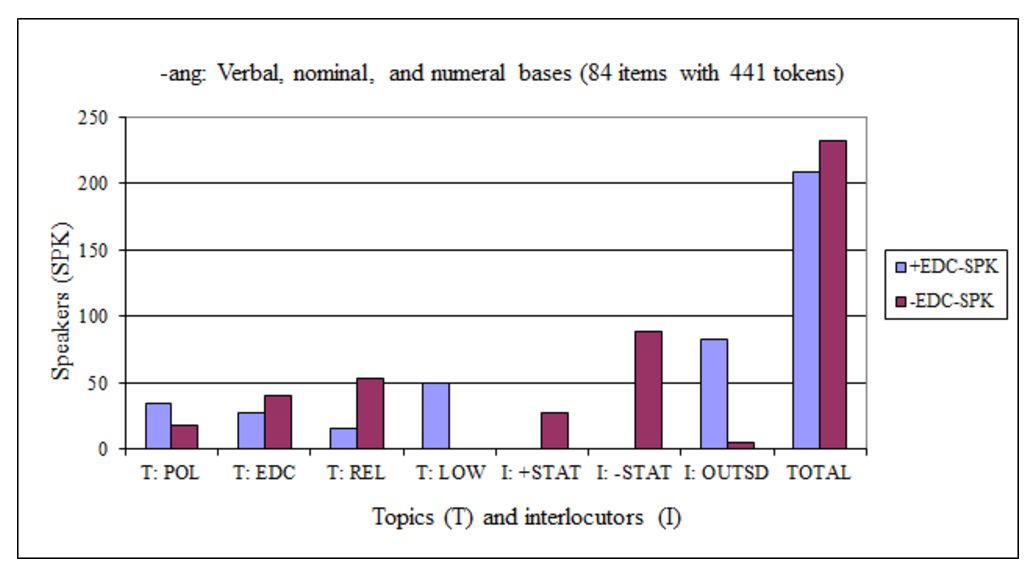
\includegraphics[scale=0.7]{./figures/Figure_3_2}
\begin{tikzpicture}
\begin{axis}[klugeaxis, y={}, height={.5\textheight}, title={\textitbf{-ang}: Verbal, nominal, and \isi{numeral} bases (84 items with 441 tokens)}]
\addplot[klugedots]	coordinates {(1,34)(2,27)(3,15)(4,50)(5,0)(6,0)(7,83)(8,209)};
\addplot[klugelines] coordinates {(1,18)(2,40)(3,53)(4,0)(5,27)(6,89)(7,5)(8,232)};		
\legend{\textsc{+edc-spk},\textsc{-edc-spk}}
\end{axis}
\end{tikzpicture}
\caption{Token frequencies for \textitbf{-ang}{}-suffixed lexemes with verbal, nominal, and \isi{numeral} bases by speakers, topics, and interlocutors\label{Figure_3.2}}
\end{figure}

The data given in \tabref{Table_3.8} and \figref{Figure_3.2} shows that for the 84 \textitbf{-ang}{}-suffixed lexemes, 352/441 tokens (80\%) can be explained in terms of speaker education levels, topics, and/or role-relations between the speakers and their interlocutors; this includes 323/403 tokens (80\%) with verbal bases, and 29/38 tokens (76\%) with nominal bases.


The better-educated speakers (\textsc{+edc-spk}) produced 209/441 tokens (47\%), while the less-educated speakers (\textsc{-edc-spk}) produced 232/441 (53\%) tokens.



In terms of topics (\textsc{top}), 187/441 tokens (42\%) occurred during conversations about \textsc{high} topics, that is, political, educational or religious affairs (\textsc{pol}, \textsc{edc} and \textsc{rel}, respectively). This includes 76/209 \textsc{+edc-spk} tokens (36\%) and 111/232 \textsc{-edc-spk} tokens (48\%). 
Another 88/441 tokens (20\%) were produced in conversations with an outsider, namely the author (\textsc{outsd}), including 83/209 \textsc{+edc-spk} tokens (40\%) and 5/232 \textsc{-edc-spk} tokens (0.2\%).



This leaves 166/441 tokens (38\%) that were produced when the interlocutors discussed \textsc{low} topics. This includes 50/166 \textsc{+edc-spk} tokens (30\%) and 116/166 \textsc{-edc-spk} tokens (70\%). The 116 \textsc{low} topic tokens produced by \textsc{-edc-spk} are distributed as follows. When conversing with \textsc{+stat} Papuans, 27 tokens were produced (that is, 27/232 \textsc{-edc-spk} tokens – 12\%). The remaining 89 tokens (that is, 89/232 \textsc{-edc-spk} tokens – 38\%) occurred when \textsc{-edc-spk} discussed \textsc{low} topics with \textsc{-stat} Papuans, and therefore cannot be explained in terms of speaker education levels, topics, and/or role-relations. This total of 89 tokens refers to 20\% of all 441 \textitbf{-ang} tokens. It includes 80/403 tokens (20\%) with verbal bases and 9/38 tokens (24\%) with nominal or \isi{numeral} bases.\footnote{As for the 28 hapaxes (23 with verbal bases, and five with nominal bases), 17 appear to be conditioned by the variables of speaker education levels, topics, and/or role-relations, and therefore are best explained as code-switches with Indonesian. This leaves 11 hapaxes that are unaccounted for in terms of language external factors and that might be the result of a productive \isi{word-formation} process. For 11 hapaxes, P=0.0249 as opposed to P=0.0635 for 28 hapaxes (N=441). The total of 11 hapaxes includes nine with verbal bases (P=0.0223) and two with nominal or \isi{numeral} bases (P=0.0526).}


\subsubsection[Summary and conclusions]{Summary and conclusions}\label{Para_3.1.3.4}

Suffix \textitbf{-ang} is polyfunctional in that it derives nouns from verbal, nominal, and \isi{numeral} bases. This polyfunctionality suggests that \isi{affixation} with \textitbf{-ang} is a somewhat productive process (see language internal factor (\ref{List_3.1.c}) in §\ref{Para_3.1.1}, p. \pageref{List_3.1.c}).



Concerning \textitbf{-ang}{}-\isi{affixation} of verbal bases, four other observations support this conclusion: (1) the transparent form-function relationship between the derived nouns and their respective bases, (2) the large number of low frequency words and small number of high frequency words, (3) the relative token frequencies with most bases having higher frequencies than the affixed lexemes, and (4) the low number of derived lexemes tentatively classified as SI-borrowings.



To a lesser extent, the same observations apply to \textitbf{-ang}{}-\isi{affixation} of nominal bases: (1) the form-function relationships between derived lexemes and bases is more or less transparent, (2) all derived lexemes are low frequency words, (3) most bases have higher token frequencies than the affixed lexemes, and (3) the number of derived lexemes tentatively classified as SI-borrowings is rather low. These findings suggest that \textitbf{-ang}{}-\isi{affixation} of nominal bases is also a somewhat productive process.



With respect to the speech situations during which the derived nouns occurred, the following patterns emerge. For affixed nouns with verbal bases, one fifth of the attested tokens cannot be accounted for in terms of pertinent variables of the \isi{communicative event}; that is, for these items there are no indications that they are code-switches with Indonesian. However, the vast majority of tokens with verbal bases (80\%) seem to be conditioned by the variables of speaker education levels, topics, and/or role-relations and are best explained as code-switches with Indonesian. The same applies to nouns with nominal bases for which most tokens also appear to be conditioned by the three mentioned variables of the \isi{communicative event}. Hence, these items are also best explained as code-switches with Indonesian.



These findings suggest that in Papuan Malay \textitbf{-ang}{}-\isi{affixation} is a productive process to derive nouns from verbal and nominal bases. The degree of productivity appears to be limited, however, as most tokens seem to be code-switches with Indonesian.


\subsection[Prefix {\PEN}- ‘\textsc{ag}’]{Prefix \textscItal{pe(n)}- ‘\textsc{ag}’}\label{Para_3.1.4}

Affixation with \textscItal{pe(n)}- ‘\textsc{ag}’ typically derives nominals from verbal bases. The derived nouns denote the agent or instrument of the action, event, or state specified by the \isi{verbal base}, as in (\ref{Example_3.21}). Some lexemes are also derived from nominal bases. The \isi{affixation} process appears to be marginally productive in Papuan Malay, at best, as discussed below.


\ea
\label{Example_3.21}
\gll {pokoknya} {orang} {\bluebold{pen–datang}} {pulang}\\ %
 the.main.thing.is  person  \textsc{ag}–come  go.home\\
\glt 
‘the main thing is (that) the \bluebold{strangers} return home’ (Lit. ‘\bluebold{the one who comes}’) \textstyleExampleSource{[081029-005-Cv.0048]}
\z


Suffix \textscItal{pe(n)-} is a reflex of Proto-\ili{Malayic} *\textitbf{p}\textscItal{an}\textitbf{-}, which “formed deverbal nouns that were used attributively, predicatively, and in prepositional phrases, and that had a nominal as head or subject. They denoted a purpose or instrument when prefixed to VDIs and VTRs. Moreover, *\textitbf{p}\textscItal{an}\textitbf{-} denoted an inclination or characteristic when prefixed to VSIs” \citep[193]{Adelaar.1992}. In Standard Malay, derived lexemes with a \isi{monovalent} base “denote a characteristic” while forms with a \isi{bivalent} base “usually denote an actor or instrument” or “a goal or result, or they form an abstract \isi{noun}. Furthermore \textitbf{pa}\textscItal{n}\textitbf{-} forms are used attributively, and, on the basis of VSIs, they can function as VSIs” (\citeyear*[183]{Adelaar.1992}).



In some of the \ili{eastern Malay varieties}, the prefix is also found. In \ili{Ambon Malay}, the prefix occurs but it is unproductive \citep[109]{vanMinde.1997}. In \ili{Manado Malay} \textitbf{paŋ-} also occurs and is productive (in addition, a unproductive form \textitbf{pa}\textsc{-} exists) \citep[18, 24]{Stoel.2005}. Likewise, in North Moluccan / \ili{Ternate Malay} \textitbf{pa(}\textscItal{n}\textitbf{)-} occurs, but its status is uncertain. While {\citet[4]{Voorhoeve.1983}} maintains that it “is no longer morphologically distinct”, \citet[30]{Litamahuputty.2012} states that the prefix is productive. In these varieties, the prefix usually denotes the actor or instrument of the event expressed by the base. In addition, however, some of prefixed forms can also receive a verbal reading, as discussed in more detail in §\ref{Para_3.1.4.2}.



The corpus contains 34 nouns (186 tokens) prefixed with \textscItal{pe(n)-}:\footnote{The 34 nouns include 11 hapaxes (P=0.0591); the 29 nouns with verbal bases include nine hapaxes (P=0.0588); the five nouns with nominal bases include two hapaxes (P=0.0606).}


\begin{enumerate}
\item 
Nouns with verbal bases (29 items with 153 tokens)
\item 
Nouns with nominal bases (five items with 33 tokens)
\
\end{enumerate}

The corpus also contains nine formally complex words with non-compositional semantics, such as \textitbf{peserta} ‘participant’ or \textitbf{panggayu} ‘(a/to) paddle’.



Before discussing \textscItal{pe(n)-}\isi{affixation} of verbal bases in §\ref{Para_3.1.4.2} and of nominal bases in §\ref{Para_3.1.4.3}, the \isi{allomorphy} of \textscItal{pe(n)-} is investigated in §\ref{Para_3.1.4.1}. Variables of the \isi{communicative event} that may impact the use of \textscItal{pe(n)-} are explored in §\ref{Para_3.1.4.4}. The main points on prefix \textscItal{pe(n)-} are summarized and evaluated in §\ref{Para_3.1.4.5}.


\subsubsection[Allomorphy of pe(n)-]{Allomorphy of \textscItal{pe(n)-}}\label{Para_3.1.4.1}

Prefix \textscItal{pe(n)-} has two allomorphs, \textitbf{pe(}\textscItal{n}\textitbf{)}\textitbf{-} and \textitbf{pa(}\textscItal{n}\textitbf{)}\textitbf{-} (small-caps \textscItal{n} represents the different realizations of the nasal). The allomorphs are not governed by phonological processes.



The form \textitbf{pe(}\textscItal{n}\textitbf{)}\textitbf{-}, in turn, has seven allomorphs that result from morphologically conditioned phonological rules. More specifically, they are conditioned by the word-initial segment of the base word, as shown in \tabref{Table_3.9}: /\textstyleChCharisSIL{pɛm-}/, /\textstyleChCharisSIL{pɛn-}/, /\textstyleChCharisSIL{pɛɲ-}/, \textstyleChCharisSIL{pɛŋ-}/, /\textstyleChCharisSIL{pɛ-}/, /\textstyleChCharisSIL{p-}/, and /\textstyleChCharisSIL{pl-}/. The prefix is realized as /\textstyleChCharisSIL{pɛm-}/ when the initial segment of the base is a bilabial stop. Onset voiced stops are retained, while voiceless stops are deleted. With onset bilabial /\textstyleChCharisSIL{m}/, the prefix is realized as /\textstyleChCharisSIL{pɛ-}/. With alveolar stops, the prefix is very commonly realized as /\textstyleChCharisSIL{pɛn-}/. Again, the onset voiced stop is retained, while the onset voiceless stop is deleted. Alternatively, however, the onset voiceless stop can also be retained, in which case the prefix is realized as /\textstyleChCharisSIL{pɛ-}/. With onset fricative /\textstyleChCharisSIL{s}/, the prefix is realized as /\textstyleChCharisSIL{pɛɲ-}/, with /\textstyleChCharisSIL{s}/ being deleted. With onset palato-alveolar affricates, \textitbf{pe(}\textscItal{n}\textitbf{)}\textitbf{-} is realized as /\textstyleChCharisSIL{pɛn-}/. With onset rhotic /r/, the affix is realized as /\textstyleChCharisSIL{pɛ-}/. With onset velar stops and onset vowels, the prefix is realized as /\textstyleChCharisSIL{pɛŋ-}/. Finally, when prefixed to \textitbf{ajar} ‘teach’, \textitbf{pe(}\textscItal{n}\textitbf{)}\textitbf{-} is realized as /\textstyleChCharisSIL{pl-}/.

\begin{table}
\caption[Realizations of allomorph \textitbf{pe(n)-}]{Realizations of allomorph \textitbf{pe(}\textscItal{n}\textitbf{)}\textitbf{-}}\label{Table_3.9}


\begin{tabular}{lll}
\lsptoprule

 \multicolumn{1}{c}{\textitbf{pe(}\textscItal{n}\textitbf{)-}base} & \multicolumn{1}{c}{Orthogr.} &  \multicolumn{1}{c}{Gloss}\\

\midrule
/\textstyleChCharisSIL{pɛm}–\textstyleChCharisSIL{bantu}/ & \textitbf{pembantu} & ‘house helper’\\

/\textstyleChCharisSIL{pɛm}–\textstyleChCharisSIL{pili}/ & \textitbf{pemili} & ‘voter’\\

/\textstyleChCharisSIL{pɛ}–\textstyleChCharisSIL{muda}/ & \textitbf{pemuda} & ‘youth’\\

/\textstyleChCharisSIL{pɛn}–\textstyleChCharisSIL{dataŋ}/ & \textitbf{pendatang} & ‘newcomer’\\

/\textstyleChCharisSIL{pɛn}–\textstyleChCharisSIL{tumpaŋ}/ & \textitbf{penumpang} & ‘passenger’\\

/\textstyleChCharisSIL{pɛ}–\textstyleChCharisSIL{tugas}/ & \textitbf{petugas} & ‘official’\\

/\textstyleChCharisSIL{pɛɲ}–\textstyleChCharisSIL{sakit}/ & \textitbf{penyakit} & ‘disease’\\

/\textstyleChCharisSIL{pɛn}–\textstyleChCharisSIL{tʃuri}/ & \textitbf{pencuri} & ‘thief, to steal (\textsc{emph})’\\

/\textstyleChCharisSIL{pɛn}–\textstyleChCharisSIL{dʒaga}/ & \textitbf{penjaga} & ‘guard’\\

/\textstyleChCharisSIL{pɛ}–\textstyleChCharisSIL{rɛntʃana}/ & \textitbf{perencana} & ‘planner’\\

/\textstyleChCharisSIL{pɛŋ–acara}/ & \textitbf{pengacara} & ‘master of ceremony’\\

/\textstyleChCharisSIL{pɛŋ}–\textstyleChCharisSIL{ganti}/ & \textitbf{pengganti} & ‘replacement’\\

/\textstyleChCharisSIL{pl}–\textstyleChCharisSIL{adʒar}/ & \textitbf{plajar} & ‘teacher’\\

\lspbottomrule
\end{tabular}
\end{table}

The allomorph \textitbf{pa(}\textscItal{n}\textitbf{)}\textitbf{-} occurs considerably less frequently. Attested are only the four items listed in \tabref{Table_3.10} with a total of 18 \textitbf{pa(}\textscItal{n}\textitbf{)}\textitbf{-} tokens. Form \textitbf{pa(}\textscItal{n}\textitbf{)}\textitbf{-} has two attested allomorphs: /\textstyleChCharisSIL{pan-}/ and /\textstyleChCharisSIL{pa-}/. The phonological processes involved in the \isi{allomorphy} are the same as those for \textitbf{pe(}\textscItal{n}\textitbf{)}\textitbf{-}, discussed above. For two of the items, the prefix is alternatively realized as allomorph \textitbf{pe(}\textscItal{n}\textitbf{)}\textitbf{-}. Therefore, for each item the token frequencies for \textitbf{pa(}\textscItal{n}\textitbf{)}\textitbf{-} and for \textitbf{pe(}\textscItal{n}\textitbf{)}\textitbf{-} are given. If the prefix is realized with /\textstyleChCharisSIL{pɛ(}\textsc{n}\textstyleChCharisSIL{)-}/ in a greater number of tokens than with /\textstyleChCharisSIL{pa(}\textsc{n}\textstyleChCharisSIL{)-}/, then its orthographic representation is \textscItal{pe(n)-} as in \textitbf{pencuri} ‘thief, steal (\textsc{emph})’.

\begin{table}
\caption[Realizations of allomorph \textitbf{pa(n)-}]{Realizations of allomorph \textitbf{pa(}\textscItal{n}\textitbf{)}\textitbf{-}}\label{Table_3.10}


\begin{tabularx}{\textwidth}{llXll}
\lsptoprule

 \textitbf{pa(}\textscItal{n}\textitbf{)}\textitbf{{}-}base & Orthogr. & \multicolumn{1}{c}{Gloss} & \textitbf{pa(}\textscItal{n}\textitbf{)}\textitbf{-} \# &  \textitbf{pe(}\textscItal{n}\textitbf{)}\textitbf{-} \#\\
\midrule
/\textstyleChCharisSIL{pa}–\textstyleChCharisSIL{malas}/ & \textitbf{pamalas} & ‘listless person, be very listless’ &  12 &  2\\

/\textstyleChCharisSIL{pan}–\textstyleChCharisSIL{diam}/ & \textitbf{pandiam} & ‘taciturn person, be very quiet’ &  2 &  0\\

/\textstyleChCharisSIL{pan}–\textstyleChCharisSIL{takut}/ & \textitbf{panakut} & ‘coward, be very fearful (of)’ &  3 &  0\\

/\textstyleChCharisSIL{pan}–\textstyleChCharisSIL{tʃuri}/ & \textitbf{pencuri} & ‘thief, steal (\textsc{emph})’ &  1 &  11\\

\lspbottomrule
\end{tabularx}
\end{table}

In realizing the prefix typically as \textitbf{pe(}\textscItal{n}\textitbf{)}\textitbf{-} rather than as \textitbf{pa(}\textscItal{n}\textitbf{)}\textitbf{-}, Papuan Malay differs from other \ili{eastern Malay varieties} such as \ili{Ambon Malay} \citep[109]{vanMinde.1997}, \ili{Manado Malay} \citep[23]{Stoel.2005}, and North Moluccan / \ili{Ternate Malay} (\citealt[4]{Voorhoeve.1983}; \citealt[30]{Litamahuputty.2012}). In these varieties the prefix is always realized as \textitbf{pa(}\textscItal{n}\textitbf{)}\textitbf{-}. Instead, the \textscItal{pe(n)-}prefixed items have more resemblance with the corresponding items in \ili{Standard Indonesian} where the prefix is realized as \textitbf{pe(}\textscItal{n}\textitbf{)}\textitbf{-}. This is again an indication of the distinct history of Papuan Malay vis-à-vis the other \ili{eastern Malay varieties}, discussed in §\ref{Para_1.8}.


\subsubsection[Prefixed items derived from verbal bases]{Prefixed items derived from verbal bases}\label{Para_3.1.4.2}

The corpus includes 29 \textscItal{pe(n)-} prefixed nouns (with 153 tokens) with verbal bases, listed in  \tabref{Table_3.11a} and \tabref{Table_3.11b}. Included are items with biverbal bases such as \textitbf{curi} ‘steal’, \isi{monovalent} dynamic bases such as \textitbf{duduk} ‘sit’, or \isi{monovalent} stative bases such as \textitbf{muda} ‘be young’. The \isi{affixation} process derives nouns that designate the subject of the action, event, or state specified by the \isi{verbal base}.



All but one of the derived words are low frequency words (28 lexemes, attested with less than 20 tokens). In addition, the token frequencies for the respective bases are (much) higher for most of the derived words (24 lexemes). While the 29 prefixed items are structurally nouns, four of them also have verbal functions in their actual uses: \textitbf{pamalas} ‘listless person, be very listless’, \textitbf{pandiam} ‘taciturn person, be very quiet’, \textitbf{panakut} ‘coward, be very fearful (of)’, and \textitbf{pencuri} ‘thief, steal (\textsc{emph})’. These items are investigated in more detail in (\ref{Example_3.26}) to (\ref{Example_3.29}).



Of the 29 derived lexemes, more than half (17 items) were tentatively classified as borrowings from \ili{Standard Indonesian} (SI-borrowings) (for details see language internal factor (\ref{List_3.1.f}) in §\ref{Para_3.1.1}, p. \pageref{List_3.1.f}); in \tabref{Table_3.11a} and \tabref{Table_3.11b} these items are underlined.

\begin{table}
\caption[Affixation with {pe(n)-} of verbal bases]{Affixation with \textscItal{pe(n)-} of verbal bases}\label{Table_3.11a}
{\setlength{\tabcolsep}{2pt}
\begin{tabularx}{\textwidth}{p{2cm}p{2.5cm}p{3cm}p{2cm}rr}
%\begin{tabularx}{\textwidth}{llllrr}
\lsptoprule

 \multicolumn{1}{c}{BW} & \multicolumn{1}{c}{Gloss} & \multicolumn{1}{c}{Item} & \multicolumn{1}{c}{Gloss} & \multicolumn{1}{c}{\textscItal{pe(n)-} \#} &  \multicolumn{1}{c}{BW \#}\\
\midrule
\textitbf{muda} & ‘be young’ & \textitbf{pemuda} & ‘youth’ &  46 &  24\\

\textitbf{malas} & ‘be listless’ & \textitbf{pamalas} & ‘listless person, be very listless’ &  14 &  19\\

\textitbf{curi} & ‘steal’ & \textitbf{pencuri} & ‘thief, steal (\textsc{emph})’ &  12 &  4\\

\textitbf{pimping} & ‘lead’ & \textitbf{pemimping} & ‘leader’ &  11 &  8\\

\textitbf{datang} & ‘come’ & \textitbf{pendatang} & ‘newcomer’ &  10 &  447\\

\textitbf{sakit} & ‘be sick’ & \textitbf{penyakit} & ‘disease’ &  7 &  155\\

\textitbf{duduk} & ‘sit’ & \textitbf{penduduk} & ‘inhabitant’ &  5 &  167\\

\textitbf{tunggu} & ‘wait’ & \textitbf{penunggu} & ‘tutelary spirit’ &  5 &  92\\

\textitbf{pili} & ‘choose’ & \textitbfUndl{pemili} & ‘voter’ &  5 &  25\\

\textitbf{tanggung-jawap} & ‘be responsible’ & \textitbfUndl{penanggung-} \textitbfUndl{jawap} & ‘responsible person’ &  5 &  6\\

\textitbf{tumpang} & ‘join in’ & \textitbf{penumpang} & ‘passenger’ &  5 &  1\\

\textitbf{takut} & ‘feel afraid (of)’ & \textitbf{panakut} & ‘coward, be very fearful (of)’ &  3 &  154\\

\textitbf{tokok} & ‘pound’ & \textitbfUndl{penokok} & ‘pounder’ &  3 &  44\\

\textitbf{antar} & ‘bring’ & \textitbfUndl{pengantar} & ‘escort’ &  2 &  130\\

\textitbf{diam} & ‘be quiet’ & \textitbf{pandiam} & ‘taciturn person, be very quiet’ &  2 &  58\\

\textitbf{jaga} & ‘guard’ & \textitbfUndl{penjaga} & ‘guard’ &  2 &  41\\

\textitbf{ajar} & ‘teach’ & \textitbfUndl{plajar} & ‘teacher’ &  2 &  41\\

\textitbf{bantu} & ‘help’ & \textitbf{pembantu} & ‘house helper’ &  2 &  34\\

\textitbf{urus} & ‘arrange’ & \textitbfUndl{pengurus} & ‘manager’ &  2 &  28\\

\textitbf{bicara} & ‘speak’ & \textitbfUndl{pembicara} & ‘speaker’ &  1 &  332\\

\textitbf{ikut} & ‘follow’ & \textitbfUndl{pengikut} & ‘follower’ &  1 &  253\\

\textitbf{dengar} & ‘hear’ & \textitbfUndl{pendengar} & ‘listener’ &  1 &  130\\

\textitbf{pikir} & ‘think’ & \textitbfUndl{pemikir} & ‘thinker’ &  1 &  102\\
\lspbottomrule
\end{tabularx}
}
\end{table}
\begin{table}
\caption[Affixation with {pe(n)-} of verbal bases continued]{Affixation with \textscItal{pe(n)-} of verbal bases continued}\label{Table_3.11b}
{\setlength{\tabcolsep}{2pt}
\begin{tabularx}{\textwidth}{*{2}{p{2cm}}*{2}{p{2.5cm}}rr}
\lsptoprule
\multicolumn{1}{c}{BW} & \multicolumn{1}{c}{Gloss} & \multicolumn{1}{c}{Item} & \multicolumn{1}{c}{Gloss} & \multicolumn{1}{c}{\textscItal{pe(n)-} \#} &  \multicolumn{1}{c}{BW \#}\\
\midrule

\textitbf{ganti} & ‘replace’ & \textitbfUndl{pengganti} & ‘replacement’ &  1 &  40\\

\textitbf{tolong} & ‘help’ & \textitbfUndl{penolong} & ‘helper’ &  1 &  39\\

\textitbf{tunjuk} & ‘show’ & \textitbfUndl{petunjuk} & ‘guide’ &  1 &  32\\

\textitbf{tendang} & ‘kick’ & \textitbfUndl{penendang} & ‘kicker’ &  1 &  4\\

\textitbf{iris} & ‘slice’ & \textitbfUndl{pengiris} & ‘slicer’ &  1 &  3\\

\textitbf{tinju} & ‘box’ & \textitbfUndl{petinju} & ‘boxer’ &  1 &  1\\

\lspbottomrule
\end{tabularx}
}
\end{table}

Affixing verbal bases with \textscItal{pe(n)-} derives nouns that denote the subject of the action, event, or state specified by the \isi{verbal base}. The prefixed nouns include personal agents such as \textitbf{pendatang} ‘newcomer’, impersonal agents such as \textitbf{penyakit} ‘disease’, or instruments such as \textitbf{penokok} ‘pounder’. This polysemy can be explained in terms of \citegen[509]{Booij.1986} “extension scheme” which shows that “the conceptual category Agent [\ldots] derived from verbs with an Agent subject can be extended” to instruments such that “Personal Agent {\textgreater} Impersonal Agent {\textgreater} Instrument”. In Papuan Malay, this extension schema also includes less typical agents derived from stative verbs, so-called “attributants”, following \citegen[55]{vanValin.2005} cross-linguistics definitions of thematic relations. Examples are \textitbf{pemuda} ‘youth’, derived from \textitbf{muda} ‘be young’. Hence, prefix \textscItal{pe(n)-} is glossed as ‘\textsc{ag}’ (‘agent’) in the sense of ‘agents or instruments who/which habitually do \textsc{base} or have the characteristics of \textsc{base}’.


Two of the derived nouns together with their verbal bases are given in context: \textitbf{pemim\-ping} ‘leader’ and its \isi{bivalent} base \textitbf{pimping} ‘lead’ in (\ref{Example_3.22}) and (\ref{Example_3.23}), and \textitbf{pemuda} ‘youth’ and its \isi{monovalent} base \textitbf{muda} ‘be young’ in (\ref{Example_3.24}) and (\ref{Example_3.25}), respectively.



\begin{styleExampleTitle}
{Prefix \textscItal{pe(n)-}: Semantics of verbal bases and derived lexemes}
\end{styleExampleTitle}
\ea
\label{Example_3.22}
\gll {\bluebold{pemimping} (pem–pimping)} {mati,} {yo} {smua} {mati}\\ %
   \textsc{ag}–lead  die  yes  all  die\\
\glt 
‘(when) the \bluebold{leader} dies, yes, all die’ \textstyleExampleSource{[081010-001-Cv.0026]}
\z

\ea
\label{Example_3.23}
\gll {o} {kenal} {karna} {bapa} {kang} {biasa} {\bluebold{pimping}} {kor}\\ %
 oh!  know  because  father  you.know  usual  lead  choir\\
\glt 
‘oh, (I) know (him), because, you know, the gentleman usually \bluebold{leads} the choir’ \textstyleExampleSource{[081011-022-Cv.0243]}
\z

\ea
\label{Example_3.24}
\gll {sa} {liat} {\bluebold{pe–muda}} {di} {Takar} {banyak} {skali}\\ %
 \textsc{1sg}  see  \textsc{ag}–be.young  at  Takar  many  very\\
\glt 
‘I see (there are) very many \bluebold{young people} in Takar’ \textstyleExampleSource{[080925-003-Cv.0176]}
\z
\ea
\label{Example_3.25}
\gll {kasi–ang} {masi} {\bluebold{muda}} {baru} {janda}\\ %
 love–\textsc{pat}  still  be.young  and.then  widow\\
\glt 
‘poor thing, (she’s) still \bluebold{young} but now (she’s) a widow’ \textstyleExampleSource{[081006-015-Cv.0032]}
\z


Four of the prefixed lexemes listed in \tabref{Table_3.11a} and \tabref{Table_3.11b} are nouns that can also receive an intensified verbal reading: \textitbf{pamalas} ‘be very listless’ as in (\ref{Example_3.26}), \textitbf{pencuri} ‘steal (\textsc{emph})’ as in (\ref{Example_3.27}), \textitbf{panakut} ‘be very fearful (of)’ as in (\ref{Example_3.28}), and \textitbf{pandiam} ‘be very quiet’ as in (\ref{Example_3.29}). In (\ref{Example_3.26}) \textitbf{pamalas} ‘be very listless’ receives a verbal reading given that a nominal reading of \textitbf{pamalas kerja} ‘the lazy males work’ is inappropriate. In (\ref{Example_3.27}), \textitbf{pencuri} ‘steal (\textsc{emph})’ has verbal function as only verbs are negated with \textitbf{tra} ‘\textsc{neg}’ (see §\ref{Para_5.3.6} and §\ref{Para_13.1.1}). In (\ref{Example_3.28}) \textitbf{panakut} ‘be very fearful (of)’ functions as a \isi{verb}, which is intensified with \textitbf{sampe} ‘reach’. The utterance in (\ref{Example_3.29}) is ambiguous, as \textitbf{pandiam} can receive the nominal reading ‘taciturn person’ or the verbal reading ‘be very quiet’.


\begin{styleExampleTitle}
Prefix \textscItal{pe(n)-}: Verbal reading of derived lexemes
\end{styleExampleTitle}

\ea
\label{Example_3.26}
\gll {jadi} {sampe} {skarang} {laki{\Tilde}laki} {\bluebold{pa}\bluebold{–}\bluebold{malas}} {kerja}\\ %
 so  until  now  \textsc{rdp}{\Tilde}husband  \textsc{ag}–be.listless  work\\
\glt 
‘so until now the men are \bluebold{too} \bluebold{listless} / \bluebold{don’t like it at all} to work’ \textstyleExampleSource{[081014-007-CvEx.0087]}
\z

\ea
\label{Example_3.27}
\gll {dong} {tra} {\bluebold{pen}\bluebold{–}\bluebold{curi}}\\ %
 \textsc{3pl}  \textsc{neg}  \textsc{ag}–steal\\
\glt 
‘(nowadays), they don’t \bluebold{steal (}\blueboldSmallCaps{emph}\bluebold{)}!’ \textstyleExampleSource{[081011-022-Cv.0298]}
\z

\ea
\label{Example_3.28}
\glll {\ldots} {i} {biasa–nya} \bluebold{panakut} {sampe} {bagemana}\\ %
{} {} {} pan-takut\\
 { }   ugh!  be.usual–\textsc{3possr}  \textsc{ag}–feel.afraid(.of)  reach  how\\
\glt 
[About a frightening event at night:] ‘[she started (running) past (us),] ugh, usually (she’s) \bluebold{very fearful} beyond words’ \textstyleExampleSource{[081025-006-Cv.0328]}
\z

\ea
\label{Example_3.29}
\gll {Sofia} {de} {bilang} {begini,} {sa} {ini} {\bluebold{pan}\bluebold{–}\bluebold{diam}.}\\ %
 Sofia  \textsc{3sg}  say  like.this  \textsc{1sg}  \textsc{d.prox}  \textsc{ag}–be.quiet\\

\glt 
‘Sofia said something like this, ``I’m a \bluebold{taciturn person} / I’m \bluebold{very quiet}''' \textstyleExampleSource{[081115-001a-Cv.0190]}
\z


As discussed in the introductory remarks in §\ref{Para_3.1.4}, the corresponding prefix in Proto-\ili{Malayic} and Standard Malay also has verbal functions. That is, with \isi{monovalent} stative bases, the derived lexemes “can function as VSIs” \citep[183]{Adelaar.1992}. This prefix does not, however, have the intensifying verbal function that Papuan Malay \textscItal{pe(n)-} has. This intensified verbal reading of mono- and \isi{bivalent} verbal bases prefixed with \textscItal{pe(n)-} could be an extension of the original functions of \textitbf{pə}\textscItal{n}- found in Standard Malay or of *\textitbf{p}\textscItal{an}\textitbf{-} found in Proto-\ili{Malayic}.



In other \ili{eastern Malay varieties}, lexical items prefixed with \textitbf{pa}- can also receive a verbal reading. For \ili{Ambon Malay}, \citet[109]{vanMinde.1997} presents a number of examples, noting that “the word class of the \textitbf{pa}\textbf{(}\textscItal{n}\textbf{)}- formation varies between transitive \isi{verb}, intransitive \isi{verb} and \isi{noun}”. For North Moluccan / \ili{Ternate Malay}, \citet[4]{Voorhoeve.1983} presents two prefixed items with a basic verbal reading: \textitbf{pamalas} ‘lazy’ and \textitbf{panggayung} ‘row’. Likewise, {\citet[40]{Litamahuputty.1994}} presents two such items: \textitbf{pamalas} ‘lazy’ and \textitbf{panako} ‘afraid’; both “are considered to be monomorphemic”, however. For \ili{Manado Malay}, \citet[24]{Stoel.2005} also presents two such items: \textitbf{pancuri} ‘steal’ and \textitbf{pandusta} ‘lie’. As mentioned, though, prefix \textitbf{pa}- is unproductive in Manado and North Moluccan / \ili{Ternate Malay}.


\subsubsection[Prefixed items derived from nominal bases]{Prefixed items derived from nominal bases}\label{Para_3.1.4.3}

The corpus contains five \textscItal{pe(n)-}prefixed nouns (with 33 tokens), listed in \tabref{Table_3.12}, which are derived from nominal bases and denote abstract concepts. In general, the derived lexemes denote an ``agent who executes what \textsc{base} indicates''. Four of the five lexemes are low frequency words, attested with less than 20 tokens. Moreover, the token frequencies for the respective bases are (much) higher for three of the five derived words. In addition, four items were tentatively classified as SI-borrowings (for details see language internal factor (\ref{List_3.1.f}) in §\ref{Para_3.1.1}, p. \pageref{List_3.1.f}); in \tabref{Table_3.12} these items are underlined.

\begin{table}
\caption[Affixation with {pe(n)-} of nominal bases]{Affixation with \textscItal{pe(n)-} of nominal bases}\label{Table_3.12}
\begin{tabularx}{\textwidth}{lXlXrr}
\lsptoprule

 \multicolumn{1}{c}{BW} & \multicolumn{1}{c}{Gloss} & \multicolumn{1}{c}{Item} & \multicolumn{1}{c}{Gloss} & \multicolumn{1}{c}{\textscItal{pe(n)-} \#} &  \multicolumn{1}{c}{BW \#}\\
\midrule
\textitbf{printa} & ‘command’ & \textitbf{pemrinta} & ‘government’ &  23 &  5\\

\textitbf{tugas} & ‘duty’ & \textitbfUndl{petugas} & ‘official’ &  5 &  19\\

\textitbf{usaha} & ‘effort’ & \textitbfUndl{pengusaha} & ‘entrepreneur’ &  3 &  2\\

\textitbf{acara} & ‘ceremony’ & \textitbfUndl{pengacara} & ‘master of ce\-remony’ &  1 &  40\\

\textitbf{rencana} & ‘plan’ & \textitbfUndl{perencana} & ‘planner’ &  1 &  17\\

\lspbottomrule
\end{tabularx}
\end{table}
In (\ref{Example_3.30}) and (\ref{Example_3.31}) one of the prefixed nouns and its \isi{nominal base} are given in context, namely \textitbf{pemrinta} ‘government’ and \textitbf{printa} ‘command’, respectively.

\ea
\label{Example_3.30}
\glll {kalo} {de} {bilang} {spulu} {milyar} \bluebold{pemrinta} {sanggup} {bayar}\\ %
 {} {} {} {} {} {pem–printa}\\
 if  \textsc{3sg}  say  ten  billion  \textsc{ag}–command  be.capable  pay\\
\glt 
‘if he demands ten billion (then) the \bluebold{government} is capable of paying’ \textstyleExampleSource{[081029-004-Cv.0073]}
\z

\ea
\label{Example_3.31}
\gll {masi} {banyak} {yang} {melangar} {\bluebold{printa{\Tilde}printa}} {Tuhang}\\ %
 still  many  \textsc{rel}  collide.with  \textsc{rdp}{\Tilde}command  God\\
\glt
‘(there are) still many who violate God’s \bluebold{commands}’ \textstyleExampleSource{[081014-014-NP.0050]}
\z

\subsubsection[Variables of the {communicative event}]{Variables of the communicative event}\label{Para_3.1.4.4}

To examine the issue of productivity of \textscItal{pe(n)-} in Papuan Malay from a different perspective, a domain analysis was conducted which focused on the variables of speaker education levels, topics, and/or role-relations (for details see ``Language external factors'' in §\ref{Para_3.1.1}, p. \pageref{List_3.2}). In all, 34 items prefixed with \textscItal{pe(n)-}, totaling 186 tokens, were investigated:
% \todo{check crossref and link}

\begin{itemize}
\item 
29 prefixed items with verbal bases (153 tokens)
\item 
Five prefixed items with nominal bases (33 tokens)

\end{itemize}

For the 34 prefixed lexemes, most tokens (167/186 – 90\%) can be accounted for in terms of speaker education levels, topics, and/or role-relations. The remaining 19/186 tokens (10\%) cannot be explained in terms of these variables of the \isi{communicative event}. These tokens occurred when less-educated speakers (\textsc{-edc-spk}) conversed with fellow-Papuans of equally low social standing (\textsc{-stat}) about \textsc{low} topics, that is, casual daily-life issues\footnote{As mentioned under Factor 3 ``Relationships between interlocutors'' in §\ref{Para_1.5.1} (p. \pageref{Item_1.3}), all of the recorded less-educated speakers belong to the group of Papuans with lower social status (\textsc{-stat}), while the recorded Papuans with higher social status (\textsc{+stat}), such as teachers, government officials, or pastors, are all better educated.} (see \tabref{Table_3.13} and \figref{Figure_3.3}).



If the prefixed lexemes were the result of a productive \isi{affixation} process, one would expect the percentage of tokens that cannot be explained in terms of speaker education levels, topics, and/or role-relations to be much higher than 10\%. Instead, most tokens (90\%) seem to be conditioned by these variables of the \isi{communicative event}. These findings do not support the conclusion that the respective lexemes are the result of a productive derivation process. Instead, they seem to be code-switches with Indonesian.



The data presented in \tabref{Table_3.13} and \figref{Figure_3.3} is discussed in more detail below.

\begin{table}
\caption[Token frequencies for {pe(n)-}prefixed lexemes with verbal and nominal bases by speakers, topics, and interlocutors (34 items)]{Token frequencies for \textscItal{pe(n)-}prefixed lexemes with verbal and nominal bases by speakers, topics, and interlocutors (34 items)}\label{Table_3.13}
\begin{tabular}{lllllllll}
\lsptoprule

 & \multicolumn{4}{l}{ Topics (\textsc{top})} & \multicolumn{3}{l}{ Interlocutors (\textsc{ilct})} &  Tokens\\

\midrule
\multicolumn{9}{l}{Prefixed lexemes with verbal bases (29 items)}\\
\midrule
& \textsc{pol} & \textsc{edc} & \textsc{rel} & \textsc{low} & \textsc{+stat} & \textsc{-stat} & \textsc{outsd} &  Total\\

\textsc{+edc-spk} &  37 &  6 &  3 &  19 &  {}-{}-{}- &  {}-{}-{}- &  11 &  76\\

\textsc{-edc-spk} &  11 &  2 &  37 &  {}-{}-{}- &  9 &  \textstyleChBold{18} &  0 &  77\\

Subtotal &  48 &  8 &  40 &  19 &  9 &  \textstyleChBold{18} &  11 &  153\\
\midrule
\multicolumn{9}{l}{Prefixed lexemes with nominal bases (5 items)}\\
\midrule
& \textsc{pol} & \textsc{edc} & \textsc{rel} & \textsc{low} & \textsc{+stat} & \textsc{-stat} & \textsc{outsd} &  Total\\

\textsc{+edc-spk} &  10 &  0 &  12 &  5 &  {}-{}-{}- &  {}-{}-{}- &  0 &  27\\

\textsc{-edc-spk} &  1 &  2 &  2 &  {}-{}-{}- &  0 &  \textstyleChBold{1} &  0 &  6\\

Subtotal &  11 &  2 &  14 &  5 &  0 &  \textstyleChBold{1} &  0 &  33\\
\midrule
\multicolumn{9}{l}{\textstyleChBold{TOTAL} (34 items)}\\
\midrule
& \textsc{pol} & \textsc{edc} & \textsc{rel} & \textsc{low} & \textsc{+stat} & \textsc{-stat} & \textsc{outsd} &  Total\\

\textsc{+edc-spk} &  47 &  6 &  15 &  24 &  {}-{}-{}- &  {}-{}-{}- &  11 &  103\\

\textsc{-edc-spk} &  12 &  4 &  39 &  {}-{}-{}- &  9 &  \textstyleChBold{19} &  0 &  83\\
\midrule
\textstyleChBold{Total} &  59 &  10 &  54 &  24 &  9 &  \textstyleChBold{19} &  11 &  \textstyleChBold{186}\\

\lspbottomrule
\end{tabular}
\end{table}
\begin{figure}
\centering
%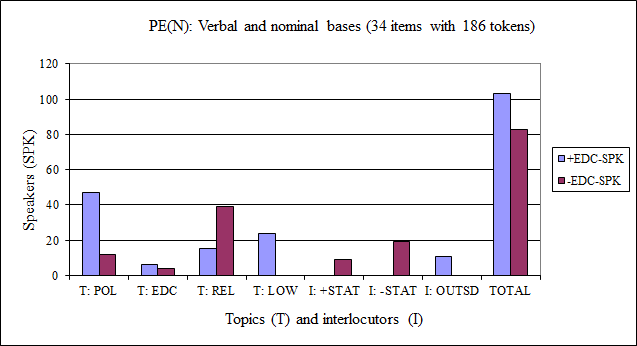
\includegraphics[scale=0.7]{./figures/Figure_3_3}
\begin{tikzpicture}
\begin{axis}[klugeaxis,title={\textscItal{pe(n)-}: Verbal and nominal bases (34 items with 186 tokens)}]
\addplot[klugedots]	coordinates {(1,47)(2,6)(3,15)(4,24)(5,0)(6,0)(7,11)(8,103)};
\addplot[klugelines] coordinates {(1,12)(2,4)(3,39)(4,0)(5,9)(6,19)(7,0)(8,83)};		
\legend{\textsc{+edc-spk},\textsc{-edc-spk}}
\end{axis}
\end{tikzpicture}
\caption[Token frequencies for {pe(n)-}prefixed lexemes with verbal and nominal bases by speakers, topics, and interlocutors]{Token frequencies for \textscItal{pe(n)-}prefixed lexemes with verbal and nominal bases by speakers, topics, and interlocutors}\label{Figure_3.3}
\end{figure}


The data given in \tabref{Table_3.13} and \figref{Figure_3.3} shows that for the 34 \textscItal{pe(n)-}prefixed lexemes, most tokens (167/186 – 90\%) can be explained in terms of speaker education levels, topics, and/or role-relations between the speakers and their interlocutors; this total includes 135/153 (88\%) tokens with verbal and 32/33 tokens (97\%) with nominal bases.


More than half of the tokens were produced by better-educated speakers (\textsc{+edc-spk}) (103/186 – 55\%), while less-educated speakers (\textsc{-edc-spk}) produced 83/186 tokens (45\%).



Two thirds of the 186 tokens (123/186 – 66\%) occurred during conversations about \textsc{high} topics, that is, political, educational or religious affairs (\textsc{pol}, \textsc{edc} and \textsc{rel}, respectively). This includes 68/103 tokens (66\%) produced by \textsc{+edc-spk} and 55/83 tokens (66\%) produced by \textsc{-edc-spk}. In addition, 11/186 tokens (6\%) occurred during conversations with an outsider, namely the author (\textsc{outsd}), all of them being \textsc{+edc-spk} tokens (11/103 – 11\%).



This leaves 52/186 tokens (28\%) that were produced when the interlocutors discussed \textsc{low} topics. This includes 24/103 \textsc{+edc-spk} tokens (23\%) and 28/83 \textsc{-edc-spk} tokens (34\%). The 28 \textsc{low} topic tokens produced by \textsc{-edc-spk} are distributed as follows. Nine tokens occurred during conversations with \textsc{+stat} Papuans (that is, 9/83 \textsc{-edc-spk} tokens – 11\%). The remaining 19 tokens (that is, 19/83 \textsc{-edc-spk} tokens – 23\%) occurred when \textsc{-edc-spk} discussed \textsc{low} topics with \textsc{-stat} Papuans, and therefore cannot be explained in terms of speaker education levels, topics, and/or role-relations. This total of 19 tokens refers to 10\% of all 186 \textscItal{pe(n)-}tokens, including 18/153 tokens (12\%) with verbal bases and 1/33 tokens (3\%) with nominal bases.\footnote{Concerning the 11 hapaxes (nine with verbal and two with nominal bases), the data suggests that seven are conditioned by the variables of speaker education levels, topics, and/or role-relations, and therefore are best explained as code-switches with \ili{Standard Indonesian}. This leaves only four hapaxes (with verbal bases) that cannot be accounted for in terms of language external factors and that are likely to result from a productive \isi{word-formation} process. For four hapaxes P=0.0376 as opposed to P=0.0591 for 11 hapaxes (N=186).}


\subsubsection[Summary and conclusions]{Summary and conclusions}\label{Para_3.1.4.5}

\largerpage
Prefix \textscItal{pe(n)-} is polyfunctional, in that it derives nouns from verbal and nominal bases. This polyfunctionality suggests that \isi{affixation} with \textscItal{pe(n)-} is a somewhat productive process (see language internal factor (\ref{List_3.1.c}) in §\ref{Para_3.1.1}, p. \pageref{List_3.1.c}).



Concerning \textscItal{pe(n)-}\isi{affixation} of verbal bases, three other observations support this conclusion: (1) the transparent form-function relationship between the derived nouns and their respective bases, (2) the large number of low frequency words and small number of high frequency words, and (3) the relative token frequencies with most bases having higher frequencies than the affixed lexemes. On the other hand, more than half of the derived lexemes were tentatively classified as SI-borrowings. These observations suggest that productivity of the \isi{affixation} process is rather limited.



As for \textscItal{pe(n)-}\isi{affixation} of nominal bases, two observations suggest that this is a productive process: (1) most of the derived lexemes are low frequency words, and (2) most bases have higher token frequencies than the affixed lexemes. On the other hand, almost all derived lexemes were tentatively classified as SI-borrowings. These findings suggest that \textscItal{pe(n)-}\isi{affixation} of nominal bases has limited productivity



As for the speech situations during which the derived nouns occurred, the vast majority of the attested tokens are conditioned by the variables of speaker education levels, topics, and/or role-relations. Hence, these items are best explained as code-switches with Indonesian.


\largerpage[2]
These findings suggest that in Papuan Malay \textscItal{pe(n)-} \isi{affixation} has, at best, margin\-al productivity.


\subsection[Prefix {\BER}- ‘\textsc{vblz}’]{Prefix \textscItal{ber-} ‘\textsc{vblz}’}\label{Para_3.1.5}

Prefix \textscItal{ber-} ‘\textsc{vblz}’ is typically attached to verbal bases, as in (\ref{Example_3.32}), or to nominal bases. Besides, the corpus also includes a few lexical items with \isi{numeral} and \isi{quantifier} bases. The prefixed lexemes have a verbal reading. As shown throughout this section, however, \isi{affixation} with \textscItal{ber-} ‘\textsc{vblz}’ is not used as a productive derivation device in Papuan Malay.

\ea
\label{Example_3.32}
\gll {\ldots} {waktu} {saya} {\bluebold{ber–buru}} {saya} {perlu} {makang} {pinang}\\ %
 { }  time  \textsc{1sg}  \textsc{vblz}–hunt  \textsc{1sg}  need  eat  betel.nut\\
\glt 
‘\ldots when I \bluebold{hunt} I need to chew betel nuts’ \textstyleExampleSource{[080919-004-NP.0011]}
\z



The corpus contains 62 derived verbs (602 tokens) prefixed with \textscItal{ber-}:\footnote{The 62 verbs include 25 hapaxes (P=0.0415); the 29 verbs with verbal bases include 11 hapaxes (P=0.0484); the 33 verbs with nominal, \isi{numeral}, or \isi{quantifier} bases include 14 hapaxes (P=0.0373).}



\begin{enumerate}
\item 
Verbs with verbal bases (29 items with 227 tokens)
\item 
Verbs with nominal, \isi{numeral}, or \isi{quantifier} bases (33 items with 375 tokens)

\end{enumerate}

The corpus also includes 16 formally complex words with non-compositional semantics, such as \textitbf{bertriak} ‘scream’, \textitbf{berjuang} ‘struggle’, or \textitbf{berlabu} ‘anchor’.



Before discussing \textscItal{ber-}\isi{affixation} of verbal bases in §\ref{Para_3.1.5.2} and of nominal, \isi{numeral}, and \isi{quantifier} bases in §\ref{Para_3.1.5.3}, the \isi{allomorphy} of \textscItal{ber-} is investigated in §\ref{Para_3.1.5.1}. Pertinent variables of the \isi{communicative event} that may impact the use of \textscItal{ber-} are explored in §\ref{Para_3.1.8}. The main findings on prefix \textscItal{ber-} are summarized and evaluated in §\ref{Para_3.1.5.4}.


\subsubsection[Allomorphy of ber-]{Allomorphy of \textscItal{ber-}}\label{Para_3.1.5.1}

Prefix \textscItal{ber-} has two allomorphs, \textitbf{ber}- and \textitbf{ba}-. The allomorphs are not governed by phonological processes.

\largerpage

\begin{table} 
\caption{Realizations of allomorph \textitbf{ber}-}\label{Table_3.14}

\begin{tabular}{lll}
\lsptoprule

 \multicolumn{1}{c}{\textitbf{ber}\textsc{-}base} & \multicolumn{1}{c}{Orthogr.} &  \multicolumn{1}{c}{Gloss}\\

\midrule
/\textstyleChCharisSIL{bɛr}–\textstyleChCharisSIL{dʒuaŋ}/ & \textitbf{berjuang} & ‘struggle (for)’\\

/\textstyleChCharisSIL{br}–\textstyleChCharisSIL{aŋkat}/ & \textitbf{brangkat} & ‘leave’\\

/\textstyleChCharisSIL{bl}–\textstyleChCharisSIL{adʒar}/ & \textitbf{blajar} & ‘study’\\

/\textstyleChCharisSIL{bɛ}–\textstyleChCharisSIL{kɛrdʒa}/ & \textitbf{bekerja} & ‘work’\\

/\textstyleChCharisSIL{bɛ}–\textstyleChCharisSIL{brapa}/ & \textitbf{bebrapa} & ‘be several’\\

\lspbottomrule
\end{tabular}
\end{table}

The form \textitbf{ber}-, in turn, has four realizations that are effected by morphologically conditioned phonological rules. More specifically, the four allomorphs are conditioned by the word-initial segment of the base word, as illustrated in \tabref{Table_3.14}: /\textstyleChCharisSIL{bɛr-}/, /\textstyleChCharisSIL{br-}/, /\textstyleChCharisSIL{bl-}/, and /\textstyleChCharisSIL{bɛ-}/. The prefix is typically realized as /\textstyleChCharisSIL{bɛr-}/. With an onset vowel, however, \textitbf{ber}- is very commonly realized as /br\textstyleChCharisSIL{-}/. When prefixed to \textitbf{ajar} ‘teach’ the prefix is realized as /\textstyleChCharisSIL{bl-}/, while it is realized as /\textstyleChCharisSIL{bɛ-}/ when affixed to \textitbf{kerja} ‘work’ or \textitbf{brapa} ‘several’.

Allomorph \textitbf{ba}- occurs much less frequently. Attested are only the 15 items listed in \tabref{Table_3.15} with a total of 37 tokens. Some of these items are alternatively realized with allomorph \textitbf{ber}-. Therefore, for each item the token frequencies for \textitbf{ba}- and for \textitbf{ber}- are given. If in a greater number of tokens the prefix is realized with /\textstyleChCharisSIL{ba-}/ rather than with /\textstyleChCharisSIL{bɛr-}/, then its orthographic representation is \textitbf{ba}- as in \textitbf{bakalay} ‘fight’. If both realizations have the same token frequencies, then the orthographic representation follows its realization in the recorded texts, as in \textitbf{bergaya} ‘put on airs’.

\begin{table}[b]
\caption{ Realizations of allomorph \textitbf{ba}-}\label{Table_3.15}


\begin{tabular}{lllrr}
\lsptoprule
 \multicolumn{1}{c}{\textitbf{ba-}base} & \multicolumn{1}{c}{Orthogr.} & \multicolumn{1}{c}{Gloss} & \multicolumn{1}{c}{\textitbf{ba-} \#} &  \multicolumn{1}{c}{\textitbf{ber-} \#}\\
\midrule

/\textstyleChCharisSIL{ba}–\textstyleChCharisSIL{kalaj}/ & \textitbf{bakalay} & ‘fight’ &  19 &  0\\

/\textstyleChCharisSIL{ba}–\textstyleChCharisSIL{taria}/ & \textitbf{bertriak}\footnote{The root is realized as /\textstyleChCharisSILviiivpt{triak}/ when speakers employ allomorph \textitbf{ber}-, whereas it is realized as /\textstyleChCharisSILviiivpt{taria}/ when speakers use allomorph \textitbf{ba}-.}
 & ‘scream’ &  3 &  18\\

/\textstyleChCharisSIL{ba}–\textstyleChCharisSIL{biŋuŋ}/ & \textitbf{babingung} & ‘be confused’ &  2 &  0\\

/\textstyleChCharisSIL{ba}–\textstyleChCharisSIL{diam}/ & \textitbf{badiam} & ‘be quiet’ &  2 &  0\\

/\textstyleChCharisSIL{ba}–\textstyleChCharisSIL{diri}/ & \textitbf{berdiri} & ‘stand’ &  1 &  54\\

/\textstyleChCharisSIL{ba}–\textstyleChCharisSIL{dara}/ & \textitbf{berdara} & ‘bloody’ &  1 &  1\\

/\textstyleChCharisSIL{ba}–duri/ & \textitbf{berduri} & ‘be thorny’ &  1 &  1\\

/\textstyleChCharisSIL{ba}–\textstyleChCharisSIL{gaja}/ & \textitbf{bergaya} & ‘put on airs’ &  1 &  1\\

/\textstyleChCharisSIL{ba}–gisi/ & \textitbf{bergisi} & ‘be nutritious’ &  1 &  1\\

/\textstyleChCharisSIL{ba}–jalang/ & \textitbf{berjalang} & ‘walk’ &  1 &  1\\

/\textstyleChCharisSIL{ba}–ribut/ & \textitbf{beribut} & ‘be noisy’ &  1 &  1\\

/\textstyleChCharisSIL{ba}–\textstyleChCharisSIL{gigit}/ & \textitbf{bagigit} & ‘bite’ &  1 &  0\\

/\textstyleChCharisSIL{ba}–\textstyleChCharisSIL{kumis}/ & \textitbf{bakumis} & ‘have a beard’ &  1 &  0\\

/\textstyleChCharisSIL{ba}–\textstyleChCharisSIL{isi}/ & \textitbf{baisi} & ‘be muscular’ &  1 &  0\\

/\textstyleChCharisSIL{ba}–\textstyleChCharisSIL{mɛkap}/ & \textitbf{bamekap} & ‘wear make-up’ &  1 &  0\\

\lspbottomrule
\end{tabular}
\end{table}

In realizing prefix \textscItal{ber-} most commonly as allomorph \textitbf{ber}- rather than as \textitbf{ba}-, Papuan Malay again contrasts with other \ili{eastern Malay varieties} such as \ili{Ambon Malay} \citep[95]{vanMinde.1997}, \ili{Banda Malay} \citep[249]{Paauw.2009}, \ili{Kupang Malay} \citep[46]{Steinhauer.1983}, \ili{Manado Malay} \citep[18]{Stoel.2005}, and North Moluccan / \ili{Ternate Malay} (\citealt[18]{Taylor.1983}; \citealt[4]{Voorhoeve.1983}; \citealt[125]{Litamahuputty.2012}). In these varieties the prefix is always realized as \textitbf{ba}-. Instead, the items prefixed with \textscItal{ber-} have more resemblance with the corresponding Indonesian items where the prefix is realized as \textitbf{ber}-. In addition, in \ili{Larantuka Malay} the prefix is also realized as \textitbf{bə}\textbf{(}\textitbf{r}\textbf{)}- {\citep[253]{Paauw.2009}}. Again this difference between Papuan Malay and the other \ili{eastern Malay varieties} points to the distinct histories of both, discussed in §\ref{Para_1.8}.


\subsubsection[Prefixed items derived from verbal bases]{Prefixed items derived from verbal bases}\label{Para_3.1.5.2}

The corpus includes 29 \textscItal{ber-}prefixed lexemes (with 227 tokens) with verbal bases, as listed in Table  \ref{Table_3.16a} and Table \ref{Table_3.16b}. Of the 29 lexemes, 11 have \isi{monovalent} bases such as stative \textitbf{diam} ‘be quiet’ or dynamic \textitbf{jalang} ‘walk’. The remaining 18 items have \isi{bivalent} bases. Of these 18 prefixed lexemes, five have monotransitive as well as intransitive uses, while 11 lexemes have intransitive uses only. These 16 lexemes have the same semantics as their \isi{bivalent} bases, as shown in (\ref{Example_3.33}) to (\ref{Example_3.43}). For the remaining two prefixed lexemes the semantics are distinct from those of their bases, as shown in (\ref{Example_3.44}) to (\ref{Example_3.50}). One of them has monotransitive as well as intransitive uses, while the other one has intransitive uses only.



Almost all of the derived lexemes are low frequency words (27 lexemes, attested with less than 20 tokens). Moreover, the token frequencies for the respective bases are (much) higher for most of the derived words (22 lexemes). This is due to the fact that the affixed lexemes and the bases have the same semantics and that, overall, speakers tend to use the bases rather than the prefixed forms, as shown in (\ref{Example_3.33}) to (\ref{Example_3.43}). Also, most of the 29 prefixed lexemes (24 items) were tentatively classified as borrowings from \ili{Standard Indonesian} (SI-borrowings) (for details see language internal factor (\ref{List_3.1.f}) in §\ref{Para_3.1.1}, p. \pageref{List_3.1.f}); in Table  \ref{Table_3.16a} and Table \ref{Table_3.16b} these items are underlined.

\begin{table}
\caption[Affixation with {ber-} of verbal bases]{Affixation with \textscItal{ber-} of verbal bases}\label{Table_3.16a}

\begin{tabularx}{\textwidth}{lllrr}
\lsptoprule

\multicolumn{1}{c}{BW} & \multicolumn{1}{c}{Item} & \multicolumn{1}{c}{Gloss} & \multicolumn{1}{c}{\textscItal{ber-} \#} &  \multicolumn{1}{c}{BW \#}\\
\midrule
\multicolumn{5}{l}{Monovalent bases: Bases and prefixed lexemes with same semantics}\\
\midrule
 \textitbf{tobat} & {\textitbfUndl{bertobat}} & ‘repent’ &  8 &  1\\

 \textitbf{beda} & {\textitbfUndl{berbeda}} & ‘be different’ &  7 &  34\\

 \textitbf{tanggung-jawap} & {\textitbfUndl{bertanggung-jawap}} & ‘be responsible’ &  5 &  6\\

 \textitbf{bahaya} & {\textitbfUndl{berbahaya}} & ‘be dangerous’ &  3 &  3\\

 \textitbf{diam} & {\textitbfUndl{badiam}} & ‘be quiet’ &  2 &  60\\

 \textitbf{bingung} & {\textitbfUndl{berbingung}} & ‘be confused’ &  2 &  30\\

 \textitbf{jalang} & {\textitbfUndl{berjalang}} & ‘walk’ &  1 &  480\\

 \textitbf{ibada} & {\textitbfUndl{beribada}} & ‘worship’ &  1 &  11\\

 \textitbf{sandar} & {\textitbfUndl{bersandar}} & ‘lean’ &  1 &  6\\

 \textitbf{hati{\Tilde}hati} & {\textitbfUndl{berhati{\Tilde}hati}} & ‘be careful’ &  1 &  5\\

 \textitbf{pisa} & {\textitbfUndl{berpisa}} & ‘be separate’ &  1 &  4\\
\midrule
\multicolumn{5}{l}{Bivalent bases: Bases and prefixed lexemes with same semantics}\\
\midrule
% \multicolumn{5}{l}{  Prefixed lexemes: Monotransitive and intransitive uses}\\

 \textitbf{buru} & {\textitbf{berburu}} & ‘hunt’ & 10 &  5\\

 \textitbf{buat} & {\textitbfUndl{berbuat}} & ‘make’ & 7 &  100\\

 \textitbf{pikir} & {\textitbfUndl{berpikir}} & ‘think’ & 8 &  102\\

 \textitbf{harap} & {\textitbfUndl{berharap}} & ‘hope’ &  1 &  8\\

 \textitbf{ribut} & {\textitbf{bribut}} & ‘trouble’ &  1 &  5\\

\tablevspace
% \multicolumn{5}{l}{  Prefixed lexemes: Monotransitive uses}\\
 \textitbf{bicara} & \textitbfUndl{berbicara} & {‘speak’} & 7 &  333\\

 \textitbf{kerja} & \textitbfUndl{bekerja} & {‘work’} & 5 &  191\\

 \textitbf{tahang} & \textitbfUndl{bertahang} & {‘hold (out/back)’} & 5 &  48\\

 \textitbf{uba} & \textitbf{bruba} & {‘change’} & 5 &  9\\

 \textitbf{gabung} & \textitbfUndl{bergabung} & {‘join’} & 4 &  3\\

 \textitbf{maing} & \textitbfUndl{bermaing} & {‘play’} &  3 &  113\\

 \textitbf{tindak} & \textitbfUndl{bertindak} & {‘act’} &  2 &  1\\

 \textitbf{ikut} & \textitbfUndl{brikut} & {‘follow’} &  1 &  259\\

 \textitbf{kumpul} & \textitbfUndl{berkumpul} & {‘gather’} &  1 &  16\\

 \textitbf{bentuk} & \textitbfUndl{berbentuk} & {‘form’} &  1 &  12\\

 \textitbf{gigit} & \textitbfUndl{bergigit} & {‘bite’} &  1 &  10\\
\lspbottomrule
\end{tabularx}
\end{table}
\begin{table}
\caption[Affixation with {ber-} of verbal bases continued]{Affixation with \textscItal{ber-} of verbal bases continued}\label{Table_3.16b}

\begin{tabularx}{\textwidth}{lllrr}
\lsptoprule

\multicolumn{1}{c}{BW} & \multicolumn{1}{c}{Item} & \multicolumn{1}{c}{Gloss} & \multicolumn{1}{c}{\textscItal{ber-} \#} &  \multicolumn{1}{c}{BW \#}\\
\midrule
\multicolumn{5}{l}{Bivalent bases: Bases and prefixed lexemes with distinct semantics}\\
\midrule
\multicolumn{5}{l}{Prefixed lexeme: Monotransitive and intransitive uses}\\

 \textitbf{ajar} (‘teach’) & {\textitbf{blajar}\hspace{2.3cm}} & ‘study’\hspace{1cm} & 51 &  41\\
\\
% \todo[inline]{check spacing}\\
\multicolumn{5}{l}{Prefixed lexeme: Monotransitive uses}\\

 \textitbf{angkat} (‘lift’) & {\textitbf{brangkat}} & ‘leave’ & 82 &  81\\

\lspbottomrule
\end{tabularx}
\end{table}

Affixation with \textscItal{ber-} of verbal bases derives lexemes that typically have the same semantics as their respective bases, with \textscItal{ber-} being glossed as ‘\textsc{vblz}’ (``verbalizer''). This applies to \textscItal{ber-}prefixed lexemes with \isi{monovalent} and with \isi{bivalent} bases.


The fact that \isi{monovalent} bases derive \textscItal{ber-}prefixed lexemes with the same semantics is illustrated with stative \textitbf{bingung} ‘be confused’ and prefixed \textitbf{berbingung} ‘be confused’ in (\ref{Example_3.33}) and (\ref{Example_3.34}), and with dynamic \textitbf{ibada} ‘worship’ and prefixed \textitbf{beribada} ‘worship’ in (\ref{Example_3.35}) and (\ref{Example_3.36}), respectively.



\begin{styleExampleTitle}
{Prefix \textscItal{ber-}: Semantics of verbal bases and derived lexemes}
\end{styleExampleTitle}

\ea
\label{Example_3.33}
\gll {memang} {sa} {punya} {ade} {sa} {juga} {\bluebold{bingung}} {dengang} {dia}\\ %
 indeed  \textsc{1sg}  \textsc{poss}  ySb  \textsc{1sg}  also  be.confused  with  \textsc{3sg}\\
\glt 
‘indeed (he was) my younger cousin, I’m also \bluebold{confused} about him’ \textstyleExampleSource{[080918-001-CvNP.0014]}
\z

 

\ea
\label{Example_3.34}
\gll {{nanti}} {di} {skola} {baru} {kamu} {\bluebold{ba–bingung}} {dengang}\\ %
 {very.soon}  at  school  and.then  \textsc{2pl}  \textsc{vblz}–be.confused  with\\

 bahasa  {Inggris}\\

 language  {English}\\

\glt 
[Addressing lazy students:] ‘later in school, then you’ll be \bluebold{confused} about English’ \textstyleExampleSource{[081115-001a-Cv.0151]}
\z

\ea
\label{Example_3.35}
\gll {orang} {jalang} {itu} {mo} {pergi} {\bluebold{ibada}}\\ %
 person  walk  \textsc{d.dist}  want  go  worship\\
\glt 
[About a youth retreat:] ‘people doing that traveling want to go (and) \bluebold{worship}’ \textstyleExampleSource{[081006-016-Cv.0017]}
\z

\ea
\label{Example_3.36}
\gll {{nanti}} {{kita}} {\bluebold{ber–ibada}} {selesay} {malam} {ka}\\ %
 {very.soon}  {\textsc{1pl}}  \textsc{vblz}–worship  finish  night  maybe\\
\gll baru  {sa}  {pergi}\\
 and.then  {\textsc{1sg}}  {go}\\
\glt 
‘later, after we have \bluebold{worshipped}, maybe in the evening, and then I’ll go (there)’ \textstyleExampleSource{[080918-001-CvNP.0016]}\footnotetext{The original recording says \textitbf{kita i beribada selesay}. Most likely the speaker wanted to say \textitbf{kita ibada selesay} ‘after we have worshipped’ but cut himself off to replace \textitbf{ibada} ‘worship’ with \textitbf{beribada} ‘worship’.}
\z

Bivalent bases also derive \textscItal{ber-}prefixed lexemes that have the same semantics as their bases, as shown in (\ref{Example_3.37}) to (\ref{Example_3.43}). As discussed in §\ref{Para_11.1.2}, \isi{bivalent} verbs have not only monotransitive but also intransitive uses. The same applies to some of the \textscItal{ber-}prefixed lexemes, as illustrated in (\ref{Example_3.37}) to (\ref{Example_3.40}).



\begin{styleExampleTitle}
{Prefix \textscItal{ber-}: Same semantics of verbal bases and derived lexemes}
\end{styleExampleTitle}

\ea
\label{Example_3.37}
\gll {jadi} {kitorang} {bingung} {\bluebold{pikir}} {itu} {pen–jaga} {kubur\bluebold{–}ang}\\ %
 so  \textsc{1pl}  be.confused  think  \textsc{d.dist}  \textsc{ag}–guard  bury–\textsc{pat}\\
\glt 
‘so we’re confused to \bluebold{think (about)}, what’s-its-name, a guard (for) the grave’ \textstyleExampleSource{[080923-007-Cv.0024]}
\z

\ea
\label{Example_3.38}
\gll   {\ldots}  tapi  ana{\Tilde}ana  ni  dong  tida  taw  \bluebold{ber–pikir}  itu\\
  { }  but  \textsc{rdp}{\Tilde}child  \textsc{d.prox}  \textsc{3pl}  \textsc{neg}  know  \textsc{vblz}–think  \textsc{d.dist}\\
\glt 
[About impolite teenagers:] ‘{\ldots} but these kids they don’t know (how) to \bluebold{think (about)} those (feelings of mine)’ \textstyleExampleSource{[081115-001b-Cv.0037]}
\z

\ea
\label{Example_3.39}
\gll {skarang}  orang  su  tra  \bluebold{pikir}  tentang\\
 {now}  person  already  \textsc{neg}  think  about\\
\gll hal  {ke–benar–ang}\\
 thing  {\textsc{nmlz}–be.true–\textsc{nmlz}}\\
\glt 
‘nowadays, the people already don’t \bluebold{think} about things (related to) truth’ \textstyleExampleSource{[081006-032-Cv.0016]}
\z

\ea
\label{Example_3.40}
\gll {\ldots} {karna} {dia} {\bluebold{ber–pikir}} {tentang} {dia} {punya} {badang}\\ %
 { }  because  \textsc{3sg}  \textsc{vblz}–think  about  \textsc{3sg}  \textsc{poss}  body\\
\glt 
‘[she doesn’t think about serving my or her guests] because she \bluebold{thinks} about her body’ \textstyleExampleSource{[081006-032-Cv.0062]}
\z


Most \textscItal{ber-}prefixed lexemes with \isi{bivalent} bases, however, have intransitive uses only, while their bases can be used mono- or intransitively. This is illustrated with \textitbf{bicara} ‘speak’ and \textitbf{berbicara} ‘speak’ in (\ref{Example_3.41}) to (\ref{Example_3.43}).



\begin{styleExampleTitle}
Prefix \textscItal{ber-}: Semantics and distribution of verbal bases and derived lexemes
\end{styleExampleTitle}

\ea
\label{Example_3.41}
\gll {baru} {de} {\bluebold{bicara}} {sa} {deng} {bahasa} {Inggris}\\ %
 and.then  \textsc{3sg}  speak  \textsc{1sg}  with  language  English\\

\glt 
‘and then she \bluebold{talked (to)} me in English’ \textstyleExampleSource{[081115-001a-Cv.0229]}
\z

\ea
\label{Example_3.42}
\gll  de  \bluebold{bicara}  trus\\
 \textsc{3sg}  speak  be.continuous\\
\glt 
‘he kept \bluebold{talking}’ \textstyleExampleSource{[080922-010a-CvNF.0145]}
\z
\ea
\label{Example_3.43}
\gll {baru} {nanti} {\bluebold{ber–bicara}} {untuk} {nika}\\ %
 and.then  very.soon  \textsc{vblz}–speak  for  marry.officially\\
\glt 
[About wedding customs:] ‘and then very soon (they’ll) \bluebold{talk} about marrying’ \textstyleExampleSource{[081110-006-CvEx.0050]}
\z


The corpus includes only two \textscItal{ber-}prefixed lexemes that have distinct semantics vis-à-vis their \isi{bivalent} bases, namely \textitbf{ajar} ‘teach’ and prefixed \textitbf{blajar} ‘study’, and \textitbf{angkat} ‘lift’ and prefixed \textitbf{brangkat} ‘leave’ as shown in (\ref{Example_3.44}) to (\ref{Example_3.50}). Both \textitbf{ajar} ‘teach’ and \textitbf{blajar} ‘study’ are used monotransitively as in (\ref{Example_3.44}) and (\ref{Example_3.45}), as well as intransitively as in (\ref{Example_3.46}) and (\ref{Example_3.47}), respectively; in each case both lexemes maintain their distinct semantics.



\begin{styleExampleTitle}
{Prefix \textscItal{ber-}: Distinct semantics and same distribution of verbal bases and derived lexemes}
\end{styleExampleTitle}

\ea
\label{Example_3.44}
\gll {de} {\bluebold{ajar}} {dorang} {tu} {untuk} {baik}\\ %
 \textsc{3sg}  teach  \textsc{3pl}  \textsc{d.dist}  for  be.good\\
\glt 
‘she \bluebold{teaches} them there for (their own) good’ \textstyleExampleSource{[081115-001a-Cv.0216]}
\z

\ea
\label{Example_3.45}
\gll {Ise} {de} {\ldots} {{ikut}} {bahasa} {Inggris} {\bluebold{bl–ajar}} {kursus,}\\ %
 Ise  \textsc{3sg} {}   {follow}  language  English  \textsc{vblz}–teach  course\\
\gll {bahasa}  {Inggris}  {dulu}\\
 {language}  {English}  {first}\\
\glt 
‘Ise will participate in an English (course), (she’ll) \bluebold{study} a course, an English language course first’ \textstyleExampleSource{[081025-003-Cv.0223]}
\z

\ea
\label{Example_3.46}
\gll {de} {suda} {\bluebold{ajar}} {bagus} {tiap} {sore} {itu}\\ %
 \textsc{3sg}  already  teach  be.good  every  afternoon  \textsc{d.dist}\\
\glt 
‘she’s already been \bluebold{teaching} well, each and every afternoon’ \textstyleExampleSource{[081115-001a-Cv.0126]}
\z
\ea
\label{Example_3.47}
\gll {dong} {tida} {\bluebold{bl–ajar}} {baik}\\ %
 \textsc{3pl}  \textsc{neg}  \textsc{vblz}–teach  be.good\\

\glt 
‘they don’t \bluebold{study} well’ \textstyleExampleSource{[081115-001b-Cv.0067]}
\z


Bivalent \textitbf{angkat} ‘lift’ and prefixed \textitbf{brangkat} ‘leave’ also have distinct semantics. In addition, they also have a distinct distribution. The base \textitbf{angkat} ‘lift’ is used monotransitively, as well as intransitively, as in (\ref{Example_3.48}) and (\ref{Example_3.49}), respectively. By contrast, \textitbf{brangkat} ‘leave’ is always used intransitively, as in (\ref{Example_3.50}).



\begin{styleExampleTitle}
{Prefix \textscItal{ber-}: Distinct semantics and distinct distribution of \isi{verbal base} and derived lexeme}
\end{styleExampleTitle}
\ea
\label{Example_3.48}
\gll {bapa} {de} {\bluebold{angkat}} {rotang} {besar}\\ %
 father  \textsc{3sg}  lift  rattan  be.big\\
\glt 
‘father \bluebold{picked up} a big rattan (stick)’ \textstyleExampleSource{[080921-004a-CvNP.0084]}
\z
\ea
\label{Example_3.49}
\gll {sa} {sendiri} {tra} {bisa} {\bluebold{angkat}}\\ %
 \textsc{1sg}  be.alone  \textsc{neg}  be.able  lift\\
\glt 
‘[the pig was very big,] I alone could not \bluebold{transport} (it)’ \textstyleExampleSource{[080919-003-NP.0008]}
\z
\ea
\label{Example_3.50}
\gll {skarang} {de} {mo} {\bluebold{br–angkat}}\\ %
 now  \textsc{3sg}  want  \textsc{vblz}–lift\\
\glt 
‘then he wanted to \bluebold{leave}’ \textstyleExampleSource{[080919-007-CvNP.0023]}
\z


In summary, with the exception of the last two lexemes, \textscItal{ber-}prefixed verbs have the same semantics as their respective bases. This suggests that in Papuan Malay \isi{affixation} of verbal bases with prefix \textscItal{ber-} is not a productive process. Instead, the attested prefixed lexemes and their bases are taken as pairs of words from two different speech varieties: the unaffixed items are native Papuan Malay lexemes whereas the corresponding affixed items are SI-borrowings.



Given these properties, Papuan Malay \textscItal{ber-} contrasts with the corresponding prefix in other Malay varieties. In most \ili{eastern Malay varieties}, the corresponding prefix \textitbf{ba}- forms verbs with a variety of meanings. The most common ones are durative and reflexive meanings, which are reported for \ili{Ambon Malay} \citep[96–98]{vanMinde.1997}, \ili{Banda Malay} \citep[249--250]{Paauw.2009},\footnote{For \ili{Banda Malay}, \citet[249]{Paauw.2009} reports that \textitbf{ba}- does not form verbs with reflexive meanings.} \ili{Manado Malay} \citep[18–22]{Stoel.2005}, and North Moluccan / \ili{Ternate Malay} (\citealt[18]{Taylor.1983}; \citealt[125–127]{Litamahuputty.2012}). In \ili{Kupang Malay} \citep[46–49]{Steinhauer.1983} and \ili{Larantuka Malay} \citep[249–254-255]{Paauw.2009}, the prefix typically signals durative and reciprocal meanings. In \ili{Standard Indonesian}, the main function of the corresponding prefix \textitbf{ber-} is to create \isi{monovalent} verbs (\citealt[131]{Englebretson.2003}; \citeyear*[96]{Englebretson.2007}). When attached to verbal bases, the prefix indicates “that the subject of the utterance is the patient, that is, the experiencer of the action” \citep[134–138]{Mintz.1994}.


\subsubsection[Prefixed items derived from nominal, {numeral}, or {quantifier} bases]{Prefixed items derived from nominal, {numeral}, or {quantifier} bases}\label{Para_3.1.5.3}

The corpus contains 33 \textscItal{ber-}prefixed lexemes (with 375 tokens), as listed in  \tabref{Table_3.17a} and \tabref{Table_3.17b}: 30 lexemes with nominal bases (362 tokens), two lexemes with \isi{numeral} bases (7 tokens), and one lexeme with a \isi{quantifier} base (6 tokens).



Most of the derived lexemes are low frequency words (29 lexemes, attested with less than 20 tokens). Besides, the token frequencies for the respective bases are (much) higher for most of the derived words (21 lexemes). This is due to the fact that Papuan Malay speakers typically use alternative analytical constructions to convey the meanings of the prefixed lexemes, as shown below in (\ref{Example_3.51}) to (\ref{Example_3.56}). Further, most of the 33 items (25 items) were tentatively classified as SI-borrowings (for details see language internal factor (\ref{List_3.1.f}) in §\ref{Para_3.1.1}, p. \pageref{List_3.1.f}); in \tabref{Table_3.17a} and \tabref{Table_3.17b} these items are underlined.

\begin{table}[b]
\caption[Affixation with {ber-} of nominal, \isi{numeral}, and \isi{quantifier} bases]{Affixation with \textscItal{ber-} of nominal, \isi{numeral}, and \isi{quantifier} bases}\label{Table_3.17a}
\begin{tabularx}{\textwidth}{llll>{\raggedleft}Xr}
\lsptoprule
 \multicolumn{1}{c}{BW} & \multicolumn{1}{c}{Gloss} & \multicolumn{1}{c}{Item} & \multicolumn{1}{c}{Gloss} & \multicolumn{1}{c}{\textscItal{ber-} \#} &  \multicolumn{1}{c}{BW \#}\\
\midrule
\multicolumn{6}{l}{Nominal bases}\\
\midrule
\textitbf{doa} & ‘prayer’ & \textitbf{berdoa} & ‘pray’ &  136 &  20\\

\textitbf{arti} & ‘meaning’ & \textitbf{brarti} & ‘mean’ &  89 &  7\\

\textitbf{diri} & ‘self’ & \textitbf{berdiri} & ‘stand’ &  55 &  14\\

\textitbf{usaha} & ‘effort’ & \textitbf{berusaha} & ‘attempt’ &  25 &  2\\

\textitbf{dosa} & ‘sin’ & \textitbf{berdosa} & ‘sin’ &  6 &  4\\

\textitbf{saksi} & ‘witness’ & \textitbfUndl{bersaksi} & ‘testify’ &  6 &  2\\

\textitbf{hasil} & ‘result’ & \textitbf{berhasil} & ‘succeed’ &  6 &  13\\

\textitbf{kwasa} & ‘power’ & \textitbfUndl{berkwasa} & ‘be powerful’ &  4 &  25\\

\textitbf{hak} & ‘right’ & \textitbfUndl{berhak} & ‘have right’ &  4 &  15\\

\textitbf{sodara} & ‘sibling’ & \textitbfUndl{bersodara} & ‘be siblings’ &  3 &  127\\

\textitbf{kebung} & ‘garden’ & \textitbfUndl{berkebung} & ‘do farming’ &  3 &  61\\

\textitbf{ade-kaka} & ‘siblings’ & \textitbfUndl{brade-kaka} & ‘be siblings’ &  2 &  26\\

\textitbf{malam} & ‘night’ & \textitbfUndl{bermalam} & ‘overnight’ &  2 &  191\\

\textitbf{bahasa} & ‘language’ & \textitbfUndl{berbahasa} & ‘speak’ &  2 &  136\\

\textitbf{temang} & ‘friend’ & \textitbfUndl{bertemang} & ‘be friends’ &  2 &  85\\

\textitbf{kluarga} & ‘family’ & \textitbfUndl{berkluarga} & ‘have family’ &  2 &  49\\

\textitbf{gaya} & ‘manner’ & \textitbf{bergaya} & ‘put on airs’ &  2 &  7\\

\textitbf{ana} & ‘child’ & \textitbf{brana} & ‘give birth’ &  1 &  739\\

\textitbf{bua} & ‘fruit’ & \textitbfUndl{berbua} & ‘have fruit’ &  1 &  38\\

\textitbf{dara} & ‘blood’ & \textitbfUndl{berdara} & ‘bleed’ &  1 &  27\\

\textitbf{sifat} & ‘characteristic’ & \textitbfUndl{bersifat} & ‘have characteristics of’ &  1 &  18\\

\textitbf{duri} & ‘thorn’ & \textitbfUndl{berduri} & ‘have thorns’ &  1 &  8\\

\textitbf{harga} & ‘value’ & \textitbfUndl{berharga} & ‘be valuable’ &  1 &  4\\

\textitbf{syukur} & ‘thanks’ & \textitbfUndl{bersyukur} & ‘give thanks’ &  1 &  2\\

\textitbf{fungsi} & ‘function’ & \textitbfUndl{berfungsi} & ‘function’ &  1 &  1\\

\textitbf{gisi} & ‘nutrient’ & \textitbfUndl{bergisi} & ‘be nutritious’ &  1 &  1\\

\textitbf{isi} & ‘content’ & \textitbfUndl{baisi} & ‘be muscular’ &  1 &  1\\
\lspbottomrule
\end{tabularx}
\end{table}
\begin{table}

\caption[Affixation with {ber-} of nominal, \isi{numeral}, and \isi{quantifier} bases continued]{Affixation with \textscItal{ber-} of nominal, \isi{numeral}, and \isi{quantifier} bases continued}\label{Table_3.17b}
{\setlength{\tabcolsep}{3pt}
\begin{tabularx}{\textwidth}{llllrr}
\lsptoprule

 BW & Gloss & Item & Gloss & \textscItal{ber-} \#\hspace{2mm} &  BW \#\\
\midrule

\textitbf{komunikasi} & ‘communica\-tion’ & \textitbfUndl{berkomuni\-}\textitbfUndl{kasi} & ‘communicate’ &  1 &  1\\

\textitbf{kumis} & ‘beard’ & \textitbfUndl{bakumis} & ‘have a beard’ &  1 &  1\\

\textitbf{mekap} & ‘make-up’ & \textitbfUndl{bamekap} & ‘wear make-up’ &  1 &  1\\
\midrule
\multicolumn{6}{l}{Numeral bases}\\
\midrule
\textitbf{satu} & ‘one’ & \textitbfUndl{bersatu} & ‘be one’ &  6 &  516\\

\textitbf{empat} & ‘four’ & \textitbfUndl{berempat} & ‘be four’ &  1 &  66\\
\midrule
\multicolumn{6}{l}{Quantifier base}\\
\midrule
\textitbf{brapa} & ‘several’ & \textitbfUndl{bebrapa} & ‘be several’ &  6 &  109\\

\lspbottomrule
\end{tabularx}
}
\end{table}

\newpage 
Affixation with \textscItal{ber-} derives \isi{monovalent} verbs with the general meaning of ‘be/have/ do \textsc{base}’. Examples are \textitbf{brarti} ‘have the meaning of’ or ‘mean’, \textitbf{berdoa} ‘do prayer’ or ‘pray’, \textitbf{bersatu} ‘be one’, or \textitbf{bebrapa} ‘be several’. The \isi{monovalent} \isi{verb} \textitbf{berdiri} ‘stand’ is an exception. Historically related to the \isi{noun} \textitbf{diri} ‘self’, it does not have a transparent form-function relationship to its base. The transparent form-function relationship between the remaining 32 items and their bases suggests that these lexemes are the result of a productive \isi{affixation} process. Two observations are made, however.


First, the data indicates that Papuan Malay speakers prefer to employ analytical constructions to express the meanings conveyed by the prefixed items, as illustrated in (\ref{Example_3.51}) to (\ref{Example_3.56}). To communicate ‘have \textsc{base}’, speakers typically use the existential \isi{verb} \textitbf{ada} ‘exist’ rather than the prefixed form, as shown in (\ref{Example_3.51}) with \textitbf{ada duri} versus \textitbf{berduri} ‘have thorns’.

\ea
\label{Example_3.51}
\gll {{ada}} {{\ldots}} {dua} {{macang}} {{jenis}} {{ada}} {{yang}} {{\bluebold{ber}\bluebold{–}\bluebold{duri}}} {ada} {yang}\\ %
 {exist}  {}  two  {variety}  {kind}  {exist}  {\textsc{rel}}  {\textsc{vblz}–thorn}  exist  \textsc{rel}\\
\\
\gll tida  {\ldots}  {kang}  {ada}  {sagu}  {yang}  {tida}  \bluebold{ada}  {\bluebold{duri}}\\
 \textsc{neg}  {}  {you.know}  {exist}  {sago}  {\textsc{rel}}  {\textsc{neg}}  exist  {thorn}\\

\glt 
‘there are {\ldots} two kinds (of sago palms), ones that \bluebold{have thorns} and ones that don’t (have thorns) {\ldots} you know (there are) sago (palms) that don’t \bluebold{have thorns}’ \textstyleExampleSource{[081014-006-CvPr.0007/0009]}
\z


To express ‘be \textsc{base}’, speakers use a nominal predicate such as \textitbf{ade-kaka} ‘siblings’ in (\ref{Example_3.52}), rather than the respective prefixed form \textitbf{brade-kaka} ‘be siblings’ as in (\ref{Example_3.53}).

\ea
\label{Example_3.52}
\glll {jadi} {saya} {dengang} {dia} \bluebold{ade-kaka} {sunggu}\\ %
 {} {} {} {} {ySb-oSb}\\
 so  \textsc{1sg}  with  \textsc{3sg}  siblings  be.true\\
\glt 
‘so I and she \bluebold{are} full \bluebold{siblings}’ \textstyleExampleSource{[080927-009-CvNP.0044]}
\z

\ea
\label{Example_3.53}
\gll {jadi} {saya} {dengang} {kaka} {Nofita} {masi} {\bluebold{br}\bluebold{–}\bluebold{ade-kaka}}\\ %
 so  \textsc{1sg}  with  oSb  Nofita  still  \textsc{vblz}–siblings\\
\glt 
‘so I and older sister Nofita \bluebold{are} still \bluebold{siblings}’ \textstyleExampleSource{[080927-007-CvNP.0022]}
\z


To communicate ‘do \textsc{base}’, speakers typically employ alternative verbs. They tend to say, for example, \textitbf{biking kebung} ‘make/work a garden’ as in (\ref{Example_3.54}), rather than use prefixed \textitbf{berkebung} ‘do farming’ as in (\ref{Example_3.55}). Likewise, it is more common to say \textitbf{taw bahasa X} ‘speak language X’ than to use prefixed \textitbf{berbahasa X} ‘speak language X’ as in (\ref{Example_3.56}).

\ea
\label{Example_3.54}
\gll {kalo} {di} {Arbais} {prempuang} {bisa} {\bluebold{biking}} {\bluebold{kebung}}\\ %
 if  at  Arbais  woman  be.able  make  garden\\
\glt 
‘as for Arbais, (there) the women can \bluebold{work a garden}’ \textstyleExampleSource{[081014-007-CvEx.0035]}\\
\z

\ea
\label{Example_3.55}
\gll {bapa} {pergi} {\bluebold{ber}\bluebold{–}\bluebold{kebung}} {saya} {ikut}\\ %
 father  go  \textsc{vblz}–garden  \textsc{1sg}  follow\\
\glt 
‘(whenever my) father went to \bluebold{do farming} I went with (him)’ \textstyleExampleSource{[081110-008-CvNP.0002]}\\
\z

\ea
\label{Example_3.56}
\gll {jadi} {{tong}} {cuma} {{\bluebold{taw}}} {{\bluebold{bahasa}}} {\bluebold{Yali}} {{\ldots}} {{tapi}} {sa} {{bilang}}\\ %
 so  {\textsc{1pl}}  just  {know}  {language}  Yali  {}  {but}  \textsc{1sg}  {say}\\
\gll {kamu}  {ber\bluebold{–}syukur}  {karna}  {bisa}  {\ldots}  {\bluebold{ber}\bluebold{–}\bluebold{bahasa}}  \bluebold{Yali}\\
 {\textsc{2pl}}  {\textsc{vblz}\bluebold{–}thank.God}  {because}  {be.able}  {}  {\textsc{vblz}–language}  Yali\\
\glt 
`so we only \bluebold{spoke Yali} {\ldots} but I said, ``you (should) be grateful because (you) can \bluebold{speak Yali}''' \textstyleExampleSource{[081011-022-Cv.0101/0184]}
\z


Second, the exchange in (\ref{Example_3.57}) suggests that the high frequency items listed in \tabref{Table_3.17a} and \tabref{Table_3.17b} may well have non-compositional semantics for Papuan Malay speakers. In a conversation about religious affairs, the speaker produced \textitbf{diberdoa} ‘be prayed for’. This item is ungrammatical in both Papuan Malay and \ili{Standard Indonesian}. Papuan Malay does not have a morphologically marked undergoer voice. The \ili{Standard Indonesian} undergoer voice marker \textitbf{di}- cannot co-occur with prefix \textitbf{ber}-, but always replaces it. This example suggests that the speaker perceives \textitbf{berdoa} ‘pray’ as a monomorphemic word to which she affixed the Indonesian undergoer voice marker \textitbf{di}- in an attempt to approximate Indonesian.


\ea
\label{Example_3.57}
\gll {bebang} {masala} {de} {punya} {dia} {perlu} {\ldots} {harus} {\bluebold{di}\bluebold{–}\bluebold{ber}\bluebold{–}\bluebold{doa}}\\ %
 burden  problem  \textsc{3sg}  \textsc{poss}  \textsc{3sg}  need {}   have.to  \textsc{uv}–\textsc{vblz}–prayer\\
\glt [Conversation about problems of a church congregation:] ‘(all) burdens (and) problems (that) it has, (the congregation) needs {\ldots} has to \bluebold{be prayed for}’ \textstyleExampleSource{[080917-008-NP.0089/0091]}
\z

\subsubsection[Summary and conclusions]{Summary and conclusions}\label{Para_3.1.5.4}

Prefix \textscItal{ber-} is a polyfunctional affix that derives lexemes from verbal, nominal, \isi{numeral}, and \isi{quantifier} bases. This polyfunctionality suggests that in Papuan Malay \isi{affixation} with \textscItal{ber-} is a somewhat productive process (see language internal factor (\ref{List_3.1.c}) in §\ref{Para_3.1.1}, p. \pageref{List_3.1.c}). Two other observations support this conclusion: (1) the large number of low frequency words and small number of high frequency words, and (2) the relative token frequencies with most bases having higher frequencies than the affixed lexemes.



Four other observations, however, do not support the conclusion that \isi{affixation} with \textscItal{ber-} is a productive process: (1) for the prefixed lexemes with verbal bases, the derived lexemes have the same semantics as their bases, (2) for lexemes with nominal bases, speakers prefer to use alternative analytical constructions rather than the affixed lexemes, (3) high frequency items may well have non-compositional semantics for Papuan Malay speakers, and (4) most of the lexemes with verbal or nominal bases were tentatively classified as SI-borrowings.



Taken together, these findings indicate that Papuan Malay speakers do not employ prefix \textscItal{ber-} as a productive device to derive new words. This conclusion is also supported by the findings of a domain analysis which indicate that most of the attested tokens can be accounted for in terms of the variables of speaker education levels, topics, and/or role-relations (details are discussed in §\ref{Para_3.1.8}, together with the findings for suffix \textitbf{-nya} ‘\textsc{3possr}’ and circumfix \textitbf{ke}\textitbf{-}/\textitbf{-}\textitbf{ang} ‘\textsc{nmlz}’). Therefore, these lexemes are best explained as code-switches with Indonesian. (For a detailed discussion of prefix \textitbf{ber}- in \ili{Standard Indonesian} and Standard Malay see \citealt{Adelaar.1992}; \citealt{Mintz.1994}; \citealt{Sneddon.2010}.)


The conclusion that in Papuan Malay prefix \textscItal{ber-} is unproductive again sets Papuan Malay apart from other \ili{eastern Malay varieties}. In regional varieties such as \ili{Ambon Malay} \citep[96–98]{vanMinde.1997}, \ili{Banda Malay} \citep[249–250]{Paauw.2009}, \ili{Larantuka Malay} \citep[253–255]{Paauw.2009}, \ili{Manado Malay} \citep[18–22]{Stoel.2005}, and North Moluccan / \ili{Ternate Malay} (\citealt[18]{Taylor.1983}; \citealt[125--127]{Litamahuputty.2012}) the prefix is a productive derivational device.\footnote{{\citet[4]{Voorhoeve.1983}} considers prefix \textitbf{ba}- to be unproductive.} This distinction between Papuan Malay and the other \ili{eastern Malay varieties} once again hints at the separate histories of both, discussed in §\ref{Para_1.8}.


\subsection{Suffix \textitbf{-nya} ‘\textsc{3possr}’}\label{Para_3.1.6}

Suffix \textitbf{-nya} ‘\textsc{3possr}’ is typically attached to nominal bases to indicate possessive relations, as illustrated in (\ref{Example_3.58}). In addition, a considerable number of suffixed lexemes have verbal bases, while a small number of lexemes have prepositional, adverbial, \isi{locative}, or \isi{demonstrative} bases. However, \isi{affixation} with \textitbf{-nya} ‘\textsc{3possr}’ is not used as a productive derivation device in Papuan Malay.


\ea
\label{Example_3.58}
\gll {jadi} {\bluebold{ana–nya}} {hidup,} {ana} {itu} {masi} {ada}\\ %
 so  child–\textsc{3possr}  live  child  \textsc{d.dist}  still  exist\\
\glt 
‘so \bluebold{her child} lives, that child still exists’ \textstyleExampleSource{[080921-005-CvNP.0007]}
\z



The corpus contains 123 lexical items (387 tokens) suffixed with \textitbf{-nya}:\footnote{The 123 suffixed lexemes include 68 hapaxes (P=0.1757); the 81 lexemes with nominal bases include 44 hapaxes (P=0.1549); the 36 lexemes with verbal bases include 21 hapaxes (P=0.2561); the five lexemes with other bases include three hapaxes (P=0.1500).}



\begin{enumerate}
\item 
Suffixed items with nominal bases (82 items with 285 tokens)
\item 
Suffixed items with verbal bases (36 items with 82 tokens)
\item 
Suffixed items with other bases (five items with 20 tokens)

\end{enumerate}

The corpus also contains seven formally complex words with non-composi\-tion\-al semantics. All seven items have adverbial function, such as \textitbf{misalnya} ‘for example’ or \textitbf{akirnya} ‘finally’.



Suffixed lexemes with nominal bases are discussed in §\ref{Para_3.1.6.1}, those with verbal bases in §\ref{Para_3.1.6.2}, and those with other bases in §\ref{Para_3.1.6.3}. Pertinent variables of the \isi{communicative event} that may impact the use of \textitbf{-nya} are explored in §\ref{Para_3.1.8}. The main findings on suffix \textitbf{-nya} are summarized and evaluated in §\ref{Para_3.1.6.4}.


\subsubsection[Suffixed items derived from nominal bases]{Suffixed items derived from nominal bases}\label{Para_3.1.6.1}

The corpus contains 82 \textitbf{-nya}{}-suffixed lexemes (with 285 tokens) with nominal bases, where \textitbf{-nya} typically signals possession. As an extension of the possessive-marking function, some of the derived items listed in \tabref{Table_3.18} function as sentence adverbs, namely \textitbf{maksutnya} ‘that is to say’ (literally ‘the purpose of’), \textitbf{katanya} ‘it is being said’ (literally ‘the word of’), and \textitbf{artinya} ‘that means’ (literally ‘the meaning of’).



Derived words with token frequencies of five or more are listed in \tabref{Table_3.18}. All but two of the derived lexemes are low frequency words (80 items, attested with less than 20 tokens). Besides, the token frequencies for the respective bases are (much) higher for most of the derived words (65 lexemes). Of the 82 suffixed lexemes, 76 were tentatively classified as borrowings from \ili{Standard Indonesian} (SI-borrowings) (for details see language internal factor (\ref{List_3.1.f}) in §\ref{Para_3.1.1}, p. \pageref{List_3.1.f}); in \tabref{Table_3.18} these items are underlined. The exceptions are the three derived lexemes that function as sentence adverbs, two of which are presented in context in (\ref{Example_3.61}) and (\ref{Example_3.62}).



The low token frequencies for the derived lexemes result from the fact that Papuan Malay speakers usually use an alternative strategy to express possessive relations. Instead of suffixing \textitbf{-nya} to a \isi{nominal base}, Papuan Malay encodes \isi{adnominal possession} by an analytical construction with \textitbf{punya}, or reduced \textitbf{pu}, ‘\textsc{poss}’ (see \chapref{Para_9}). The ``\textitbf{punya} \#'' column in \tabref{Table_3.18} lists the token frequencies for adnominal possessive constructions with \textitbf{punya}/\textitbf{pu} ‘\textsc{poss}’. Examples are given in (\ref{Example_3.59}) and (\ref{Example_3.60}).

\begin{table}
\caption{Affixation with \textitbf{-nya} of nominal bases}\label{Table_3.18}
\begin{tabular}{llllrr}
\lsptoprule

 BW & Gloss & Item & \multicolumn{1}{c}{Gloss} & \textitbf{-nya} \# &  \textitbf{punya} \#\\
\midrule
\textitbf{nama} & ‘name’ & \textitbfUndl{namanya} & ‘the name of’ &  23 &  38\\

\textitbf{istri} & ‘wife’ & \textitbfUndl{istrinya} & ‘the wife of’ &  11 &  22\\

\textitbf{ana} & ‘child’ & \textitbfUndl{ananya} & ‘the child of’ &  7 &  119\\

\textitbf{orang} & ‘person’ & \textitbfUndl{orangnya} & ‘the person of’ &  6 &  8\\

\textitbf{ruma} & ‘house’ & \textitbfUndl{rumanya} & ‘the house of’ &  5 &  43\\

\textitbf{hasil} & ‘product’ & \textitbfUndl{hasilnya} & ‘the product of’ &  5 &  2\\

\textitbf{istila} & ‘term’ & \textitbfUndl{istilanya} & ‘the term of/for’ &  5 &  1\\

\textitbf{dalam} & ‘inside’ & \textitbfUndl{dalamnya} & ‘the inside of’ &  5 &  {}-{}-{}-\\

\textitbf{maksut} & ‘purpose’ & \textitbf{maksutnya} & ‘that is to say’ &  70 &  3\\

\textitbf{kata} & ‘word’ & \textitbf{katanya} & ‘it is being said’ &  19 &  {}-{}-{}-\\

\textitbf{arti} & ‘meaning’ & \textitbf{artinya} & ‘that means’ &  17 &  {}-{}-{}-\\

\lspbottomrule
\end{tabular}
\end{table}

In (\ref{Example_3.59}), \textitbf{-nya} is suffixed to the \isi{nominal base} \textitbf{nama} ‘name’, giving the possessive reading \textitbf{namanya} ‘her name’. By contrast, (\ref{Example_3.60}) shows the inherited analytical strategy of expressing the same meaning with possessive marker \textitbf{pu} ‘\textsc{poss}’.



\begin{styleExampleTitle}
{Suffix \textitbf{-nya}: Possessive reading of derived lexemes}
\end{styleExampleTitle}
\ea
\label{Example_3.59}
\gll {\bluebold{nama–nya}} {Madga}\\ %
 name–\textsc{3possr}  Madga\\
\glt 
‘\bluebold{her name} is Madga’ \textstyleExampleSource{[081011-005-Cv.0027]}
\z

\ea
\label{Example_3.60}
\gll {\bluebold{de}} {\bluebold{pu}} {\bluebold{nama}} {Martin}\\ %
 \textsc{3sg}  \textsc{poss}  name  Martin\\
\glt 
‘\bluebold{his name} is Martin’ \textstyleExampleSource{[081011-022-Cv.0241]}
\z


The examples in (\ref{Example_3.61}) and (\ref{Example_3.62}) illustrate the uses of \textitbf{maksutnya} ‘that is to say’ and \textitbf{katanya} ‘it is being said’, respectively, as sentence adverbs.



\begin{styleExampleTitle}
Suffix \textitbf{-nya}: Adverbial reading of derived lexemes
\end{styleExampleTitle}

\ea
\label{Example_3.61}
\gll {\ldots} {\bluebold{maksut–nya}} {saya} {harus} {dayung} {dulu} {dengang} {prahu}\\ %
  {}   purpose–\textsc{3possr}  \textsc{1sg}  have.to  row  first  with  boat\\
\glt 
‘[I’m getting ready, I take my bow and arrows and an oar,] \bluebold{that is to say}, I have to row first with a boat’ \textstyleExampleSource{[080919-004-NP.0008]}
\z

\ea
\label{Example_3.62}
\gll {\bluebold{kata–nya}} {orang} {Sulawesi} {smua}\\ %
 word–\textsc{3possr}  person  Sulawesi  all\\

\glt
‘\bluebold{it’s being said} (that) they are all Sulawesi people’ (Lit. ‘(the) Sulawesi people (are) all’) \textstyleExampleSource{[081029-005-Cv.0106]}
\z

\subsubsection[Suffixed items derived from verbal bases]{Suffixed items derived from verbal bases}\label{Para_3.1.6.2}

The corpus contains 36 \textitbf{-nya}{}-suffixed lexemes (with 82 tokens) with verbal bases. Affixation with \textitbf{-nya} derives nominals from verbal bases. Shifting from the possessive reading of \textitbf{-nya}, the derived nominals have the general meaning of ‘the \textsc{base} of’, such as \textitbf{ceritranya} ‘the telling of’ or ‘his/her telling’. As an extension of the nominalizing and possessive-marking function of \textitbf{-nya}, eight of the derived lexemes function as adverbs, such as \textitbf{biasanya} ‘usually’ (literally ‘its being usual’) or \textitbf{kususnya} ‘especially’ (literally ‘its being special’). Derived words with token frequencies of three or more are listed in \tabref{Table_3.19}.



All 36 affixed lexemes are low frequency words, attested with less than 20 tokens. Moreover, the token frequencies for the respective bases are (much) higher for all but one of the derived words (35 lexemes). This is due to the fact that Papuan Malay speakers tend to use the respective bases, as in (\ref{Example_3.63}) to (\ref{Example_3.66}), rather than the suffixed forms. Of the 36 derived lexemes, nine were tentatively classified as SI-borrowings (for details see language internal factor (\ref{List_3.1.f}) in §\ref{Para_3.1.1}, p. \pageref{List_3.1.f}); in \tabref{Table_3.19} these items are underlined.

\begin{table}[b]
\caption{Affixation with \textitbf{-nya} of verbal bases}\label{Table_3.19}
\begin{tabular}{llllrr}
\lsptoprule
 BW & Gloss & \multicolumn{1}{c}{Item} & \multicolumn{1}{c}{Gloss} & \textitbf{-nya} \# &  BW \#\\
\midrule
\textitbf{mo} & ‘want’ & \textitbfUndl{mawnya} & ‘the wanting of’ &  6 &  972\\

\textitbf{ceritra} & ‘tell’ & \textitbfUndl{ceritranya} & ‘the telling of’ &  6 &  162\\

\textitbf{pegang} & ‘hold’ & \textitbfUndl{pegangnya} & ‘the holding of’ &  3 &  114\\

\textitbf{hidup} & ‘live’ & \textitbfUndl{hidupnya} & ‘the living of’ &  3 &  74\\

\textitbf{biasa} & ‘be usual’ & \textitbfUndl{biasanya} & ‘usually’ &  18 &  181\\

\textitbf{harus} & ‘have to’ & \textitbf{harusnya}\footnote{Included in the six \textitbf{harusnya} ‘appropriately’ tokens is one \textitbf{seharusnya} token which also means ‘appropriately’. According to one consultant, \textitbf{harusnya} ‘appropriately’ is the more common form.}
 & ‘appropriately’ &  7 &  379\\

\textitbf{kusus} & ‘be special’ & \textitbf{kususnya} & ‘especially’ &  3 &  30\\

\lspbottomrule
\end{tabular}
\end{table}

In (\ref{Example_3.63}), \textitbf{-nya} is suffixed to the \isi{verbal base} \textitbf{mo} ‘want’ giving the nominalized form \textitbf{mawnya} ‘the wanting of’. The example in (\ref{Example_3.64}) illustrates the preferred strategy of expressing the same meaning in a \isi{verbal clause} with the base \textitbf{mo} ‘want’.



\begin{styleExampleTitle}
{Suffix \textitbf{-nya}: Use patterns of base word \textitbf{mo} ‘want’ versus derived lexeme}
\end{styleExampleTitle}
\ea
\label{Example_3.63}

\gll {\bluebold{maw–nya}} {ke} {kampung} {maw} {biking} {apa} {di} {sana?}\\ %
 want–\textsc{3possr}  to  village  want  make  what  at  \textsc{l.dist}\\
\glt 
[Addressing a teenager who plays hooky:] ‘\bluebold{your wish} (is to go) to the village, what do (you) want to do there?’ (Lit. ‘\bluebold{his wanting} (is) to the village’) \textstyleExampleSource{[081115-001a-Cv.0046]}
\z
\ea
\label{Example_3.64}
\gll {\bluebold{ko}} {\bluebold{mo}} {ke} {kampung} {tapi} {ko} {skola}\\ %
 \textsc{2sg}  want  to  village  but  \textsc{2sg}  go.to.school\\
\glt 
‘\bluebold{you want} (to go) to the village but you’re going to school’ \textstyleExampleSource{[080922-001a-CvPh.0734]}
\z


In (\ref{Example_3.65}), \textitbf{-nya} is suffixed to the \isi{verbal base} \textitbf{biasa} ‘be usual’ with adverbially used \textitbf{biasanya} ‘usually’ modifying the \isi{verb} \textitbf{dansa} ‘dance’. More commonly, however, speakers employ the base \textitbf{biasa} ‘be usual’, as in (\ref{Example_3.66}) with adverbially used \textitbf{biasa} ‘be usual’ modifying the \isi{verb} \textitbf{maing} ‘play’.



\begin{styleExampleTitle}
{Suffix \textitbf{-nya}: Use patterns of base word \textitbf{biasa} ‘be usual’ versus derived lexeme}
\end{styleExampleTitle}

\ea
\label{Example_3.65}
\gll {\ldots} {dansa} {lemon-nipis} {itu} {\bluebold{biasa–nya}} {dansa} {lemon-nipis}\\ %
 {} dance  citron  \textsc{d.dist}  be.usual–\textsc{3possr}  dance  citron\\

\glt 
‘[they make a ceremony, they sing on and on,] (they) dance that citron (group dance), \bluebold{usually} (they) dance the citron (group dance)’ \textstyleExampleSource{[081110-005-CvPr.0098]}
\z
%\todo[inline]{Please check example.}
\ea
\label{Example_3.66}
\gll {Herman} {dorang} {\bluebold{biasa}} {maing} {di} {sini} {tu}\\ %
 Herman  \textsc{3pl}  be.usual  play  at  \textsc{l.prox}  \textsc{d.dist}\\
\glt
‘Herman and the others \bluebold{usually} play right here’ \textstyleExampleSource{[080923-009-Cv.0017]}
\z

\subsubsection[Suffixed items derived from other bases]{Suffixed items derived from other bases}\label{Para_3.1.6.3}

The corpus contains five lexemes (with 20 tokens) which are derived from a number of different bases. Two lexemes have prepositional bases and one has an adverbial base, listed in \tabref{Table_3.20}, with \textitbf{-nya} having adverb-marking function. In addition, one lexeme has a \isi{demonstrative} base and one a \isi{locative} base, listed in \tabref{Table_3.21}, with \textitbf{-nya} having emphasizing function.



The two lexemes with prepositional bases and the one with an adverbial base have distinct meanings vis-à-vis their bases. These items usually function as sentence adverbs as shown in (\ref{Example_3.67}) and (\ref{Example_3.68}). Again, the adverbial-marking function of \textitbf{-nya} seems to be an extension of its nominalizing and possessive-marking function. For instance, \textitbf{spertinya} ‘it seems’ can be literally translated as ‘its being similar to’. All five affixed lexemes are low frequency words, attested with less than 20 tokens. In addition, the token frequencies for the respective bases are (much) higher for all of the derived words. All five suffixed lexemes were tentatively classified as SI-borrowings; in \tabref{Table_3.20} these items are underlined.

\begin{table}
\caption{Affixation with \textitbf{-nya} of prepositional and adverbial bases}\label{Table_3.20}

\begin{tabular}{llllrr}
\lsptoprule
 BW & Gloss & \multicolumn{1}{c}{Item} & \multicolumn{1}{c}{Gloss} & \textitbf{-nya} \# &  BW \#\\
\midrule
\multicolumn{6}{l}{Prepositional base}\\
\midrule
\textitbf{sperti} & ‘similar to’ & \textitbfUndl{spertinya} & ‘it seems’ &  12 &  217\\

\textitbf{kaya} & ‘like’ & \textitbfUndl{kayanya} & ‘it looks like’ &  5 &  61\\
\midrule
\multicolumn{6}{l}{Adverbial bases}\\
\midrule
\textitbf{memang} & ‘indeed’ & \textitbfUndl{memangnya} & ‘actually’ &  1 &  143\\

\lspbottomrule
\end{tabular}
\end{table}

The examples in (\ref{Example_3.67}) and (\ref{Example_3.68}) illustrate the respective uses of \textitbf{spertinya} ‘it seems’ and \textitbf{kayanya} ‘it looks like’ as sentence adverbs.


\newpage
\begin{styleExampleTitle}
{Suffix \textitbf{-nya}: Adverbial reading of derived lexemes}
\end{styleExampleTitle}

\ea
\label{Example_3.67}
\gll {\bluebold{sperti–nya}} {de} {suda} {tinggalkang} {de} {punya} {orang-tua}\\ %
 similar.to–\textsc{3possr}  \textsc{3sg}  already  leave  \textsc{3sg}  \textsc{poss}  parent\\
\glt 
‘\bluebold{it seems} she already left her parents behind’ \textstyleExampleSource{[081110-005-CvPr.0086]}
\z
\ea
\label{Example_3.68}
\gll {\bluebold{kaya–nya}} {munta{\Tilde}munta}\\ %
 like–\textsc{3possr}  \textsc{rdp}{}-vomit\\
\glt 
‘\bluebold{it looked like} (he was going to) vomit’ \textstyleExampleSource{[081025-008-Cv.0051]}
\z


When suffixed to \isi{demonstrative} or \isi{locative} bases, \textitbf{-nya} functions as an emphasizer. This usage of \textitbf{-nya} is very rare, however; attested are only the two lexemes listed in \tabref{Table_3.21}. Instead, to signal emphasis, Papuan Malay speakers typically employ a modifying \isi{demonstrative} (see §\ref{Para_7.1.2.3}); this is shown with the token frequencies given in the ``\textsc{dem} \#'' column, which refer to \isi{modification} with a \isi{demonstrative}. Examples are presented in (\ref{Example_3.69}) and (\ref{Example_3.70}).

\begin{table}
\caption{Affixation with \textitbf{-nya} of \isi{demonstrative} and \isi{locative} bases}\label{Table_3.21}

\begin{tabular}{llllrr}
\lsptoprule
 BW & Gloss & \multicolumn{1}{c}{Item} & \multicolumn{1}{c}{Gloss} & \textitbf{-nya} \# &  \textsc{dem} \textitbf{\#}\\
\midrule

\textitbf{itu} & ‘\textsc{d.dist}’ & \textitbfUndl{itunya} & ‘it!’ &  1 &  19\\

\textitbf{sini} & ‘\textsc{l.prox}’ & \textitbfUndl{sininya} & ‘right here’ &  1 &  18\\

\lspbottomrule
\end{tabular}
\end{table}
In (\ref{Example_3.69}), \textitbf{-nya} is suffixed to the medial \isi{locative} \textitbf{sini} ‘\textsc{l.prox}’, giving the emphatic reading \textitbf{sininya} ‘right here’. In (\ref{Example_3.70}) the same meaning is expressed with an analytical construction in which the distal \isi{demonstrative} modifies the \isi{locative}.



\begin{styleExampleTitle}
{Suffix \textitbf{-nya}: Emphatic reading of derived lexemes}
\end{styleExampleTitle}
\ea
\label{Example_3.69}

\gll {jatu} {di} {sana,} {di} {sini} {di} {\bluebold{sini–nya}} {ter\bluebold{–}kupas}\\ %
 fall  at  \textsc{l.dist}  at  \textsc{l.prox}  at  \textsc{l.prox}–\textsc{3possr}  \textsc{acl}–peel\\
\glt 
[About a motorbike accident:] ‘he fell (with his bike) over there, here, \bluebold{right here} (his skin) was peeled off’ \textstyleExampleSource{[081014-013-NP.0001]}
\z
\ea
\label{Example_3.70}
\gll {a} {di} {\bluebold{sini}} {\bluebold{tu}} {bahaya}\\ %
 ah  at  \textsc{l.prox}  \textsc{d.dist}  be.dangerous\\
\glt
‘ah, \bluebold{right here} it is dangerous’ \textstyleExampleSource{[081011-001-Cv.0138]}
\z


\subsubsection[Summary and conclusions]{Summary and conclusions}\label{Para_3.1.6.4}

Suffix \textitbf{-nya} is a polyfunctional affix that derives lexemes from nominal, verbal and a number of other bases. Three observations indicate that in Papuan Malay \isi{affixation} with \textitbf{-nya} is a productive process: (1) the polyfunctionality of the suffix and the transparent form-function relationship between the derived lexemes and their respective bases, (2) the large number of low frequency words and small number of high frequency words, and (3) the relative token frequencies with most bases having higher frequencies than the affixed lexemes.



Two other observations, however, do not support this conclusion: (1) speakers usually employ alternative strategies that express the same meanings as the suffixed items, and (2) most of the suffixed items were tentatively classified as SI-borrowings. Also, the findings of a domain analysis suggest that most of the attested tokens can be accounted for in terms of the variables of speaker education levels, topics, and/or role-relations. (Details are discussed in §\ref{Para_3.1.8}, together with the findings for prefix \textscItal{ber-} ‘\textsc{vblz}’ and circumfix \textitbf{ke}\textitbf{-}/\textitbf{-}\textitbf{ang} ‘\textsc{nmlz}’.)



In considering these conflicting observations, two findings are given special weight, namely the fact that speakers prefer alternative strategies without \isi{affixation}, and the findings of the domain analysis. Therefore, it is concluded that in Papuan Malay \isi{affixation} with \textitbf{-nya} is not used as a productive derivation device. Instead, the suffixed lexemes are best explained as code-switches with Indonesian. (For a detailed discussion of suffix \textitbf{-nya} in \ili{Standard Indonesian} and Standard Malay see \citealt{Mintz.1994}; \citealt{Sneddon.2010}.)


\subsection{Circumfix \textitbf{ke}\textitbf{-}/\textitbf{-}\textitbf{an}\textitbf{g} ‘\textsc{nmlz}’}\label{Para_3.1.7}

Circumfix \textitbf{ke}\textitbf{-}/\textitbf{-}\textitbf{ang} ‘\textsc{nmlz}’ is typically attached to verbs. The circumfixed lexemes have a nominal reading; usually they denote stable conditions or attributes, as in (\ref{Example_3.71}). Some lexical items also have nominal, \isi{numeral}, or \isi{quantifier} bases. Circumfixation with \textitbf{ke}\textitbf{-}/\textitbf{-}\textitbf{ang} ‘\textsc{nmlz}’, however, is not used as a productive derivation device in Papuan Malay, as discussed below:

\ea
\label{Example_3.71}
\gll {jadi} {itu} {suda} {\bluebold{ke–biasa–ang}} {dari} {dulu}\\ %
 so  \textsc{d.dist}  already  \textsc{nmlz}–be.usual–\textsc{nmlz}  from  first\\

\glt 
‘so already that (has become) a \bluebold{habit} from the past’ \textstyleExampleSource{[081014-007-CvEx.0063]}
\z


The corpus includes 65 lexical items (258 tokens) circumfixed with \textitbf{ke}\textitbf{-}/\textitbf{-}\textitbf{ang}:\footnote{The 65 circumfixed lexemes include 22 hapaxes (P=0.0853); the 57 lexemes with verbal bases include 17 hapaxes (P=0.0711); the eight lexemes verbs with nominal, \isi{numeral}, or \isi{quantifier} bases include five hapaxes (P=0.2632).}



\begin{enumerate}
\item 
Circumfixed items with verbal bases (57 items with 239 tokens)
\item 
Circumfixed items with nominal, \isi{numeral}, or \isi{quantifier} bases (eight items with 19 tokens)

\end{enumerate}

The corpus also contains three formally complex words with non-composi\-tion\-al semantics, \textitbf{kebaktiang} ‘religious service’, \textitbf{kecelakaang} ‘accident’, and \textitbf{kegia-tang} ‘activity’.



Circumfixed items with verbal bases are discussed in §\ref{Para_3.1.7.1}, and those with nominal, \isi{numeral}, or \isi{quantifier} bases in §\ref{Para_3.1.7.2}. Pertinent variables of the \isi{communicative event} that may impact the use of \textitbf{ke}\textitbf{-}/\textitbf{-}\textitbf{ang} are examined in §\ref{Para_3.1.8}. The main findings on circumfix \textitbf{ke}\textitbf{-}/\textitbf{-}\textitbf{ang} are summarized and evaluated in §\ref{Para_3.1.7.3}.


\subsubsection[Circumfixed items derived from verbal bases]{Circumfixed items derived from verbal bases}\label{Para_3.1.7.1}

The corpus includes 57 \textitbf{ke}\textitbf{-}/\textitbf{-}\textitbf{ang} -circumfixed lexemes (with 238 tokens) with verbal bases, such as \isi{bivalent} \textitbf{turung} ‘descend’ or \isi{monovalent} \textitbf{biasa} ‘be usual’. Of the 57 lexemes 52 are nouns and five are accidental verbs.



The 52 circumfixed nouns typically denote stable conditions or attributes in the sense of ‘state/quality of being \textsc{base}’. Derived words with token frequencies of four or more are listed in \tabref{Table_3.22}. Examples are presented in (\ref{Example_3.72}) and (\ref{Example_3.73}). All but one of the affixed lexemes are low frequency words (51 lexemes, attested with less than 20 tokens). Moreover, the token frequencies for the respective bases are (much) higher for most of the derived words (41 lexemes). Of the 52 circumfixed nouns, more than half (27 items) were tentatively classified as borrowings from \ili{Standard Indonesian} (SI-borrowings) (for details see language internal factor (\ref{List_3.1.f}) in §\ref{Para_3.1.1}, p. \pageref{List_3.1.f}); in \tabref{Table_3.22} these items are underlined.

\begin{table}
\caption{Affixation with \textitbf{ke}\textitbf{-}/\textitbf{-}\textitbf{ang} of verbal bases}\label{Table_3.22}
{\setlength{\tabcolsep}{2.5pt}
\begin{tabularx}{\textwidth}{llllrr}
\lsptoprule
 \multicolumn{1}{c}{BW} & \multicolumn{1}{c}{Gloss} & \multicolumn{1}{c}{Item} & \multicolumn{1}{c}{Gloss} & \textitbf{ke}\textitbf{-}/\textitbf{-}\textitbf{ang} \# &  BW \#\\

\midrule
\textitbf{biasa} & ‘be usual’ & \textitbf{kebiasaang} & ‘habit’ &  21 &  185\\

\textitbf{merdeka} & ‘be independent’ & \textitbf{kemerdekaang} & ‘freedom’ &  14 &  42\\

\textitbf{baik} & ‘be good’ & \textitbfUndl{kebaikang} & ‘goodness’ &  13 &  182\\

\textitbf{trang} & ‘be clear’ & \textitbfUndl{ketrangang} & ‘explana\-tion’ &  11 &  4\\

\textitbf{tindis} & ‘overlap’ & \textitbfUndl{ketindisang} & ‘k.o. trap’ &  10 &  13\\

\textitbf{turung} & ‘descend’ & \textitbf{keturungang} & ‘descendant’ &  9 &  192\\

\textitbf{sempat} & ‘have enough time’ & \textitbf{kesempatang} & ‘opportuni\-ty’ &  9 &  2\\

\textitbf{benar} & ‘be true’ & \textitbfUndl{kebenarang} & ‘truth’ &  9 &  16\\

\textitbf{hidup} & ‘live’ & \textitbf{kehidupang} & ‘life’ &  8 &  74\\

\textitbf{nyata} & ‘be obvious’ & \textitbf{kenyataang} & ‘reality’ &  8 &  1\\

\textitbf{takut} & ‘feel afraid (of)’ & \textitbfUndl{ketakutang} & ‘fear’ &  & \\

\textitbf{sehat} & ‘be healthy’ & \textitbf{kesehatang} & ‘health’ &  7 &  11\\

\textitbf{jahat} & ‘be bad’ & \textitbf{kejahatang} & ‘evilness’ &  7 &  10\\

\textitbf{inging} & ‘wish’ & \textitbf{keingingang} & ‘wish’ &  6 &  6\\

\textitbf{laku} & ‘do’ & \textitbf{kelakuang} & ‘behavior’ &  6 &  5\\

\textitbf{mo} & ‘want’ & \textitbf{kemawang} & ‘will’ &  5 &  972\\

\textitbf{lebi} & ‘be more’ & \textitbf{kelebiang} & ‘surplus’ &  5 &  467\\

\textitbf{saksi} & ‘testify’ & \textitbfUndl{kesaksiang} & ‘testimony’ &  5 &  2\\

\textitbf{ada} & ‘exist’ & \textitbf{keadaang} & ‘\isi{condition}’ &  4 &  1,742\\

\textitbf{betul} & ‘be true’ & \textitbfUndl{kebetulang} & ‘chance’ &  4 &  123\\

\textitbf{kurang} & ‘lack’ & \textitbf{kekurangang} & ‘shortage’ &  4 &  40\\

\lspbottomrule
\end{tabularx}
}
\end{table}
One \textitbf{ke}\textitbf{-}/\textitbf{-}\textitbf{ang}{}-lexeme and its base are given in context: \textitbf{kebaikang} ‘goodness’ in (\ref{Example_3.72}) and its base \textitbf{baik} ‘be good’ in (\ref{Example_3.73}).



\begin{styleExampleTitle}
{Circumfix \textitbf{ke}\textitbf{-}/\textitbf{-}\textitbf{ang}: Semantics of base words and derived lexemes}
\end{styleExampleTitle}

\ea
\label{Example_3.72}
\gll {dong} {masi} {ingat} {de} {pu} {\bluebold{ke–baik–ang}}\\ %
 \textsc{3pl}  pray  \textsc{1pl}  \textsc{3sg}  \textsc{poss}  \textsc{nmlz}–be.good–\textsc{nmlz}\\
\glt 
‘they still remember his/her \bluebold{goodness}’ \textstyleExampleSource{[081110-008-CvNP.0261]}\\
\z
\ea
\label{Example_3.73}
\gll {knapa} {orang} {bilang,} {adu}, {ko} {pu} {sifat} {\bluebold{baik}}\\ %
 why  person  say  oh.no!  \textsc{2sg}  \textsc{poss}  characteristic  be.good\\
\glt 
‘why do people say, ``oh no, your character is \bluebold{good}''' \textstyleExampleSource{[081110-008-CvNP.0134]}\\
\z


As an extension of its function to derive nouns that denote stable states or attributes, five \textitbf{ke}\textitbf{-}/\textitbf{-}\textitbf{ang}{}-circumfixed lexemes with verbal bases receive an accidental verbal reading, as listed in \tabref{Table_3.23}.\footnote{In discussions about \textitbf{ke}\textitbf{-}/\textitbf{-}\textitbf{ang}{}-circumfixed lexemes with a verbal reading in \ili{Standard Indonesian} or Malay, the circumfix is typically glossed as ‘\textsc{advrs}’ (``\isi{adversative}'') (\citealt{Englebretson.2003}; \citealt{Kroeger.2005}) or ‘\textsc{nonvol}’ (``nonvolitional'') \citep{Englebretson.2007}.} That is, these items indicate that the referent has undergone an accidental or unintentional action or event, such as \textitbf{keliatang} ‘be visible’ or \textitbf{ketinggalang} ‘be left behind’. An example is presented in (\ref{Example_3.74}). All five affixed lexemes are low frequency words, attested with less than 20 tokens. Besides, the token frequencies for the respective bases are (much) higher for all of the derived words. Two of the five accidental verbs were tentatively classified as SI-borrowings; in \tabref{Table_3.23} these items are underlined.

\begin{table}
\caption{Verbs with circumfix \textitbf{ke}\textitbf{-}/\textitbf{-}\textitbf{ang} with verbal bases}\label{Table_3.23}
\begin{tabularx}{\textwidth}{llllrr}
\lsptoprule
 \multicolumn{1}{c}{BW} & \multicolumn{1}{c}{Gloss} & \multicolumn{1}{c}{Item} & \multicolumn{1}{c}{Gloss} & \textitbf{ke}\textitbf{-}/\textitbf{-}\textitbf{ang} \# &  BW \#\\
\midrule

\textitbf{liat} & ‘see’ & \textitbf{keliatang} & ‘be visible’ &  6 &  467\\

\textitbf{tinggal} & ‘stay’ & \textitbf{ketinggalang} & ‘be left behind’ &  5 &  515\\

\textitbf{taw} & ‘know’ & \textitbf{ketawang} & ‘be found out’ &  1 &  603\\

\textitbf{lewat} & ‘pass by’ & \textitbfUndl{kelewatang} & ‘be overly abundant’ &  1 &  140\\

\textitbf{masuk} & ‘enter’ & \textitbfUndl{kemasukang} & ‘be possessed’ &  1 &  261\\

\lspbottomrule
\end{tabularx}
\end{table}

One \textitbf{ke}\textitbf{-}/\textitbf{-}\textitbf{ang}{}-lexeme and its base are given in context: \textitbf{keliatang} ‘be visible’ in (\ref{Example_3.74}) and \textitbf{liat} ‘see’ in (\ref{Example_3.75}). The verbal status of \textitbf{keliatang} ‘be visible’ is evidenced by the fact that it is negated with \textitbf{tida} ‘\textsc{neg}’ (nominals cannot be negated with \textitbf{tida} ‘\textsc{neg}’; see §\ref{Para_5.2} and §\ref{Para_13.1.1}).



\begin{styleExampleTitle}
{Circumfix \textitbf{ke}\textitbf{-}/\textitbf{-}\textitbf{ang}: Verbal reading of derived lexemes}
\end{styleExampleTitle}

\ea
\label{Example_3.74}
\gll {taw{\Tilde}taw} {orang} {itu} {tida} {\bluebold{ke–liat–ang}}\\ %
 suddenly  person  that  \textsc{neg}  \textsc{nmlz}–see–\textsc{nmlz}\\
\glt 
‘suddenly, that person wasn’t \bluebold{visible} (any longer)’ \textstyleExampleSource{[080922-002-Cv.0123]}
\z
\ea
\label{Example_3.75}
\gll {tukang} {ojek} {ini} {dia} {tida} {\bluebold{liat}} {kolam} {ini}\\ %
 craftsman  motorbike.taxi  \textsc{d.prox}  \textsc{3sg}  \textsc{neg}  see  big.hole  \textsc{d.prox}\\
\glt
‘this motorbike taxi driver, he didn’t \bluebold{see} this big hole’ \textstyleExampleSource{[081015-005-NP.0009]}
\z


\subsubsection[Circumfixed items derived from nominal, {numeral}, or {quantifier} bases]{Circumfixed items derived from nominal, {numeral}, or {quantifier} bases}\label{Para_3.1.7.2}

The corpus includes six \textitbf{ke}\textitbf{-}/\textitbf{-}\textitbf{ang}{}-circumfixed nouns with nominal bases (with eight tokens), and two nouns with \isi{numeral} or \isi{quantifier} bases (with 11 tokens), listed in \tabref{Table_3.24}. The lexemes with nominal bases express ``abstract concepts associated with \textsc{base}'', while those with \isi{numeral} or \isi{quantifier} bases denote stable conditions in the sense of ``state of being \textsc{base}''.



All eight affixed lexemes are low frequency words, attested with less than 20 tokens. Moreover, the token frequencies for the respective bases are (much) higher for all of the derived words. Seven of the eight derived lexemes were tentatively classified as SI-borrowings (for details see language internal factor (\ref{List_3.1.f}) in §\ref{Para_3.1.1}, p. \pageref{List_3.1.f}); in \tabref{Table_3.24} these items are underlined.

\begin{table}
\caption{Affixation with \textitbf{ke}\textitbf{-}/\textitbf{-}\textitbf{ang} of nominal, \isi{numeral}, and \isi{quantifier} bases}\label{Table_3.24}
{\setlength{\tabcolsep}{3pt}
\begin{tabularx}{\textwidth}{lXp{2.5cm}Xrr}
\lsptoprule

 \multicolumn{1}{c}{BW} & \multicolumn{1}{c}{Gloss} & \multicolumn{1}{c}{Item} & \multicolumn{1}{c}{Gloss} & \textitbf{ke}\textitbf{-}/\textitbf{-}\textitbf{ang} \# &  BW \#\\
\midrule
\multicolumn{6}{l}{Nominal bases}\\
\midrule

\textitbf{budaya} & ‘culture’ & \textitbfUndl{kebudayaang} & ‘civilization’ &  2 &  18\\

\textitbf{untung} & ‘fortune’ & \textitbfUndl{keuntungang} & ‘advantage’ &  2 &  26\\

\textitbf{camat} & ‘subdistrict head’ & \textitbfUndl{kecamatang} & ‘subdistrict’ &  1 &  22\\

\textitbf{hutang} & ‘forest’ & \textitbfUndl{kehutangang} & ‘forestry’ &  1 &  42\\

\textitbf{pegaway} & ‘civil servant’ & \textitbfUndl{kepegawayang} & ‘civil service’ &  1 &  16\\

\textitbf{uang} & ‘money’ & \textitbfUndl{keuangang} & ‘finances’ &  1 &  139\\
\midrule
\multicolumn{6}{l}{Numeral and \isi{quantifier} bases}\\
\midrule
\textitbf{banyak} & ‘many’ & \textitbf{kebanyakang} & ‘majority’ &  10 &  184\\

\textitbf{satu} & ‘one’ & \textitbfUndl{kesatuang} & ‘unity’ &  1 &  514\\

\lspbottomrule
\end{tabularx}
}
\end{table}

One \textitbf{ke}\textitbf{-}/\textitbf{-}\textitbf{ang}\textitbf{{}-}item and its base are given in context: \textitbf{kebanyakang} ‘majority’ in (\ref{Example_3.76}) and \textitbf{banyak} ‘many’ in (\ref{Example_3.77}).

\ea
\label{Example_3.76}
\gll {smua} {orang} {\bluebold{ke–banyak–ang}} {mempunyai} {masala} {tapi} {\ldots}\\ %
 all  person  \textsc{nmlz}–many–\textsc{nmlz}  have  problem  but  \\

\glt 
‘all people, the \bluebold{majority} have problems but \ldots’ \textstyleExampleSource{[080917-010-CvEx.0162]}
\z

\newpage %longdistance
\ea
\label{Example_3.77}
\gll {bua} {apel} {di} {sini} {\bluebold{banyak}}\\ %
 fruit  apple  at  \textsc{l.prox}  many\\

\glt
‘here are \bluebold{many} apples’ (Lit. ‘the apples here are \bluebold{many}’) \textstyleExampleSource{[080922-001a-CvPh.0408]}
\z

\subsubsection[Summary and conclusions]{Summary and conclusions}\label{Para_3.1.7.3}

Circumfix \textitbf{ke}\textitbf{-}/\textitbf{-}\textitbf{ang} is a polyfunctional affix that derives lexemes from verbal, nominal, \isi{numeral}, and \isi{quantifier} bases. Three observations suggest that in Papuan Malay \isi{affixation} with \textitbf{ke}\textitbf{-}/\textitbf{-}\textitbf{ang} is a productive process: (1) the polyfunctionality of the circumfix and the transparent form-function relationship between the derived lexemes and their respective bases, (2) the large number of low frequency words and small number of high frequency words, and (3) the relative token frequencies with most bases having higher frequencies than the affixed lexemes. On the other hand, however, more than half of the circumfixed lexemes were tentatively classified as SI-borrowings.



These findings are further qualified by the results of a domain analysis. These results suggest that most of the attested tokens (with verbal, nominal, \isi{numeral}, or \isi{quantifier} bases) can be accounted for in terms of the variables of speaker education levels, topics, and/or role-relations. Hence, it cannot be concluded that these items are the result of a productive derivation process. (Details are given in §\ref{Para_3.1.8}, together with the findings for prefix \textscItal{ber-} ‘\textsc{vblz}’ and suffix \textitbf{-nya} ‘\textsc{3possr}’.)



Considering the conflicting observations, and taking the findings of the domain analysis as the main decisive factor, it is concluded that in Papuan Malay \isi{affixation} with \textitbf{ke}\textitbf{-}/\textitbf{-}\textitbf{ang} is not used as a productive derivation device. Instead, the circumfixed lexemes are best explained as code-switches with Indonesian. (For a detailed discussion of circumfix \textitbf{ke}\textitbf{-}/\textitbf{-}\textitbf{ang} in \ili{Standard Indonesian} and Standard Malay see \citealt{Adelaar.1992}; \citealt{Mintz.1994};  \citealt{Sneddon.2010}.)


\subsection[Variables of the {communicative event}]{Variables of the {communicative event}: Affixes \textscItal{ber-} ‘\textsc{vblz}’, \textitbf{-nya} ‘\textsc{3possr}’, and \textitbf{ke}\textitbf{-}/\textitbf{-}\textitbf{ang} ‘\textsc{nmlz}’}\label{Para_3.1.8}
To further investigate the degrees of productivity for prefix \textscItal{ber-} ‘\textsc{vblz}’, suffix \textitbf{-nya} ‘\textsc{3possr}’, and circumfix \textitbf{ke}\textitbf{-}/\textitbf{-}\textitbf{ang} ‘\textsc{nmlz}’ in Papuan Malay, a domain analysis was conducted. This analysis focused on the variables of speaker education levels, topics, and/or role-relations. In all, 243 items\footnote{Six items with high token frequencies are excluded from the analysis: five \textscItal{ber-}prefixed items with more than 50 tokens (in all 413 tokens) and one \textitbf{-nya}{}-suffixed item with 70 tokens. Given their high token frequencies, it was assumed that speakers employ these items regardless of the variables of speaker education levels, topics, and/or role-relations.\\
In addition, the derivation \textitbf{berusaha} ‘attempt’ was excluded due to questions concerning the reliability of the recorded tokens. Of its 25 occurrences, 11 were produced by the same speaker during a phone conversation which was characterized by many repetitions due to a bad connection.} with a total of 739 tokens were examined:


\begin{itemize}
\item 
27 items prefixed with \textscItal{ber-} with verbal bases (94 tokens)
\item 
29 items prefixed with \textscItal{ber-} with nominal, \isi{numeral}, or \isi{quantifier} bases (70 tokens)
\item 
81 items suffixed with \textitbf{-nya} with nominal bases (215 tokens)
\end{itemize}
\begin{itemize}
\item 
36 items suffixed with \textitbf{-nya} with verbal bases (82 tokens)
\item 
Five items suffixed with \textitbf{-nya} with other bases (20 tokens)

\item 
57 items circumfixed with \textitbf{ke}\textitbf{-}/\textitbf{-}\textitbf{ang} with verbal bases (239 tokens)

\item 
Eight items circumfixed with \textitbf{ke}\textitbf{-}/\textitbf{-}\textitbf{ang} with nominal, \isi{numeral}, or \isi{quantifier} bases (19 tokens)

\end{itemize}



For the 243 affixed lexemes, most tokens (684/739 – 93\%) can be explained in terms of speaker education levels, topics, and/or role-relations. The remaining 55/739 tokens (7\%) cannot be accounted for in terms of these variables of the \isi{communicative event}. These tokens occurred when less-educated speakers \mbox{(\textsc{-edc-spk})} conversed with fellow-Papuans of equally low social standing (\textsc{-stat}) about \textsc{low} topics, that is, casual daily-life issues.\footnote{As mentioned under Factor 3 ``Relationships between interlocutors'' in §\ref{Para_1.5.1} (p. \pageref{Item_1.3}), all of the recorded less-educated speakers belong to the group of Papuans with lower social status (\textsc{-stat}), while the recorded Papuans with higher social status (\textsc{+stat}), such as teachers, government officials, or pastors, are all better educated.} (See \tabref{Table_3.25} and \figref{Figure_3.4}; see also Appendix \ref{Para_F} for detailed tables and figures for each of the three affixes.)





\begin{table}
\caption[Token frequencies for lexemes affixed with {ber-}, \textitbf{-nya}, and \textitbf{ke}\textitbf{-}/\textitbf{-}\textitbf{ang} by speakers, topics, and interlocutors (246 items)]{Token frequencies for lexemes affixed with \textscItal{ber-}, \textitbf{-nya}, and \textitbf{ke}\textitbf{-}/\textitbf{-}\textitbf{ang} by speakers, topics, and interlocutors (246 items)}\label{Table_3.25}

\begin{tabular}{l*{8}{r}}
\lsptoprule

 & \multicolumn{4}{l}{ Topics (\textsc{top})} & \multicolumn{3}{l}{ Interlocutors (\textsc{ilct})} &  Tokens\\
\midrule
 

\multicolumn{9}{l}{Affixation with \textscItal{ber-} (56 items)}\\
\midrule
& \textsc{pol} & \textsc{edc} & \textsc{rel} & \textsc{low} & \textsc{+stat} & \textsc{-stat} & \textsc{outsd} &  Total\\

\textsc{+edc-spk} &  20 &  31 &  20 &  18 &  {}-{}-{}- &  {}-{}-{}- &  14 &  103\\

\textsc{-edc-spk} &  4 &  9 &  11 &  {}-{}-{}- &  11 &  \textstyleChBold{1}\textstyleChBold{6} &  10 &  61\\

Subtotal &  24 &  40 &  31 &  18 &  11 &  \textstyleChBold{16} &  24 &  164\\
\midrule
\multicolumn{9}{l}{Affixation with \textitbf{-nya} (122 items)}\\
\midrule
& \textsc{pol} & \textsc{edc} & \textsc{rel} & \textsc{low} & \textsc{+stat} & \textsc{-stat} & \textsc{outsd} &  Total\\

\textsc{+edc-spk} &  33 &  35 &  12 &  41 &  {}-{}-{}- &  {}-{}-{}- &  57 &  178\\

\textsc{-edc-spk} &  16 &  11 &  28 &  {}-{}-{}- &  30 &  \textstyleChBold{26} &  28 &  139\\

Subtotal &  49 &  46 &  40 &  41 &  30 &  \textstyleChBold{26} &  85 &  317\\
\midrule
\multicolumn{9}{l}{Affixation with \textitbf{ke}\textitbf{-}/\textitbf{-}\textitbf{ang} (65 items)}\\
\midrule
& \textsc{pol} & \textsc{edc} & \textsc{rel} & \textsc{low} & \textsc{+stat} & \textsc{-stat} & \textsc{outsd} &  Total\\

\textsc{+edc-spk} &  16 &  46 &  14 &  38 &  {}-{}-{}- &  {}-{}-{}- &  45 &  159\\

\textsc{-edc-spk} &  7 &  20 &  16 &  {}-{}-{}- &  35 &  \textstyleChBold{13} &  8 &  99\\

Subtotal &  23 &  66 &  30 &  38 &  35 &  \textstyleChBold{13} &  53 &  258\\
\midrule
\multicolumn{9}{l}{\textstyleChBold{TOTAL} (246 items)}\\
\midrule
& \textsc{pol} & \textsc{edc} & \textsc{rel} & \textsc{low} & \textsc{+stat} & \textsc{-stat} & \textsc{outsd} &  Total\\

\textsc{+edc-spk} &  69 &  112 &  46 &  97 &  {}-{}-{}- &  {}-{}-{}- &  116 &  440\\

\textsc{-edc-spk} &  27 &  40 &  55 &  {}-{}-{}- &  76 &  \textstyleChBold{55} &  46 &  299\\
\midrule
\textstyleChBold{Total} &  96 &  152 &  101 &  97 &  76 &  \textstyleChBold{55} &  162 &  \textstyleChBold{739}\\

\lspbottomrule
\end{tabular}
\end{table}


If the affixed items were the result of a productive \isi{affixation} process, one would expect the percentage of tokens that cannot be explained in terms of speaker education levels, topics, and/or role-relations to be much higher than 7\%. Instead, most tokens (93\%) seem to be conditioned by these variables of the \isi{communicative event}. In turn, these findings do not support the conclusion that the affixed lexemes are the result of a productive derivation process. Instead, they seem to be code-switches with Indonesian.



The data presented in \tabref{Table_3.25} and \figref{Figure_3.4} is discussed in more detail below.


\begin{figure} 
%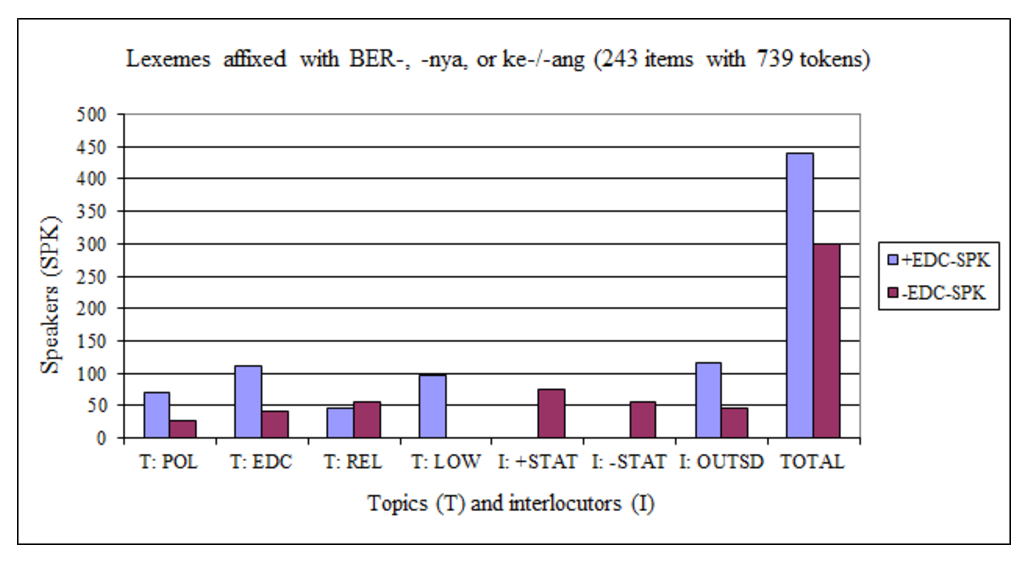
\includegraphics[scale=0.7]{./figures/Figure_3_4}
\resizebox{\textwidth}{!}{
\begin{tikzpicture}
  \begin{axis}[klugeaxis, y={}, height={.5\textheight}, width={\textwidth}, title={Lexemes affixed with \textscItal{ber}-, \textitbf{-nya}, or \textitbf{ke}\textitbf{-}/\textitbf{-}\textitbf{ang} (243 items with 739 tokens)}]
  \addplot[klugedots]	coordinates {(1,69)(2,112)(3,46)(4,97)(5,0)(6,0)(7,116)(8,440)};
  \addplot[klugelines] coordinates {(1,27)(2,40)(3,55)(4,0)(5,76)(6,55)(7,46)(8,299)};		
  \legend{\textsc{+edc-spk},\textsc{-edc-spk}}
  \end{axis}
  \end{tikzpicture}
  }
\caption[Token frequencies for lexemes affixed with {ber-}, \textitbf{-nya}, or \textitbf{ke}\textitbf{-}/\textitbf{-}\textitbf{ang} by speakers, topics, and interlocutors]{Token frequencies for lexemes affixed with \textscItal{ber-}, \textitbf{-nya}, or \textitbf{ke}\textitbf{-}/\textitbf{-}\textitbf{ang} by speakers, topics, and interlocutors}\label{Figure_3.4}
\end{figure}




The data presented in \tabref{Table_3.25} and \figref{Figure_3.4} shows that for the 243 affixed lexemes, most tokens (684/739 – 93\%) can be explained in terms of speaker education levels, topics, and/or role-relations between the speakers and their interlocutors (\textsc{ilct}).


Most tokens (440/739 – 60\%) were produced by \textsc{+edc-spk}, while 299/739 tokens (40\%) were produced by \textsc{-edc-spk}.

 
The \textsc{+edc-spk} produced about half of their tokens (227/440 – 52\%) when talking about \textsc{high} topics. Another 116/440 \textsc{+edc-spk} tokens (26\%) occurred during conversations with an outsider, namely the author (\textsc{outs}). The remaining 97/440 \textsc{+edc-spk} tokens (22\%) were produced during conversations with fellow-Papuans about \textsc{low} topics.



The \textsc{-edc-spk} produced 41\% of their tokens (122/299) while discussing \textsc{high} topics. Another 46/299 \textsc{-edc-spk} tokens (15\%) occurred during conversations with the author. The remaining \textsc{-edc-spk} tokens (131/299 – 44\%) were produced during conversations about \textsc{low} topics. Of these, 76/299 tokens (25\%) occurred when \textsc{-edc-spk} discussed \textsc{low} topics with \textsc{+stat} Papuans. The remaining 55/299 \mbox{\textsc{-edc-spk}} tokens (18\%) were produced during conversations with \textsc{-stat} Papuans, and 
therefore cannot be explained in terms of speaker education levels, topics, and/or role-relations. 
This total of 55 tokens refers to 7\% of the 739 tokens attested in the corpus.\footnote{As for the attested hapaxes, the findings of this domain analysis suggest that most are conditioned by the variables of speaker education levels, topics, and/or role-relations: 22/25 hapaxes prefixed with \textscItal{ber-}, 59/68 hapaxes suffixed with \textitbf{-nya}, and 18/22 hapaxes circumfixed with \textitbf{ke-}/\textitbf{-ang}. These items are best explained as code-switches with Indonesian. This leaves only three \textscItal{ber-}hapaxes, nine \textitbf{-nya}{}-hapaxes, and four \textitbf{ke-}/\textitbf{-ang}{}-hapaxes that are unaccounted for in terms of language external factors and that are likely to be the result of a productive \isi{word-formation} process. This, in turn, decreases the respective P values:
 
\begin{enumerate}[label=(\arabic*)]
\item for three \textscItal{ber-}hapaxes P=0.0183 (N=164) as opposed to P=0.0415 for 25 hapaxes (N=602) (N differs for the two P values, as six of the derived lexemes were excluded from the domain analysis),
\item for nine \textitbf{-nya}{}-hapaxes P=0.0284 (N=317) as opposed to P=0.1758 for 68 hapaxes (N=387) (N differs for the two P values, as one derived lexeme was excluded from the domain analysis), and
\item	 for four \textitbf{ke-}/\textitbf{-ang}{}-hapaxes P=0.0155 as opposed to P=0.0853 for 22 hapaxes (N=258).

\end{enumerate}
}

\section{Compounding}\label{Para_3.2}

Compounding denotes the “formation of a new lexeme by adjoining two or more lexemes” \citep[40]{Bauer.2003}. In Papuan Malay, however, the demarcation between compounds and phrasal expressions is unclear. That is, neither phonological, morphological, morphosyntactic, nor semantic criteria allow classifying word sequences unambiguously as either compounds or phrasal expressions, as shown in §\ref{Para_3.2.1}. The attested word combinations always have a binary structure in that they consist of two juxtaposed lexemes; the first component is always a \isi{noun}. More specifically, three types of word sequences can be distinguished, namely endocentric, exocentric, and coordinative ones, as discussed in §\ref{Para_3.2.2}. The main points on \isi{compounding} are summarized in §\ref{Para_3.3}.
 

\subsection{Demarcation of compounds from phrasal expressions}\label{Para_3.2.1}

Four different criteria have been suggested to distinguish compounds from phrasal expressions: phonological, morphological, morphosyntactic, and semantic criteria {\citep[24]{Aikhenvald.2007}}. They are discussed in turn in this section.



On phonological grounds, compounds can be distinguished from phrasal expressions in terms of their stress behavior. Compounds typically contain one primary stress, where\-as in phrasal expressions each phonological word carries its own stress {\citep[25]{Aikhenvald.2007}}. This criterion also applies to Papuan Malay, as shown in (\ref{Example_3.78}) and (\ref{Example_3.79}). In the \isi{compound} \textitbf{kacang-hijow} ‘mung bean’ in (\ref{Example_3.78}), the penultimate syllable carries primary stress, while secondary stress is assigned to the alternating syllable preceding the one carrying the primary stress. By contrast, in the \isi{phrasal expression} \textitbf{kacang hijow} ‘green bean’ in (\ref{Example_3.79}) each constituent carries its own stress. In fast speech, however, it is difficult to distinguish both constructions on phonological grounds. Instead, the context is the determining factor to establish the intended meaning.


% \todo{check example labelling}
\begin{styleExampleTitle}
{Phonological criteria}
\end{styleExampleTitle}
\ea
\label{Example_3.78}
\glll \textup{/ˌka.tʃaŋ.ˈhi.dʒɔw/} {} kacang-hijow\\ %
 { } { }  {bean-be.green}  \\
  { } { }  {‘mung bean’} \\
\z
\ea
\label{Example_3.79}
\glll \textup{/ˈka.tʃaŋ ˈhi.dʒɔw/} {}  kacang hijow\\ %
{} { }  {bean}  {be.green}  \\
{} { }  {‘green} {bean’} \\
\z


As for morphological criteria, compounds are typically distinct from phrasal expressions in that the former are marked with additional morphemes or have distinct constituent orders vis-à-vis phrasal expressions {\citep[26]{Aikhenvald.2007}}. In terms of morphological criteria, however, Papuan Malay compounds are not distinct from phrasal expressions. As illustrated in (\ref{Example_3.78}) and (\ref{Example_3.79}), neither construction has an additional morpheme that would mark it as a \isi{compound} or \isi{phrasal expression}. Neither are the two constructions distinct in terms of their constituent order, as in each case the head precedes the modifier.


On morphosyntactic grounds, compounds are usually distinct from phrasal expressions in that the components of a \isi{compound} cannot be separated by inserting other morphemes {\citep[26]{Aikhenvald.2007}}. Such an insertion leads to the loss of their \isi{compound} sense. This criterion also applies to Papuan Malay as shown in (\ref{Example_3.80}) and (\ref{Example_3.81}). When, for instance, the \isi{relativizer} \textitbf{yang} ‘\textsc{rel}’ is inserted in the \isi{compound} \textitbf{lemon-manis} ‘orange’ in (\ref{Example_3.80}), the \isi{compound} sense is lost. The result is the \isi{phrasal expression} \textitbf{lemon yang manis} ‘lemon which is sweet’ or ‘sweet lemon’ in (\ref{Example_3.81}).


 
\begin{styleExampleTitle}
{Morphosyntactic criteria}
\end{styleExampleTitle}
 
\ea
\label{Example_3.80}
\gll lemon-manis\\ %
lemon-be.sweet\\
 \glt ‘orange’\\
\z
 
\ea
\label{Example_3.81}
\gll lemon yang manis\\ %
{lemon} \textsc{rel} {be.sweet}\\
 \glt  ‘sweet lemon’ (Lit. ‘lemon which is sweet’)\\
\z



In cases such as the \isi{compound} \textitbf{orang-tua} ‘parent’ in (\ref{Example_3.82}) or the \isi{phrasal expression} \textitbf{orang tua} ‘old person’ in (\ref{Example_3.83}), however, it is difficult to distinguish both constructions on morphosyntactic grounds. Again, the context is the determining factor to establish the intended meaning.



\begin{styleExampleTitle}
{Ambiguities with respect to morphosyntactic criteria}
\end{styleExampleTitle} 
\ea
\label{Example_3.82}
\gll orang-tua\\ %
{person-be.old}\\
 \glt ‘parent’\\
\z 
\ea
\label{Example_3.83}
\gll orang tua\\ %
{person} {be.old}\\
 \glt ‘old person’\\
\z 


Semantically, compounds and phrasal expressions can be arranged on a scale from less to more compositional \citep[28]{Aikhenvald.2007}. The corpus, however, does not contain non-compositional compounds with idiosyncratic semantics.\footnote{While {\citet[28]{Aikhenvald.2007}} suggests that compounds can also be compositional, \citet[175]{Dryer.2007b} maintains that compounds have “an idiosyncratic meaning not predictable from the meaning of the component parts, as compared with syntactic compounds, in which one \isi{noun} is modifying a second \isi{noun} in a productive syntactic construction”.} This is illustrated in (\ref{Example_3.84}) to (\ref{Example_3.88}). Less compositional compounds are expressions such as \textitbf{kampung-tana} ‘home village’ in (\ref{Example_3.84}), or \textitbf{paduang-swara} ‘choir’ in (\ref{Example_3.85}). Compounds that are more compositional are those whose meaning is predictable from the meanings of its parts, such as \textitbf{air-mata} ‘tears’ in (\ref{Example_3.86}) or \textitbf{tali-prut} ‘intestines’ in (\ref{Example_3.87}). Very transparent compounds blend into phrasal expressions such as \textitbf{uang jajang} ‘pocket money’ or ‘money for snacks’ in (\ref{Example_3.88}). On the one hand one could say that \textitbf{uang jajang} ‘pocket money’ is a \isi{compound} with an idiosyncratic meaning. On the other hand one could argue that this construction has a phrasal structure that denotes a purpose relation between the nominal head \textitbf{uang} ‘money’ and its nominal modifier \textitbf{jajang} ‘snack’; hence, the construction \textitbf{uang jajang} ‘money for snacks’ is a \isi{phrasal expression} and not a \isi{compound}. Finally, there are phrasal expressions with clear compositional semantics, such as \textitbf{air sagu} ‘liquid of the sago palm tree’ in (\ref{Example_3.89}). (For details on \isi{noun} phrases with nominal modifiers see §\ref{Para_8.2.2}.)



\begin{styleExampleTitle}
{Semantic criteria}
\end{styleExampleTitle} 
\ea
\label{Example_3.84}
\gll kampung-tana\\ %
 village-ground\\
 \glt ‘home village’\\
\z  
\ea
\label{Example_3.85}
\gll paduang-swara\\ %
 fusion-voice\\
\glt 
‘choir’\\
\z 
\ea
\label{Example_3.86}
\gll air-mata\\ %
 water-eye\\ 
\glt  ‘tears’\\
\z 
\ea
\label{Example_3.87}
\gll tali-prut\\ %
 cord-stomach\\
\glt ‘intestines’\\
\z 
\ea
\label{Example_3.88}
\gll uang jajang\\ %
{money}  {snack}\\
\glt ‘pocket money’ / ‘money for snacks’\\
\z 
\ea
\label{Example_3.89}
\gll air  sagu\\ %
 {water} {sago} \\
\glt 
‘liquid of the sago palm tree’\\
\z

The data presented in this section shows that in Papuan Malay neither phonological, morphological, morphosyntactic, nor semantic criteria allow the unambiguous classification of word sequences as either compounds or phrasal expressions. Instead the data suggests that, following \citegen[14]{Lieber.2009} definition of \isi{compounding}, some Papuan Malay word combinations are “more compoundlike” while others are “less compoundlike [\ldots] with no clear categorical distinction” along this “cline”. The combinations range from less compositional two-word expressions such as \textitbf{kampung-tana} ‘home village’ to those with compositional transparent semantics such as \textitbf{air sagu} ‘liquid of the sago palm tree’. Given this lack of a clear demarcation between compounds and phrasal expressions, the term “\isi{collocation}” rather than “\isi{compound}” is used hereafter for such juxtaposed word sequences.\footnote{Collocations are defined as “word combinations which have developed an idiomatic semantic relation based on their frequent co-occurrence” (\citealt[200]{Bussmann.1996}; see also \citealt{Krishnamurthy.2006}).}


\subsection{Types of collocations}\label{Para_3.2.2}

In Papuan Malay, three types of collocations are found: endocentric, exocentric, and coordinative ones. In the following they are discussed one by one. 



In endocentric collocations, one component has head function while the subordinate component has modifying, content-specifying function, denoting “a sub-class of the items denoted by one of their elements” {\citep[42]{Bauer.2003}}. In Papuan Malay endocentric collocations, the head component always precedes the modifier component which can be a \isi{noun} or a stative \isi{verb}. Semantically, these ``\textsc{n} \textsc{n}'' or ``\textsc{n} \textsc{v}'' collocations encode different types of relationships between their components such as ``part-whole'', ``subtype-of'', or ``characteristic-of'' relations, as illustrated in \tabref{Table_3.26}. In addition, the corpus contains one \isi{collocation} in which the modifying component is a \isi{numeral}: \textitbf{segi-empat} ‘quadrangle’ (literally ‘side-four’).

\begin{table}
\caption{Endocentric ``\textsc{n} \textsc{n/v}'' collocations}\label{Table_3.26}

\begin{tabular}{llll}
\lsptoprule
 \multicolumn{1}{c}{Item} & \multicolumn{1}{c}{Gloss} & \multicolumn{1}{c}{Literal translation} &  \multicolumn{1}{c}{Semantic relation}\\
\midrule


\textitbf{tali-prut} & ‘intestines’ & ‘cord of the stomach’ & ‘Part-whole’\\

cord-stomach &  &  & \\
\\
\textitbf{lemon-manis} & ‘orange’ & ‘sweet lemon’ & ‘Subtype-of’\\

lemon-be.sweet &  &  & \\
\\
\textitbf{kreta-api} & ‘train’ & ‘carriage of fire’ & ‘Characteristic-of’\\

carriage-fire &  &  & \\

\lspbottomrule
\end{tabular}
\end{table}
% \todo[inline]{it is unclear to me how this should be modified}

In exocentric collocations, none of the constituents functions as its head. They “denote something which is not a sub-class” of either of their components; that is, “they are not hyponyms of either of their elements” {\citep[42]{Bauer.2003}}, as shown in \tabref{Table_3.27}. In the \isi{collocation} \textitbf{bapa-ade}, literally ‘father-younger.sibling’, for instance, neither of the two components serves as the content-specifying element. Likewise \textitbf{kepala-batu}, literally ‘head-stone’ does not refer to some kind of head. Instead, it denotes a ‘pig-headed person’. These examples also show that exocentric collocations typically consist of two juxtaposed nouns.

\begin{table}
\caption{Exocentric ``\textsc{n} \textsc{n}'' collocations}\label{Table_3.27}
\begin{tabular}{ll}
\lsptoprule
 \multicolumn{1}{c}{Item} & \multicolumn{1}{c}{Gloss}\\
\midrule

\textitbf{bapa-ade} & ‘father’s younger brother’(FyB) / ‘mother’s\\
father-ySb & younger sister’s husband’ (MyZH)\\
\tablevspace

\textitbf{kepala-batu} & ‘pig-headed person’\\
head-stone & \\
\tablevspace

\textitbf{mata-hari} & ‘sun’\\
eye-day & \\

\lspbottomrule
\end{tabular}
\end{table}


The distinction between endocentric and exocentric collocations is not always clear-cut, however, as shown in \tabref{Table_3.28}. The kinship terms \textitbf{bapa-tua} ‘uncle’ (literally ‘father-be.old’) and \textitbf{mama-tua} ‘aunt’ (literally ‘mother-be.old’) qualify as exocentric collocations on semantic grounds but as endocentric collocations on syntactic grounds. Both terms are exocentric in that they designate something which is not a sub-class of either of their components: \textitbf{bapa-tua} does not refer to an ‘old father’, neither does \textitbf{mama-tua} refer to an ‘old mother’. Instead, \textitbf{bapa-tua} denotes a ‘parent’s older brother’ (PoB) or a ‘parent’s older sister’s husband’ (PoZH), while \textitbf{mama-tua} designates a ‘parent’s older sister’ (PoZ) or a ‘parent’s older brother’s wife’ (PoBW). Syntactically, however, \textitbf{tua} ‘be old’ is subordinate to the head \textitbf{bapa}/\textitbf{mama} ‘father/mother’ and has modifying content-specifying function. Hence, both kinship terms also qualify as endocentric collocations.

\begin{table}
\caption{Endocentric versus exocentric collocations: Ambiguities}\label{Table_3.28}


\begin{tabular}{ll}
\lsptoprule
 \multicolumn{1}{c}{Item} &  \multicolumn{1}{c}{Gloss}\\
\midrule
\textitbf{bapa-tua} & ‘parent’s older brother’ (PeB) / ‘mother’s\\
father-be.old & ‘parent’s older sister’s husband’ (PeZH)\\
\tablevspace
\textitbf{mama-tua} & ‘parent’s older sister’ (PeZ) / ‘mother’s\\
mother-be.old & ‘parent’s older brother’s wife’ (PeBW)\\
\lspbottomrule
\end{tabular}
\end{table}

 

\begin{table}
\caption{Coordinative ‘\textsc{n} \textsc{n}’ collocations}\label{Table_3.29}


\begin{tabular}{lll}
\lsptoprule
 \multicolumn{1}{c}{Item} & \multicolumn{1}{c}{Gloss} &  \multicolumn{1}{c}{Semantic relation}\\
\midrule

\textitbf{ade-kaka} & siblings & Antonyms\\

ySb-oSb &  & \\
\\
\textitbf{kasi-sayang} & ‘deep love’ & Synonyms\\

love-love &  & \\
\\
\textitbf{guntur-kilat} & ‘thunderstorm’ & Different parts/aspects\\

thunder-lightning &  & \\
\\
\textitbf{tete-moyang} & ‘ancestors’ & Different parts/aspects\\

grandfather-ancestor &  & \\

\lspbottomrule
\end{tabular}
\end{table}

 Coordinative collocations designate entities made up of two nominal components that “can be interpreted as being joined by ‘and’” {\citep[351]{Bauer.2009}}. That is, in such collocations both components “are of semantically equal weight” {\citep[221]{Bussmann.1996}}. The nominal components can be antonyms, synonyms, or different parts or aspects of the designated concept, as shown in \tabref{Table_3.29}.

 
 \newpage 
\section{Summary}\label{Para_3.3}
\largerpage
This section briefly summarizes the main points on \isi{affixation} and \isi{compounding}.


\begin{enumerate}
\item 
Affixation


Affixation in Papuan Malay has very limited productivity. This conclusion is based on an investigation of six affixes: the prefixes \textscItal{ter-} ‘\textsc{acl}’, \textscItal{pe(n)-} ‘\textsc{ag}’, and \textscItal{ber-} ‘\textsc{vblz}’, the suffixes -\textitbf{ang} ‘\textsc{pat}’ and \textitbf{-nya} ‘\textsc{3possr}’, and the circumfix \textitbf{ke}-/-\textitbf{ang} ‘\textsc{nmlz}’. Given the \isi{sociolinguistic profile} of Papuan Malay (substantial language contact between Papuan Malay and Indonesian with both languages being in a diglossic distribution, positive to somewhat am\isi{bivalent} language attitudes toward Papuan Malay, and lack of language awareness of many Papuan Malay speakers) no productivity testing was conducted, as a substantial amount of interference from Indonesian was expected. This interference would have skewed testees’ naïve judgments. Instead, the six affixes were examined in terms of six language internal and three language external factors considered relevant in establishing the degree of productivity of these affixes.



The results of this investigation are as follows:
\begin{enumerate}

\item 
Papuan Malay \textscItal{ter-} ‘\textsc{acl}’ has limited productivity; it indicates accidental or unintentional actions or events. In other \ili{eastern Malay varieties} and in Standard Malay, the prefix is rather productive; here it likewise signals accidental or unintentional actions or events.
\item 
Papuan Malay -\textitbf{ang} ‘\textsc{pat}’ has limited productivity; it typically designates the patient or result of an action, event or state. As for other \ili{eastern Malay varieties}, the suffix is only mentioned for \ili{Ambon Malay}; its degree of productivity is unclear. In Standard Malay the suffix is very productive. Both in Ambon and in Standard Malay, the suffix also indicates the patient or product of an action, event or state.
\item 
Papuan Malay \textscItal{pe(n)-} ‘\textsc{ag}’ has marginal productivity, at best. It typically denotes the subject of the action, event, or state specified by the \isi{verbal base}; some of the affixed lexemes also receive an intensified intransitive or monotransitive reading. As for other \ili{eastern Malay varieties}, the prefix seems to have retained its productivity only in \ili{Ternate Malay}. In Standard Malay, the suffix is very productive. In other Malay varieties the prefix likewise denotes the subject of the action, event, or state specified by the \isi{verbal base}. A verbal interpretation, but not the intensified reading, is also reported for other \ili{eastern Malay varieties}. In Standard Malay, by contrast, only derivations with \isi{monovalent} stative bases can function as \isi{monovalent} stative verbs.
\item 
In Papuan Malay, prefix \textscItal{ber-} ‘\textsc{vblz}’ is unproductive, whereas in other \ili{eastern Malay varieties} and Standard Malay the prefix is very productive.
\item 
In Papuan Malay, \textitbf{-nya} ‘\textsc{3possr}’ and \textitbf{ke}\textitbf{-}/\textitbf{-}\textitbf{ang} ‘\textsc{nmlz}’ are unproductive. The same applies to other \ili{eastern Malay varieties}, while both affixes are very productive in Standard Malay.
\end{enumerate}

\item 
Compounding


In Papuan Malay, the demarcation between compounds and phrasal expressions is unclear. Neither phonological, morphological, morphosyntactic, nor semantic criteria allow the unambiguous classification of two juxtaposed nouns as compounds or phrasal expressions. Therefore, the term “\isi{collocation}” is employed as a cover term for such word combinations that differ in transparency from non-com\-posi\-tional idiosyncratic semantics to compositional transparent semantics. Three different types of collocations are attested, endocentric, exocentric, and coordinative ones. Given the lack of a clear demarcation between compounds and phrasal expressions, it remains unclear to what degree \isi{compounding} is a productive process.
\end{enumerate}
